\documentclass[12pt,letterpaper]{article}
\usepackage[utf8]{inputenc}
\usepackage{geometry}
\geometry{margin=1in}
\usepackage{setspace}
\usepackage{graphicx}
\usepackage{booktabs}
\usepackage{hyperref}
\hypersetup{
  pdftitle={Cultural Matching and the Persistence of Social Ties},
  pdfauthor={Omar Lizardo},
  colorlinks=true,
  linkcolor={blue},
  filecolor={maroon},
  citecolor={blue},
  urlcolor={blue}
}
\usepackage{titlesec}
\usepackage[round]{natbib}

\title{Folk Models of Good and Bad Taste: \\ A Computational Text Analysis}
\author{Omar Lizardo \\ Department of Sociology, UCLA}
\date{\today}

\begin{document}

\maketitle

\begin{abstract}
\noindent Sociologists have long debated the nature of ``good'' and ``bad'' taste, yet how lay individuals actually define these categories remains under-explored. Using open-ended survey responses, this research note applies BERTopic to inductively map folk cultural models of taste definitions and examples. I identify distinct cultural models for ``good taste'' (e.g., Subjectivity, Aesthetics, Fashion) and ``bad taste'' (e.g., Dislike, Poor Choices, Vulgarity). Chi-square cross-tabulations reveal that these cultural models form internally coherent cultural logics across both positive and negative evaluations. Furthermore, heatmaps mapping these cultural models onto 19 specific cultural domains reveal that while core domains like Music and Clothing are universally subjected to taste distinctions, moralized cultural models (e.g., citing Donald Trump or the Obamas) are associated with a heightened propensity to draw taste boundaries across nearly all domains.
\end{abstract}

% \doublespacing
\newpage
\section{Introduction}

The sociological study of cultural stratification has traditionally focused on how cultural consumption patterns map onto social hierarchies \citep{bourdieu1984distinction-835}. However, theoretical conceptualizations of ``good'' and ``bad'' taste are rarely compared against how everyday people implicitly define these constructs, although some recent interview-based work has begun to plumb this subject \citep{haak2019struggling-502, jarness2017im-001}. Do people view good taste as an aesthetic achievement, a moral disposition, or mere consensus with dominant trends? Better understanding these folk models of taste can provide vital insight into the contemporary boundaries of cultural inclusion and exclusion.

\section{Research Questions}

This research note is guided by three primary research questions:
\begin{enumerate}
    \item What are the distinct, latent cultural models that lay individuals use to define and provide examples of ``good taste'' and ``bad taste''?
    \item How do cultural models of good taste relate to cultural models of bad taste? Are they structurally coupled into broader cultural logics?
    \item How do these taste cultural models map onto specific cultural domains (e.g., beer, classical music, wrestling)? 
\end{enumerate}

\section{Methods}

Data for this study are drawn from an open-access dataset originally collected by Bonard, Cova, and Humbert-Droz (2024). In this study, researchers collected data from a representative sample of the US adult population ($N=297$) through the \textit{Prolific} Academic platform. After screening for data quality using four attention checks, the final sample comprised 241 participants (124 men, 114 women, 3 other; $M_{age} = 44.92$, $SD_{age} = 16.12$). In their survey, respondents were asked whether they distinguish between good and bad taste in their daily lives. The overwhelming majority of the sample (93\%, $N=224$) answered affirmatively. This subset was then asked to provide brief, open-ended definitions and concrete examples of both concepts.

To analyze these short, unstructured participant-level text responses (hereafter ``documents''), I used \textbf{BERTopic}. During preprocessing, domain-specific survey artifacts (e.g., ``good,'' ``bad,'' ``taste,'' ``don't'') were removed from each document because these words---mostly paraphrasing the original question---were overwhelmingly common across documents and thus did little to differentiate them. We also remove common English stop words from each document (e.g., the, it, is, do, etc.). The algorithm was optimized for each of the four text fields independently to prevent vocabulary blurring. Finally, cross-tabulations and domain-distinction Likert scale heatmaps were generated to examine the coherence of these classifications.

\section{Results}

\subsection{Cultural Models of Taste}

The BERTopic models identified distinct cultural models for definitions and examples. For \textbf{Good Taste}, respondents defined the concept primarily through \emph{Similarity/Subjectivity} (homophily), \emph{Aesthetics}, or \emph{Style/Quality}. When asked for concrete examples, the clusters were much richer, featuring groups who cited \emph{Fashion/Decor} (friends and spouses), \emph{Refinement/Art} (creators like Steve Jobs), \emph{Musical Knowledge}, or even specific public figures representing class like \emph{The Obamas}.

\begin{table}[htpb]
\centering
\resizebox{\textwidth}{!}{
\begin{tabular}{llll}
\toprule
Topic & Count & Name & Keywords \\
\midrule
-1 & 32 & -1\_fashion\_trendy\_style\_appreciate & fashion, trendy, style, appreciate, clothes, opinion, music, say, art, prefer \\
0 & 113 & 0\_say\_mean\_usually\_subjective & say, mean, usually, subjective, food, quality, enjoy, sense, certain, similar \\
1 & 62 & 1\_art\_appreciate\_choices\_shows & art, appreciate, choices, shows, look, enjoy, understand, pleasing, appealing, gaudy \\
2 & 16 & 2\_interact\_services\_selection\_look & interact, services, selection, look, style, way, choices, goods, interests, dress \\
\bottomrule
\end{tabular}
}
\caption{Good Taste Summary Table}
\label{tab:good_taste_summary_table}
\end{table}

\begin{table}[htpb]
\centering
\resizebox{\textwidth}{!}{
\begin{tabular}{lllll}
\toprule
Topic & Count & Name & Keywords & Example\_Responses \\
\midrule
-1 & 32 & -1\_fashion\_trendy\_style\_appreciate & fashion, trendy, style, appreciate, clothes, opinion, music, say, art, prefer & Outliers \\
0 & 113 & 0\_say\_mean\_usually\_subjective & say, mean, usually, subjective, food, quality, enjoy, sense, certain, similar & • "I think that a person who has good taste can easily influence a lot of people. I also think that they are very smart in knowing what their audience want. They follow modern trends and study the good and bad."• "Usually, when someone has good taste I consider their likes/dislikes to be similar to mine, because I believe that I have good taste." \\
1 & 62 & 1\_art\_appreciate\_choices\_shows & art, appreciate, choices, shows, look, enjoy, understand, pleasing, appealing, gaudy & • "This person can distinguish good art from bad art. This person has seen and learned a lot in this professional area."• "As elitist as it may sound, I've associated someone having good taste as someone rather cultured. Their preferences are somewhat subdued, and with a sense of cohesiveness. It's not loud, garish, or pretentious." \\
2 & 16 & 2\_interact\_services\_selection\_look & interact, services, selection, look, style, way, choices, goods, interests, dress & • "I think that they make good, stylish choices based on the type of aesthetic that I myself appreciate. They also think in creative ways that complement their choices as a whole."• "The have knowledge and range in the music they prefer" \\
\bottomrule
\end{tabular}
}
\caption{Good Taste Examples Table}
\label{tab:good_taste_examples_table}
\end{table}


For \textbf{Bad Taste}, respondents defined it through \emph{Subjective Dislike}, \emph{Poor Choices/Lack of Effort}, \emph{Tackiness/Gaudiness}, \emph{Low-Brow Media}, or \emph{Poor Manners/Immorality}. Concrete examples similarly ranged from \emph{Poor Fashion}, \emph{Derivative Media} (e.g., formulaic filmmakers), to specific instances of \emph{Vulgarity} (often citing Donald Trump).

\begin{table}[htpb]
\centering
\resizebox{\textwidth}{!}{
\begin{tabular}{llll}
\toprule
Topic & Count & Name & Keywords \\
\midrule
-1 & 38 & -1\_quality\_poor\_dont\_art & quality, poor, dont, art, understanding, clothing, usually, value, negative, content \\
0 & 106 & 0\_say\_dont\_likes\_example & say, dont, likes, example, usually, does, different, mean, doesnt, opinion \\
1 & 61 & 1\_dont\_choices\_care\_make & dont, choices, care, make, maybe, poorly, gaudy, art, value, andor \\
2 & 18 & 2\_loud\_sense\_colors\_shows & loud, sense, colors, shows, qualities, character, boo, drama, bold, similar \\
\bottomrule
\end{tabular}
}
\caption{Bad Taste Summary Table}
\label{tab:bad_taste_summary_table}
\end{table}

\begin{table}[htpb]
\centering
\resizebox{\textwidth}{!}{
\begin{tabular}{lllll}
\toprule
Topic & Count & Name & Keywords & Example\_Responses \\
\midrule
-1 & 38 & -1\_quality\_poor\_dont\_art & quality, poor, dont, art, understanding, clothing, usually, value, negative, content & Outliers \\
0 & 106 & 0\_say\_dont\_likes\_example & say, dont, likes, example, usually, does, different, mean, doesnt, opinion & • "A person has bad taste when they don't follow current trends. They are unable to think outside the box and refuse to see things from different points of view. They get stuck in one thing and end up getting left behind."• "If majority of people think what they think is good is bad then it usually means they have bad taste compared to everyone." \\
1 & 61 & 1\_dont\_choices\_care\_make & dont, choices, care, make, maybe, poorly, gaudy, art, value, andor & • "Bad taste is noted when others do not approve of someone's choices or biases on a particular topic. It could mean that they are behind on following trends, or it could mean that they fail to see the depth or true value in the aforementioned topic and have shallow judgement."• "Someone who watches conspiracy theory shows and drama based reality TV about people’s personal lives. Ancient Aliens and similar shows acively try to mislead people. Shows like Honey Boo Boo and similar just encourage drama amongst the people involved." \\
2 & 18 & 2\_loud\_sense\_colors\_shows & loud, sense, colors, shows, qualities, character, boo, drama, bold, similar & • "I'd say someone with a "bad taste" doesn't really like things on their own, they tend to be a follower for what's popular so they don't end up with much of a taste at all. I'd also say it's when they like a lot of things that other people tend to dislike, so they'd have a "bad taste" compared. Again though, really depends on cultures and areas they grew up, what may be bad tastes where they are, could be good tastes elsewhere."• "Someone who behaves with vulgarity, or who likes cheap furniture or art." \\
\bottomrule
\end{tabular}
}
\caption{Bad Taste Examples Table}
\label{tab:bad_taste_examples_table}
\end{table}


\begin{figure}[htpb]
    \centering
    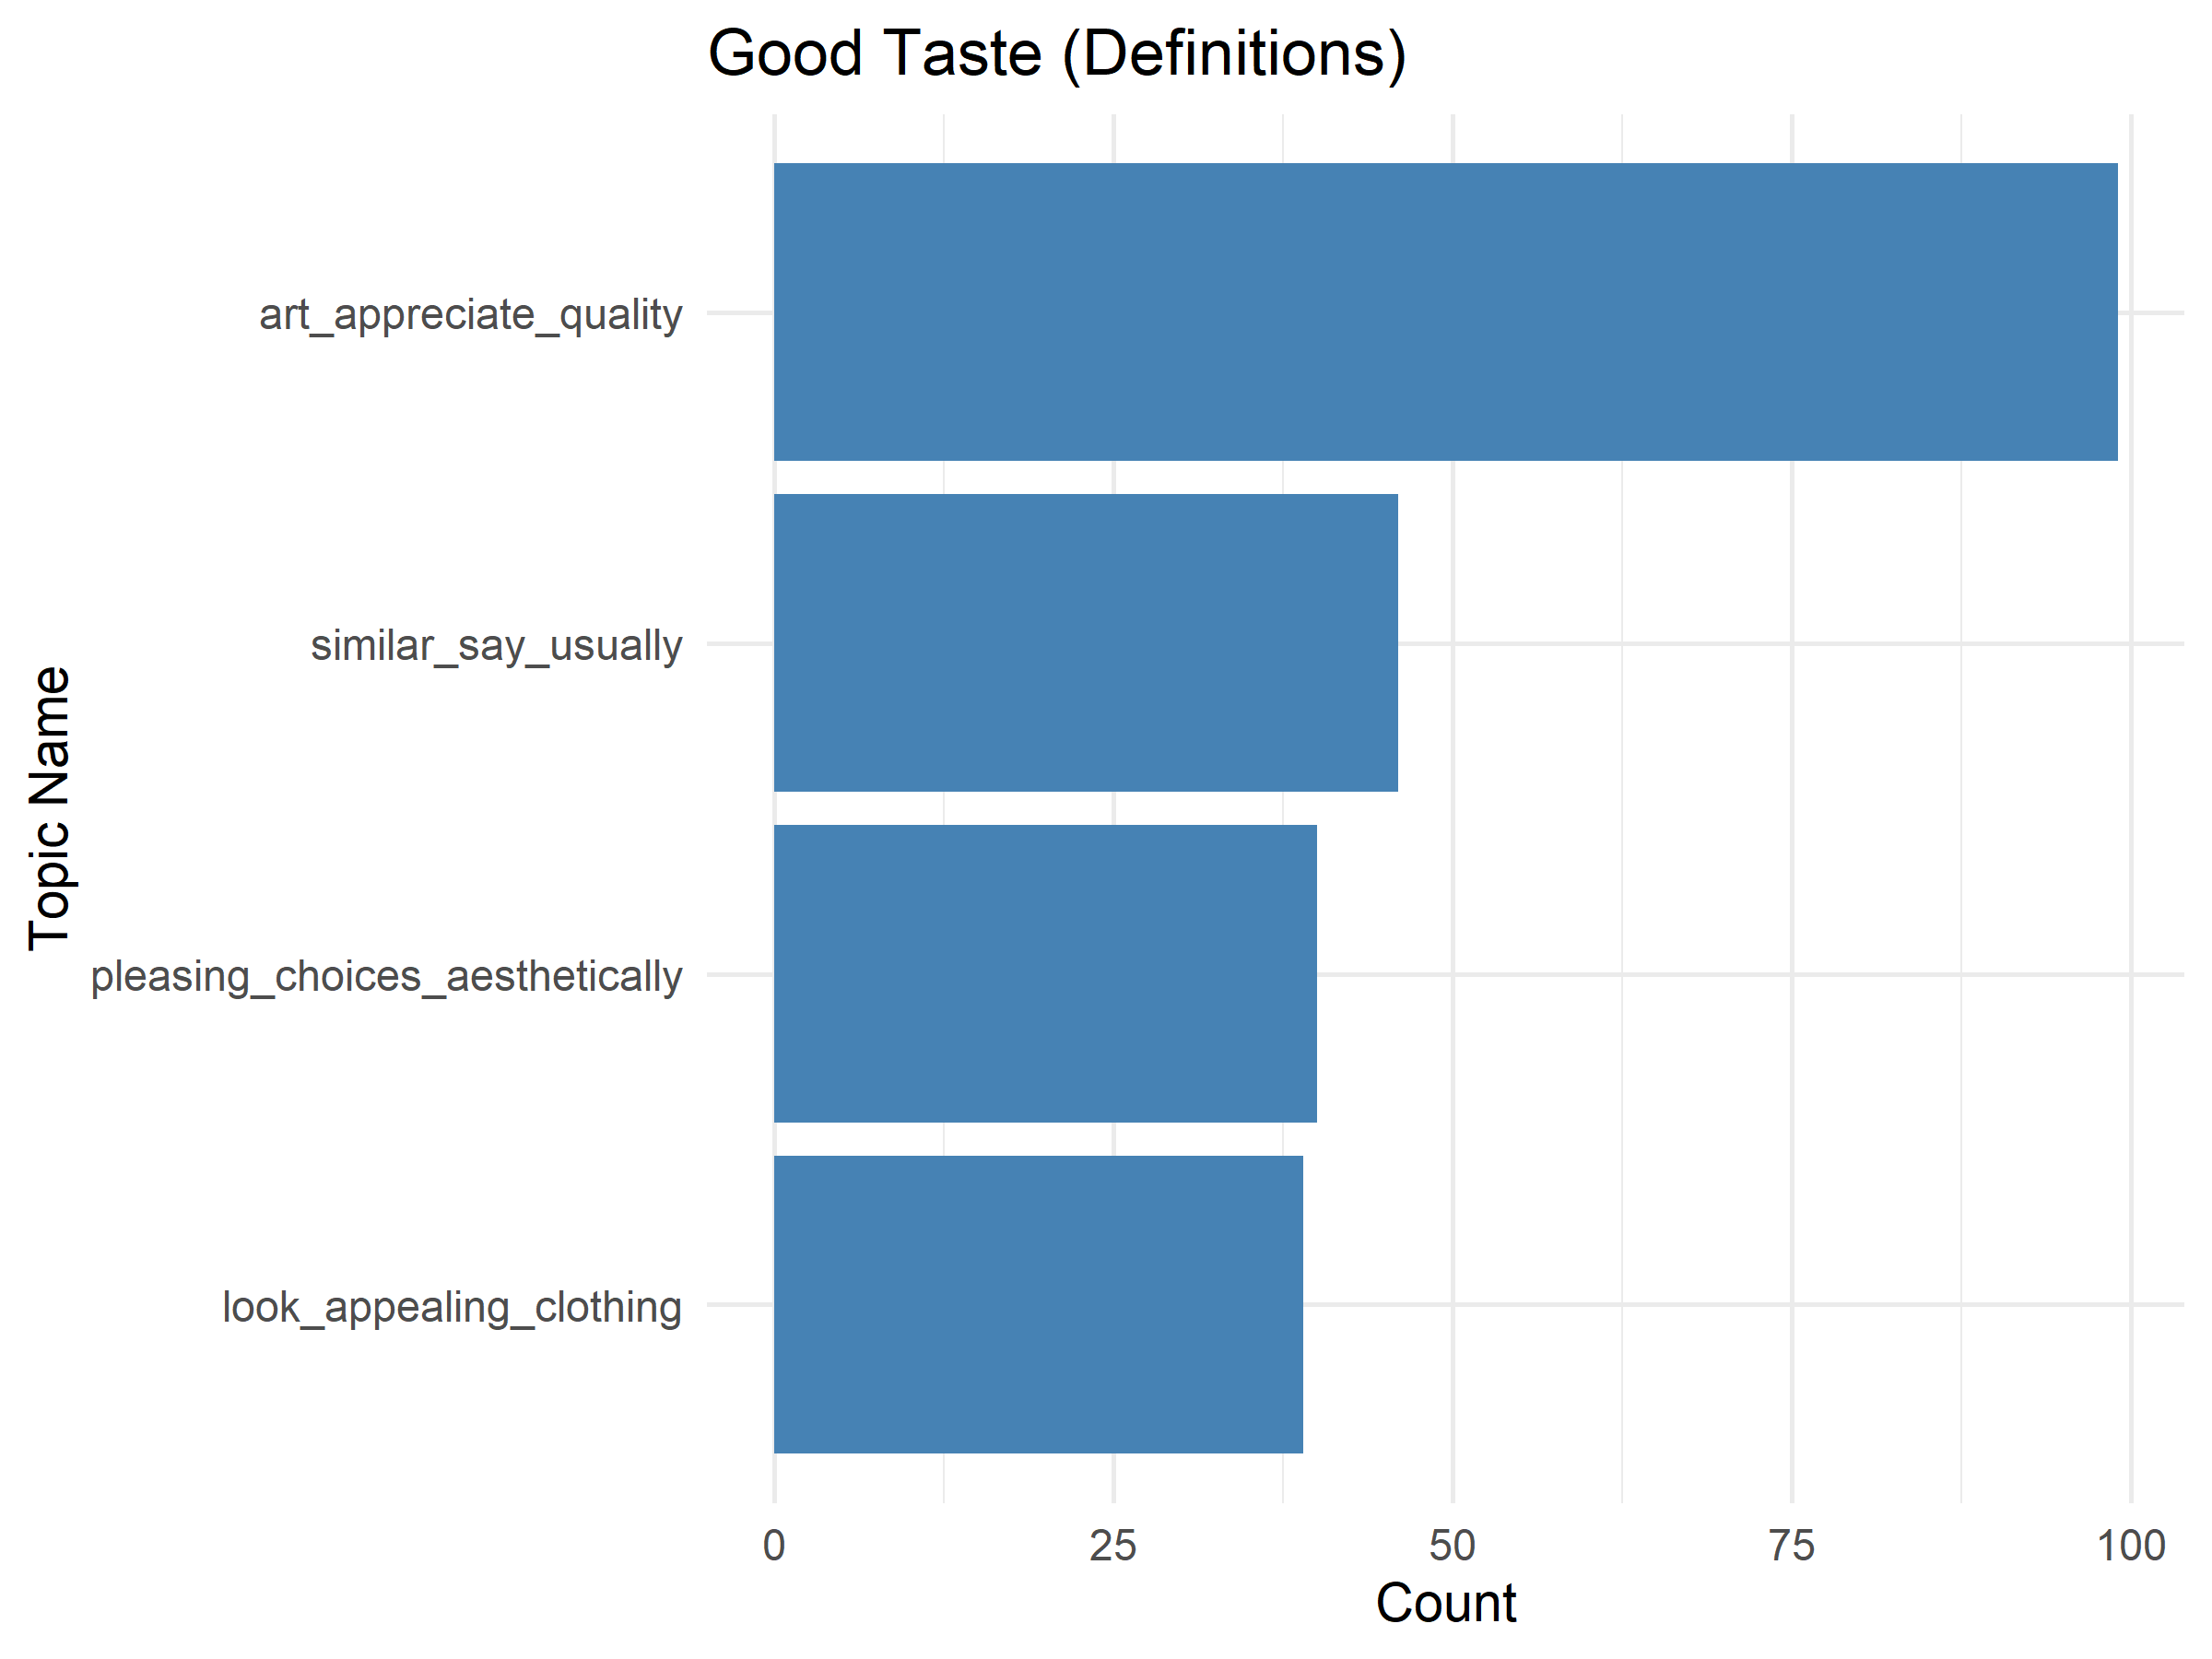
\includegraphics[width=0.48\textwidth]{report/Plots/good_taste_topics.png}
    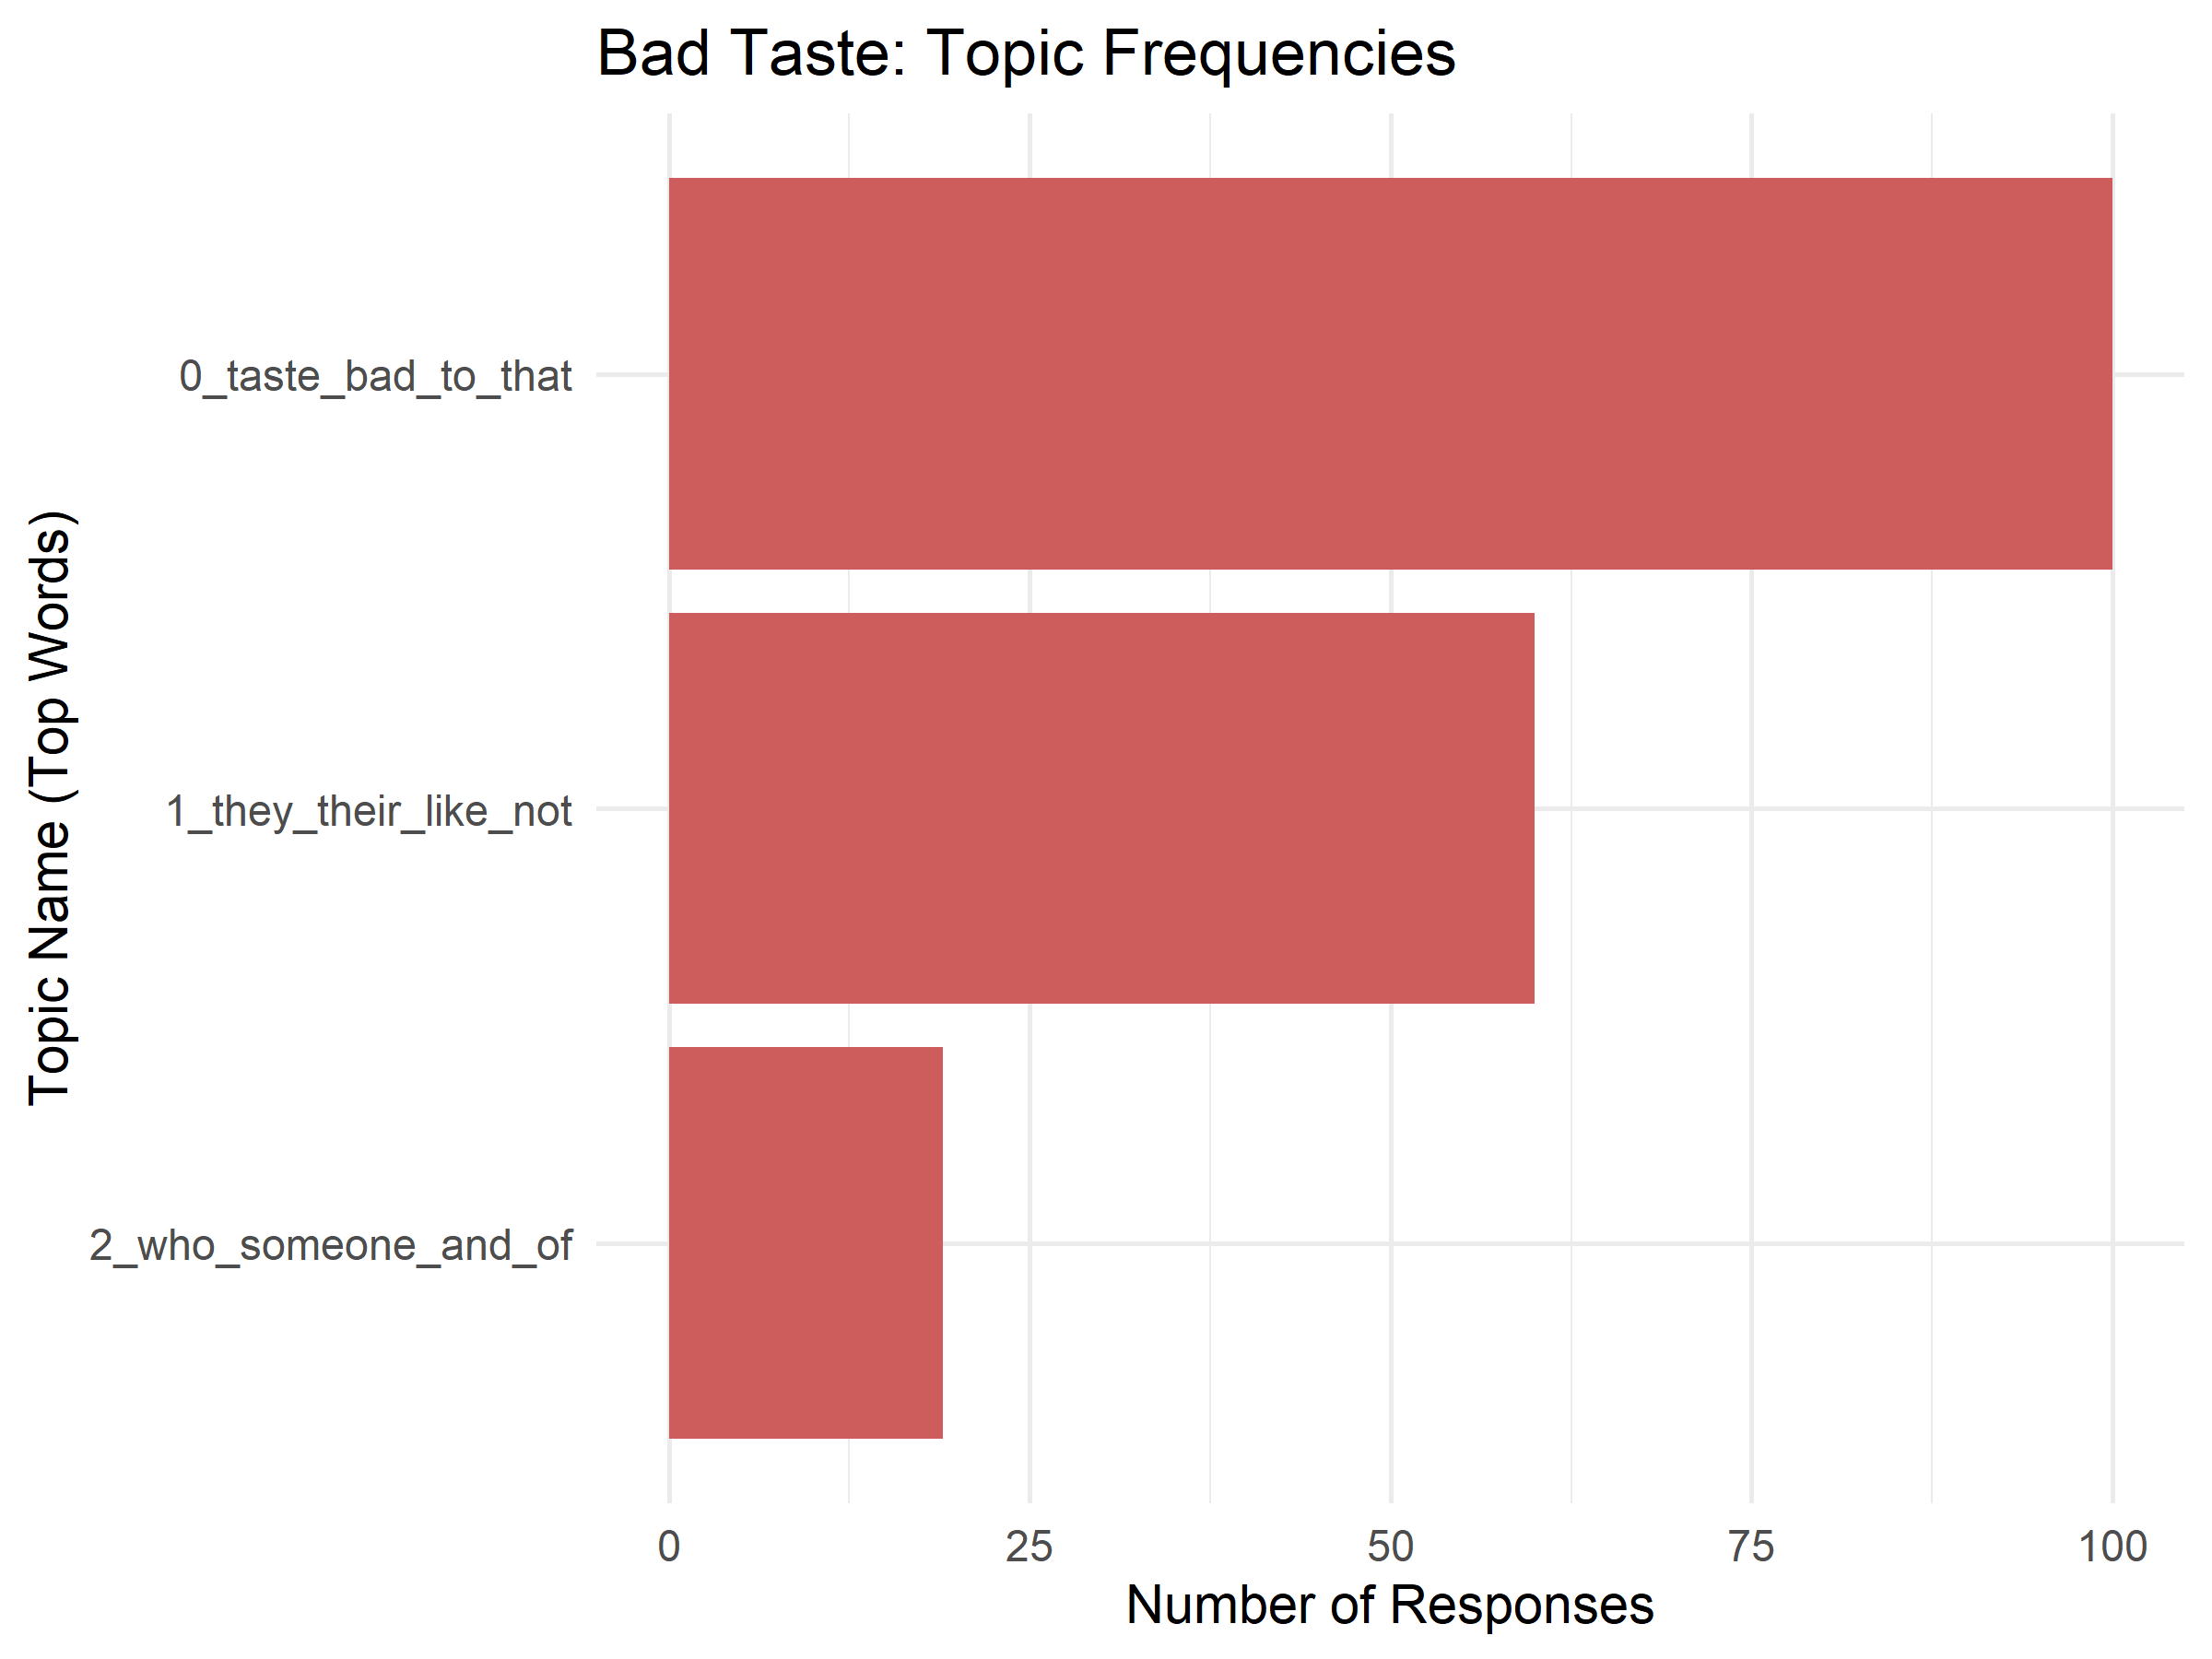
\includegraphics[width=0.48\textwidth]{report/Plots/bad_taste_topics.png}
    \caption{Topic Frequencies for Good and Bad Taste (Definitions)}
    \label{fig:topic_frequencies_def}
\end{figure}

\begin{figure}[htpb]
    \centering
    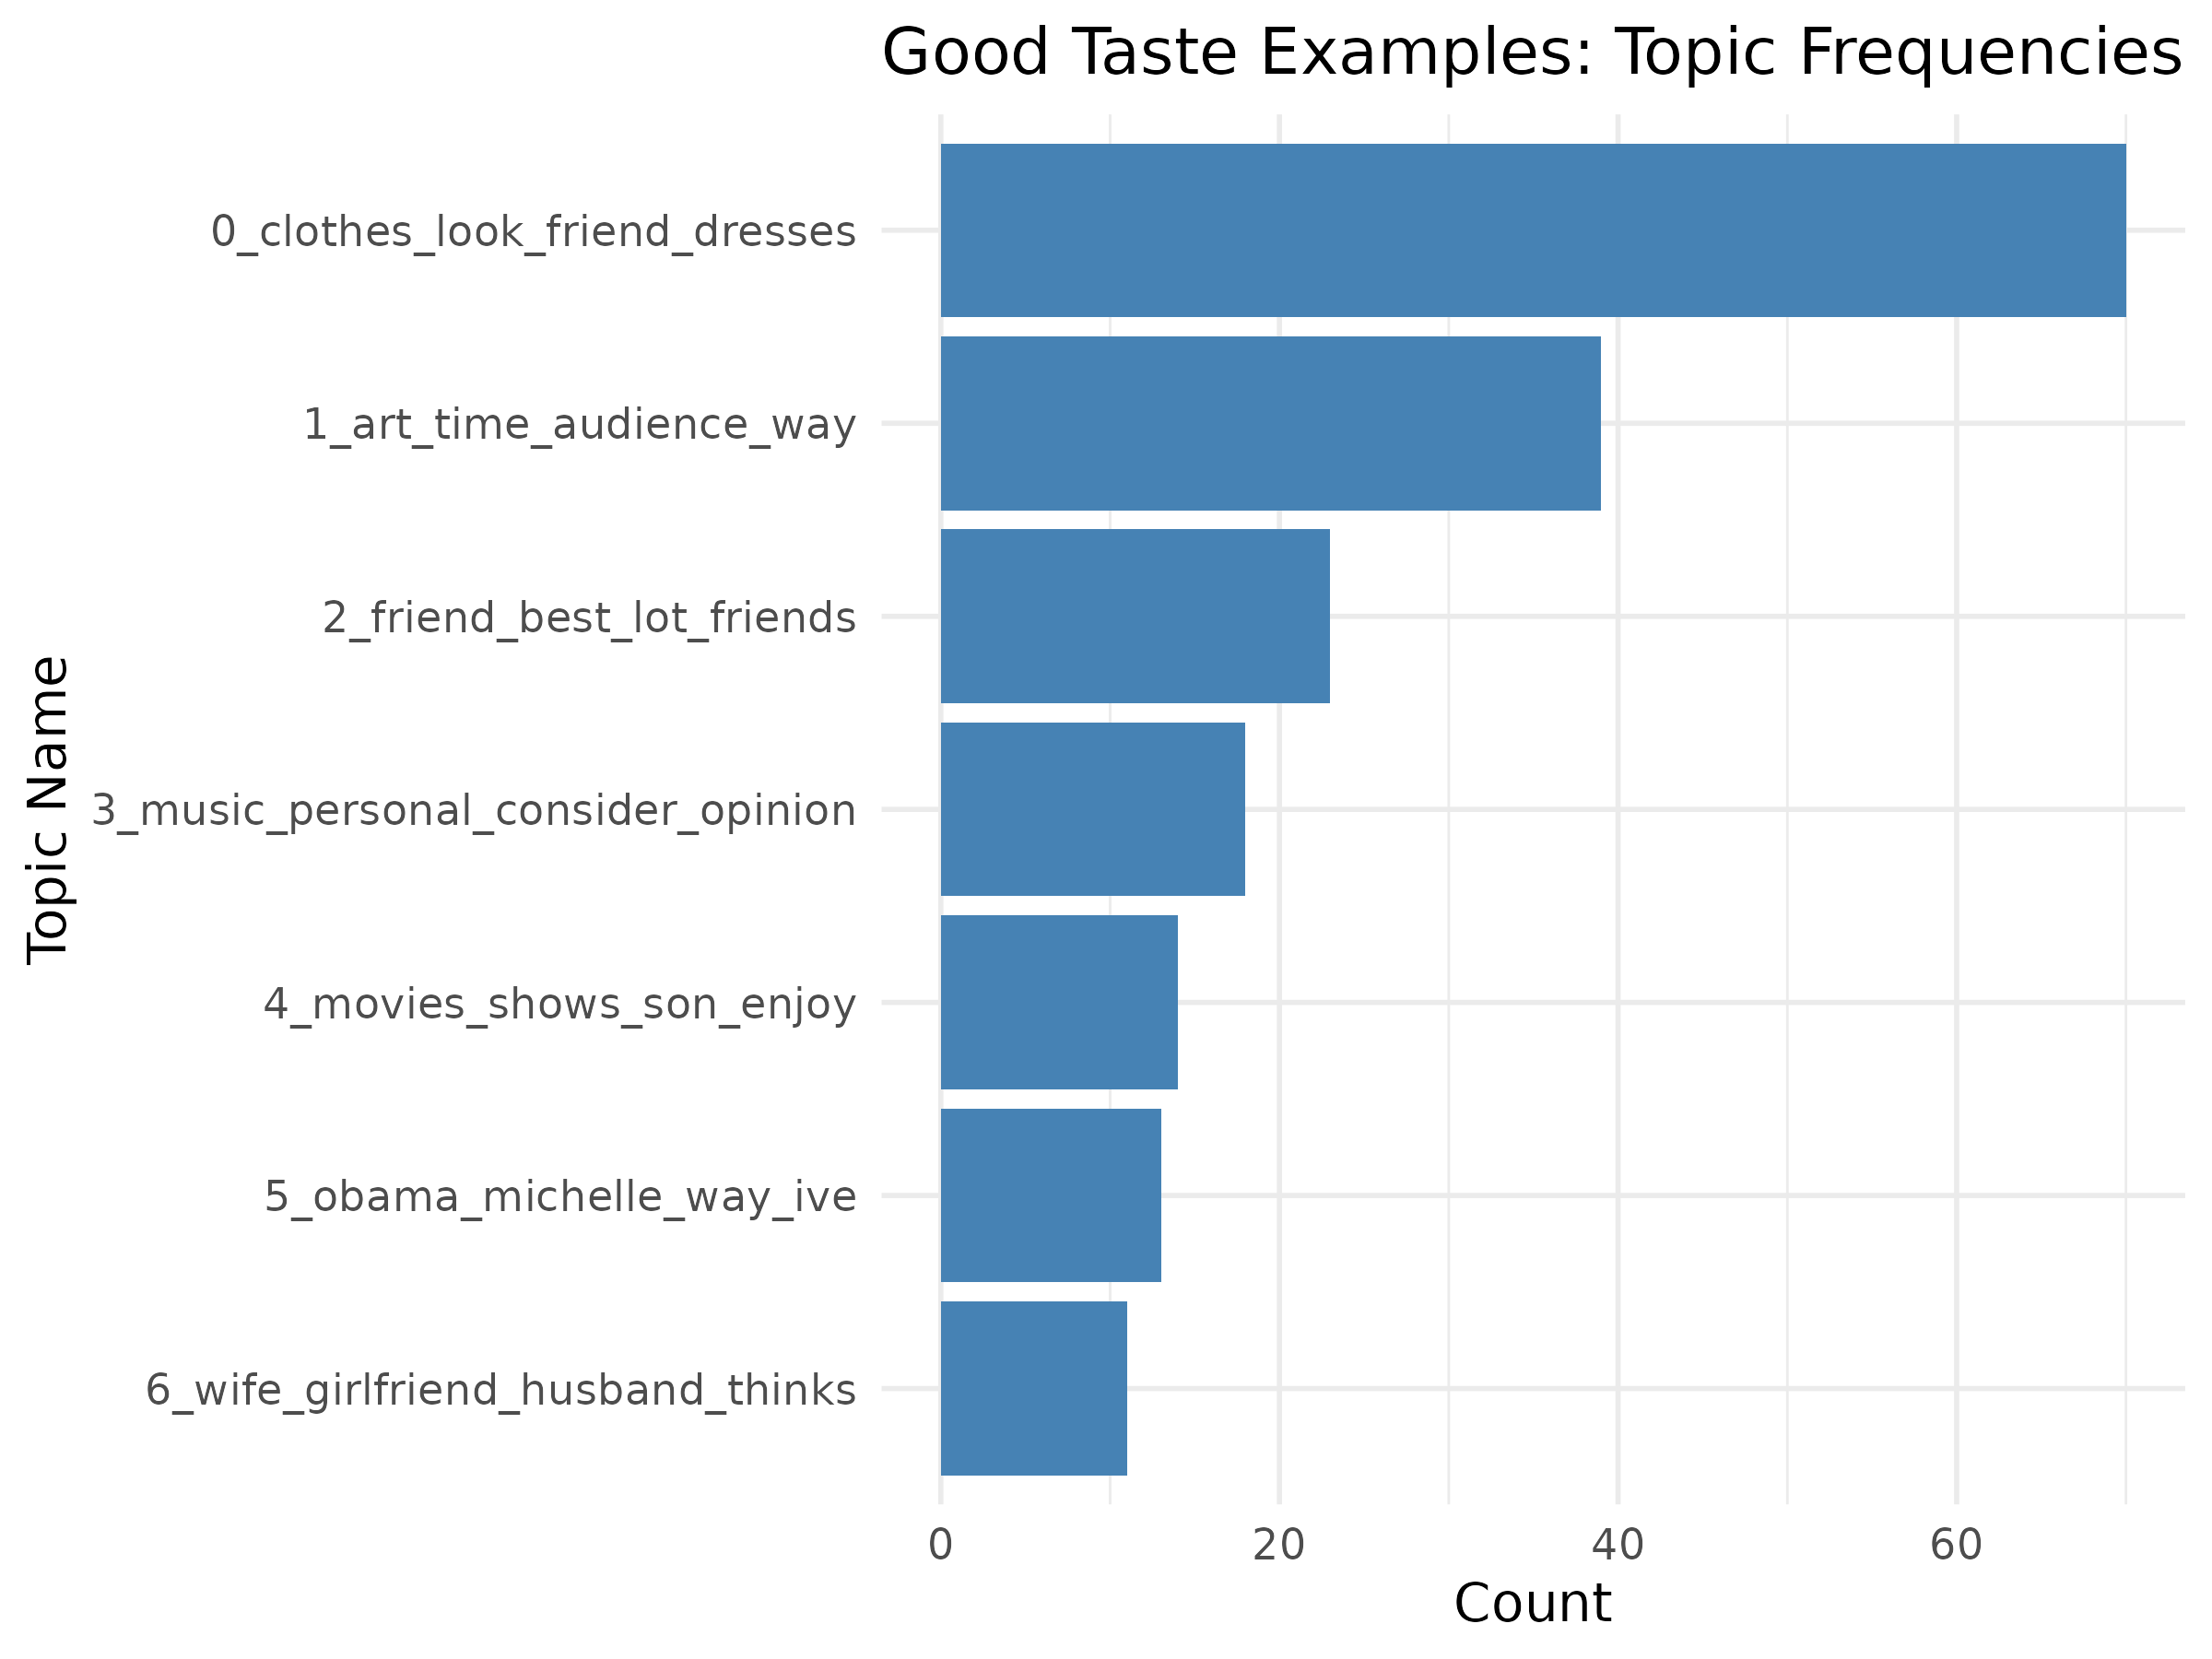
\includegraphics[width=0.48\textwidth]{report/Plots/good_taste_example_topics.png}
    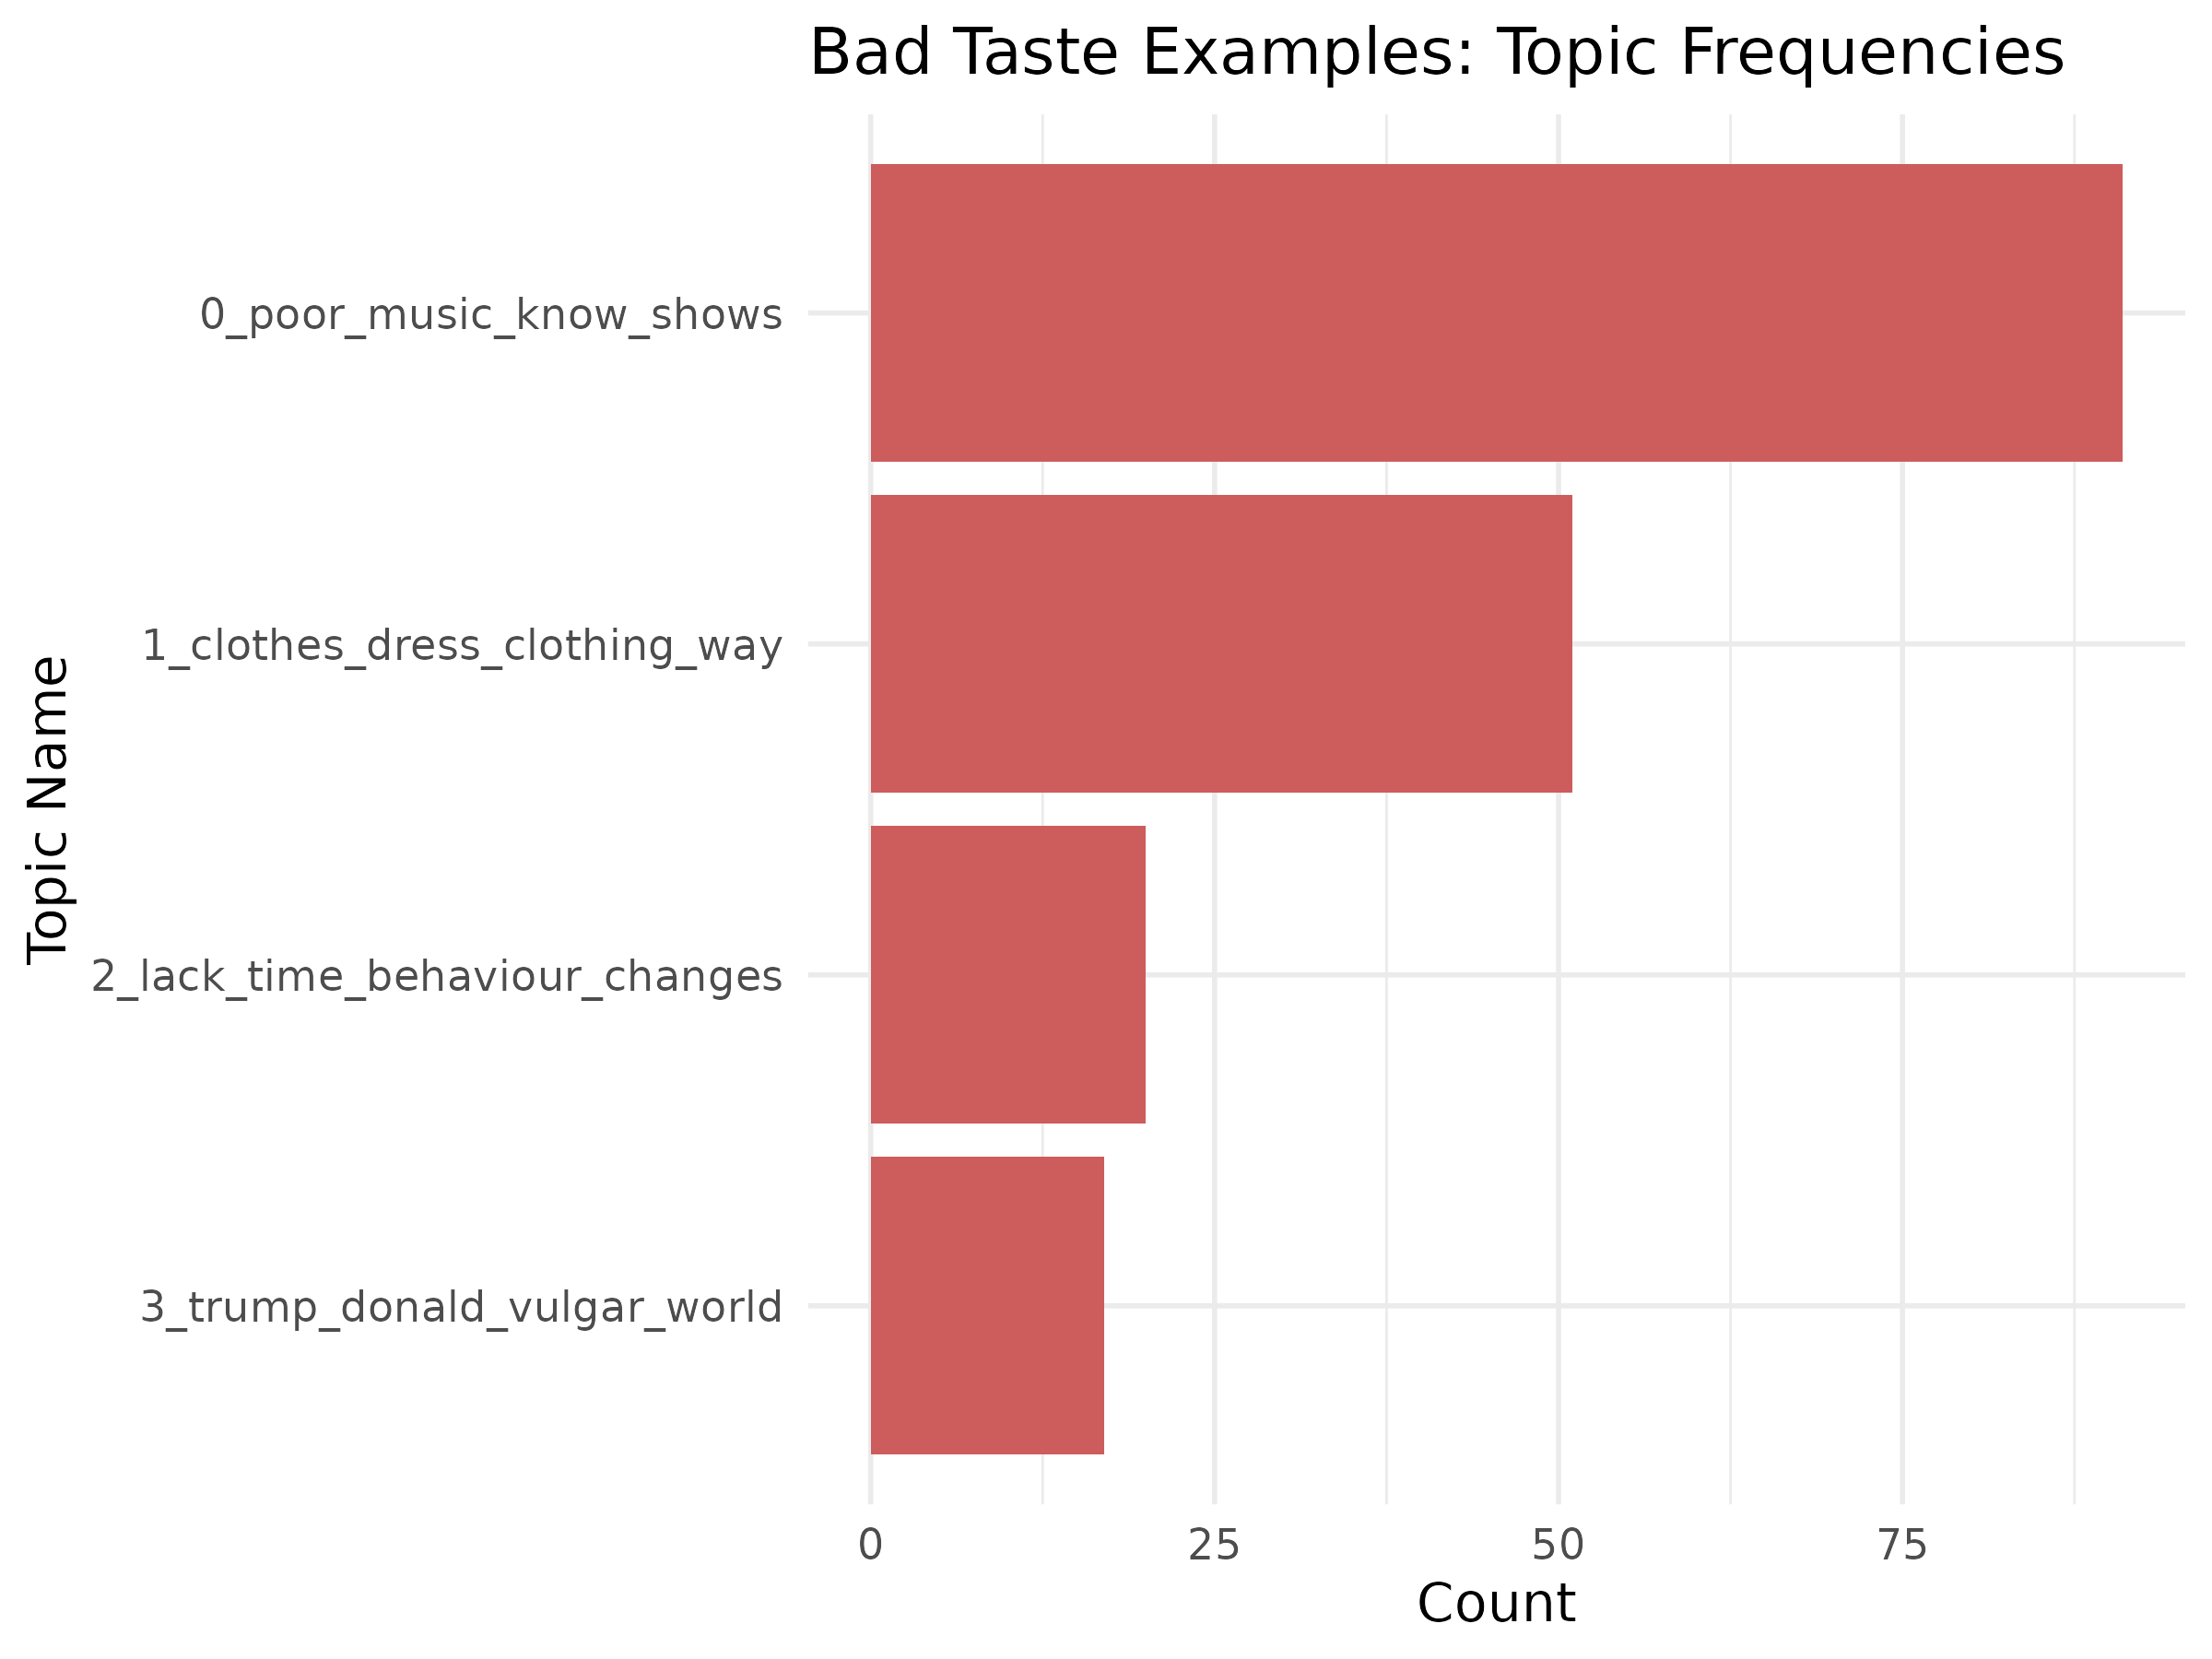
\includegraphics[width=0.48\textwidth]{report/Plots/bad_taste_example_topics.png}
    \caption{Topic Frequencies for Good and Bad Taste (Examples)}
    \label{fig:topic_frequencies_ex}
\end{figure}

\begin{figure}[htpb]
    \centering
    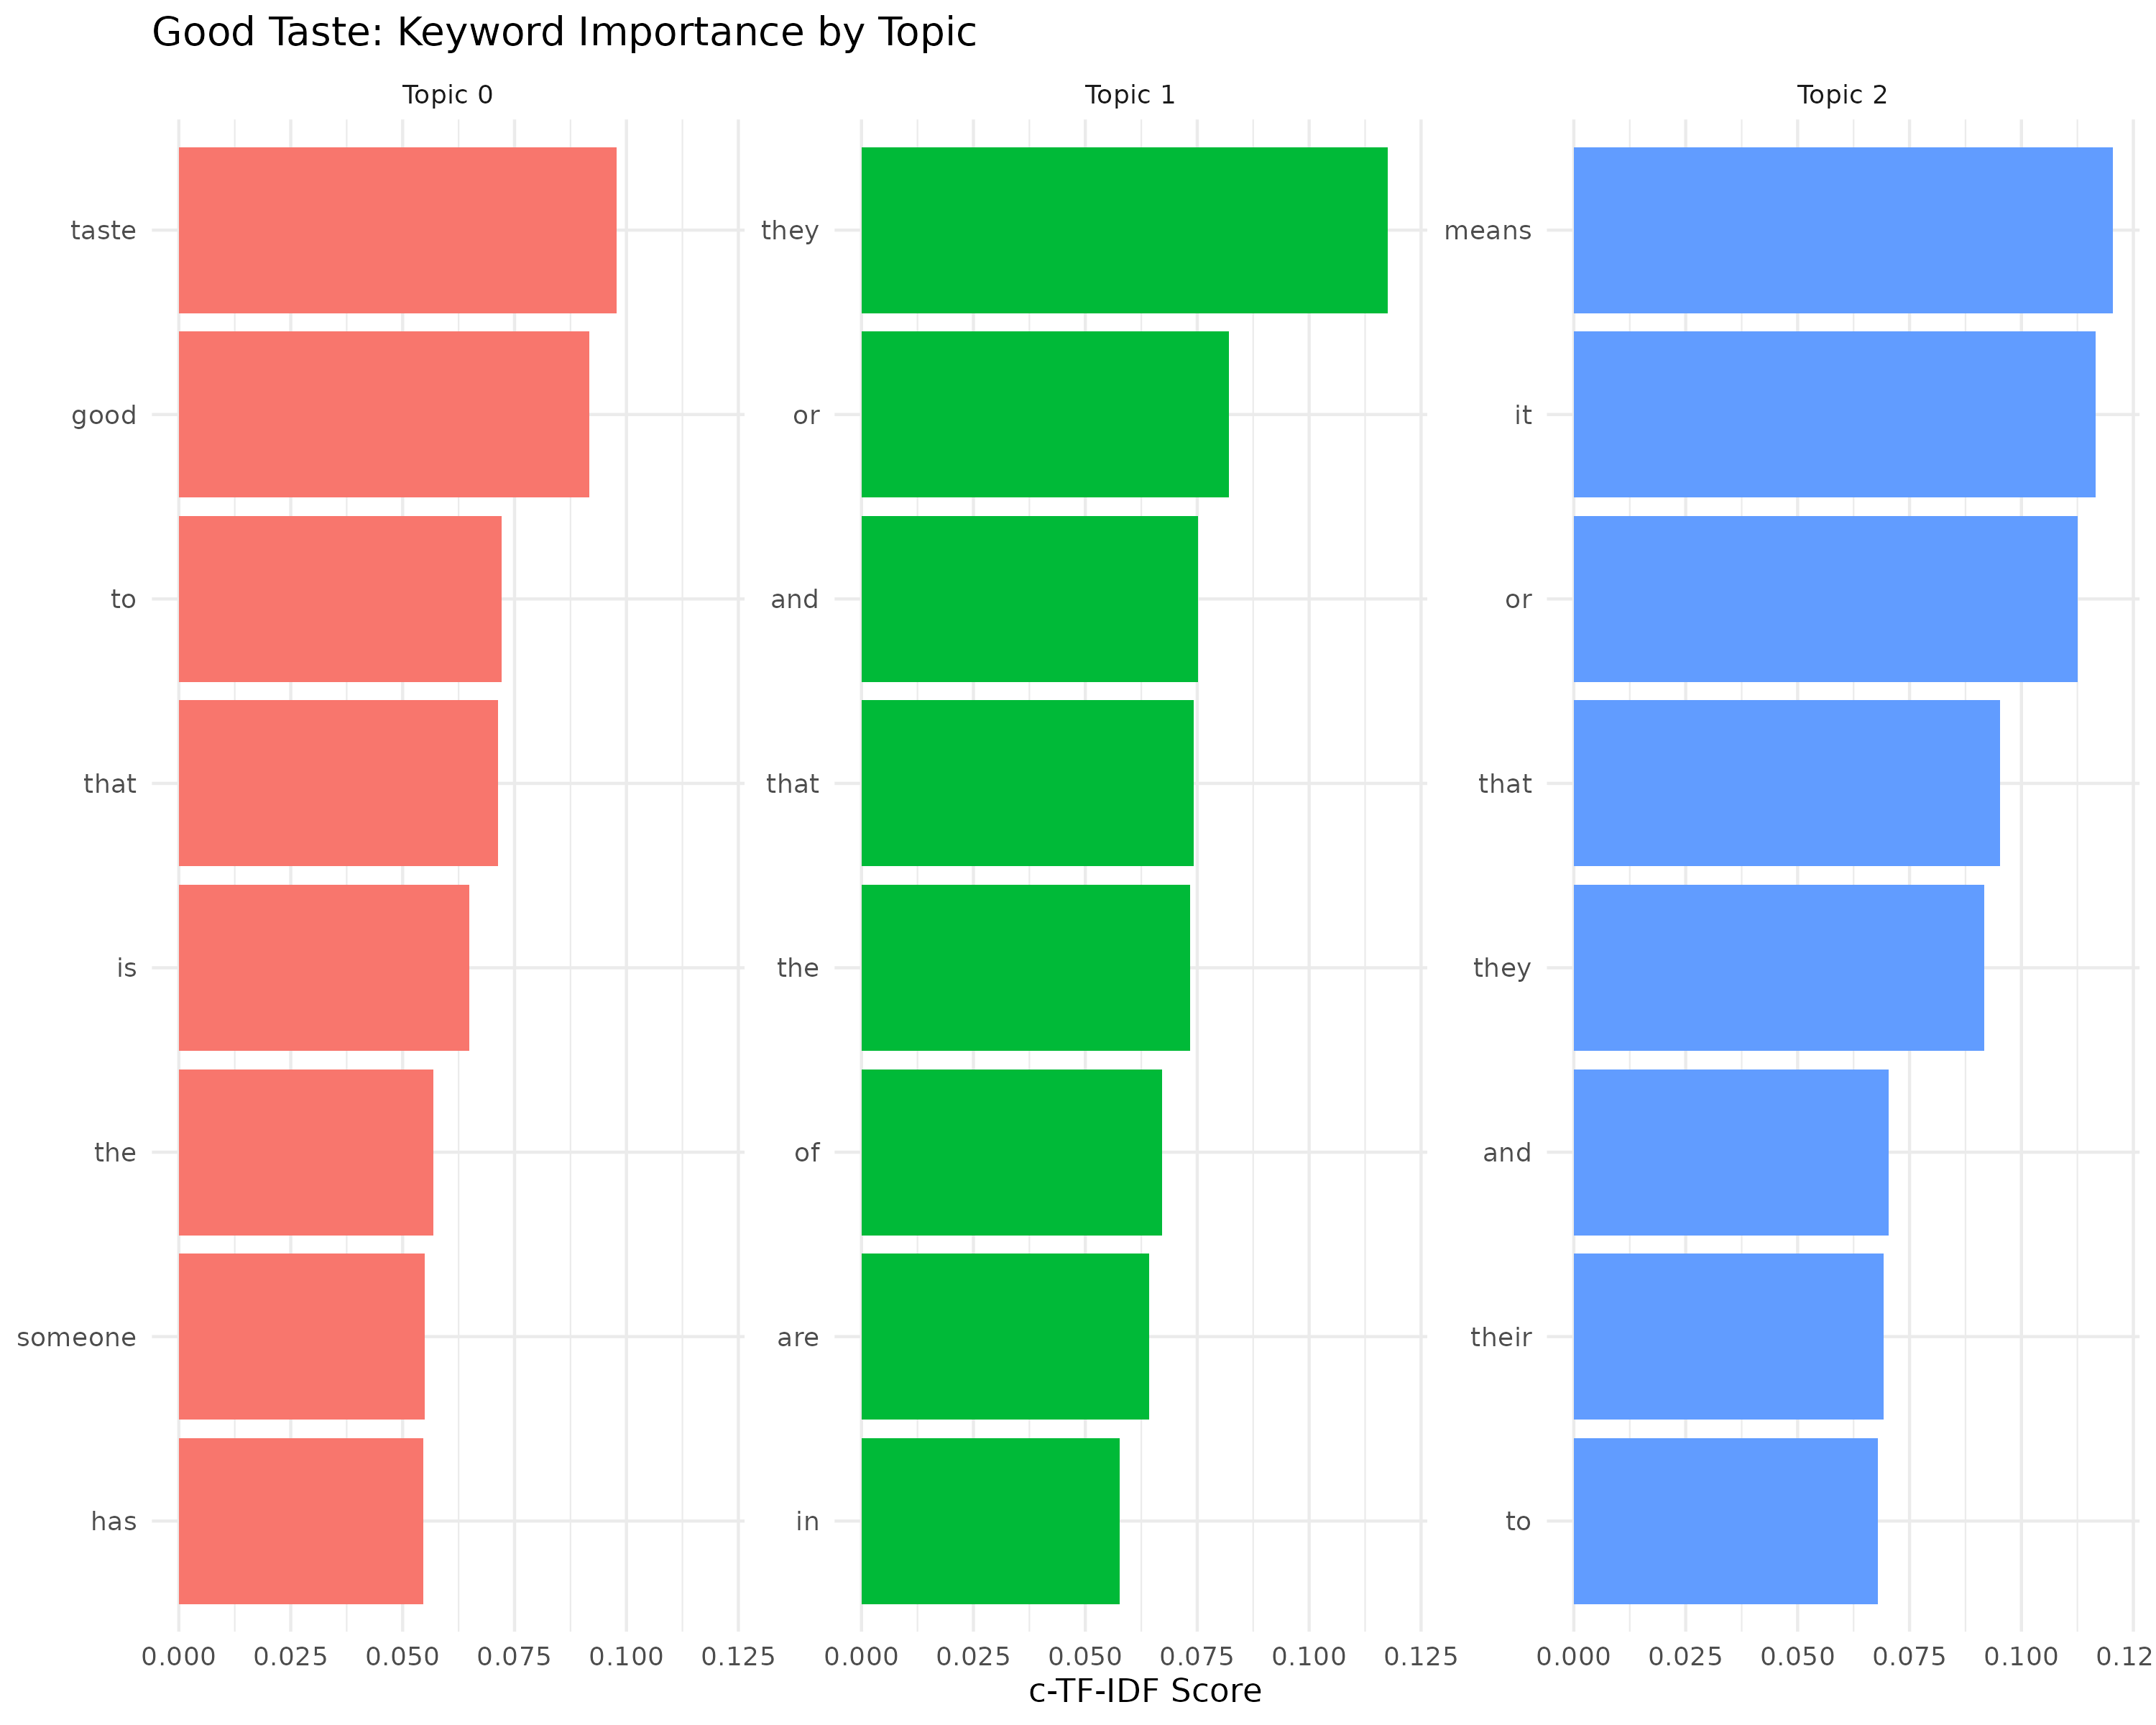
\includegraphics[width=\textwidth]{report/Plots/good_taste_keywords.png}
    \caption{Keyword Importance (c-TF-IDF) for Good Taste Topics (Definitions)}
    \label{fig:good_keywords_def}
\end{figure}

\begin{figure}[htpb]
    \centering
    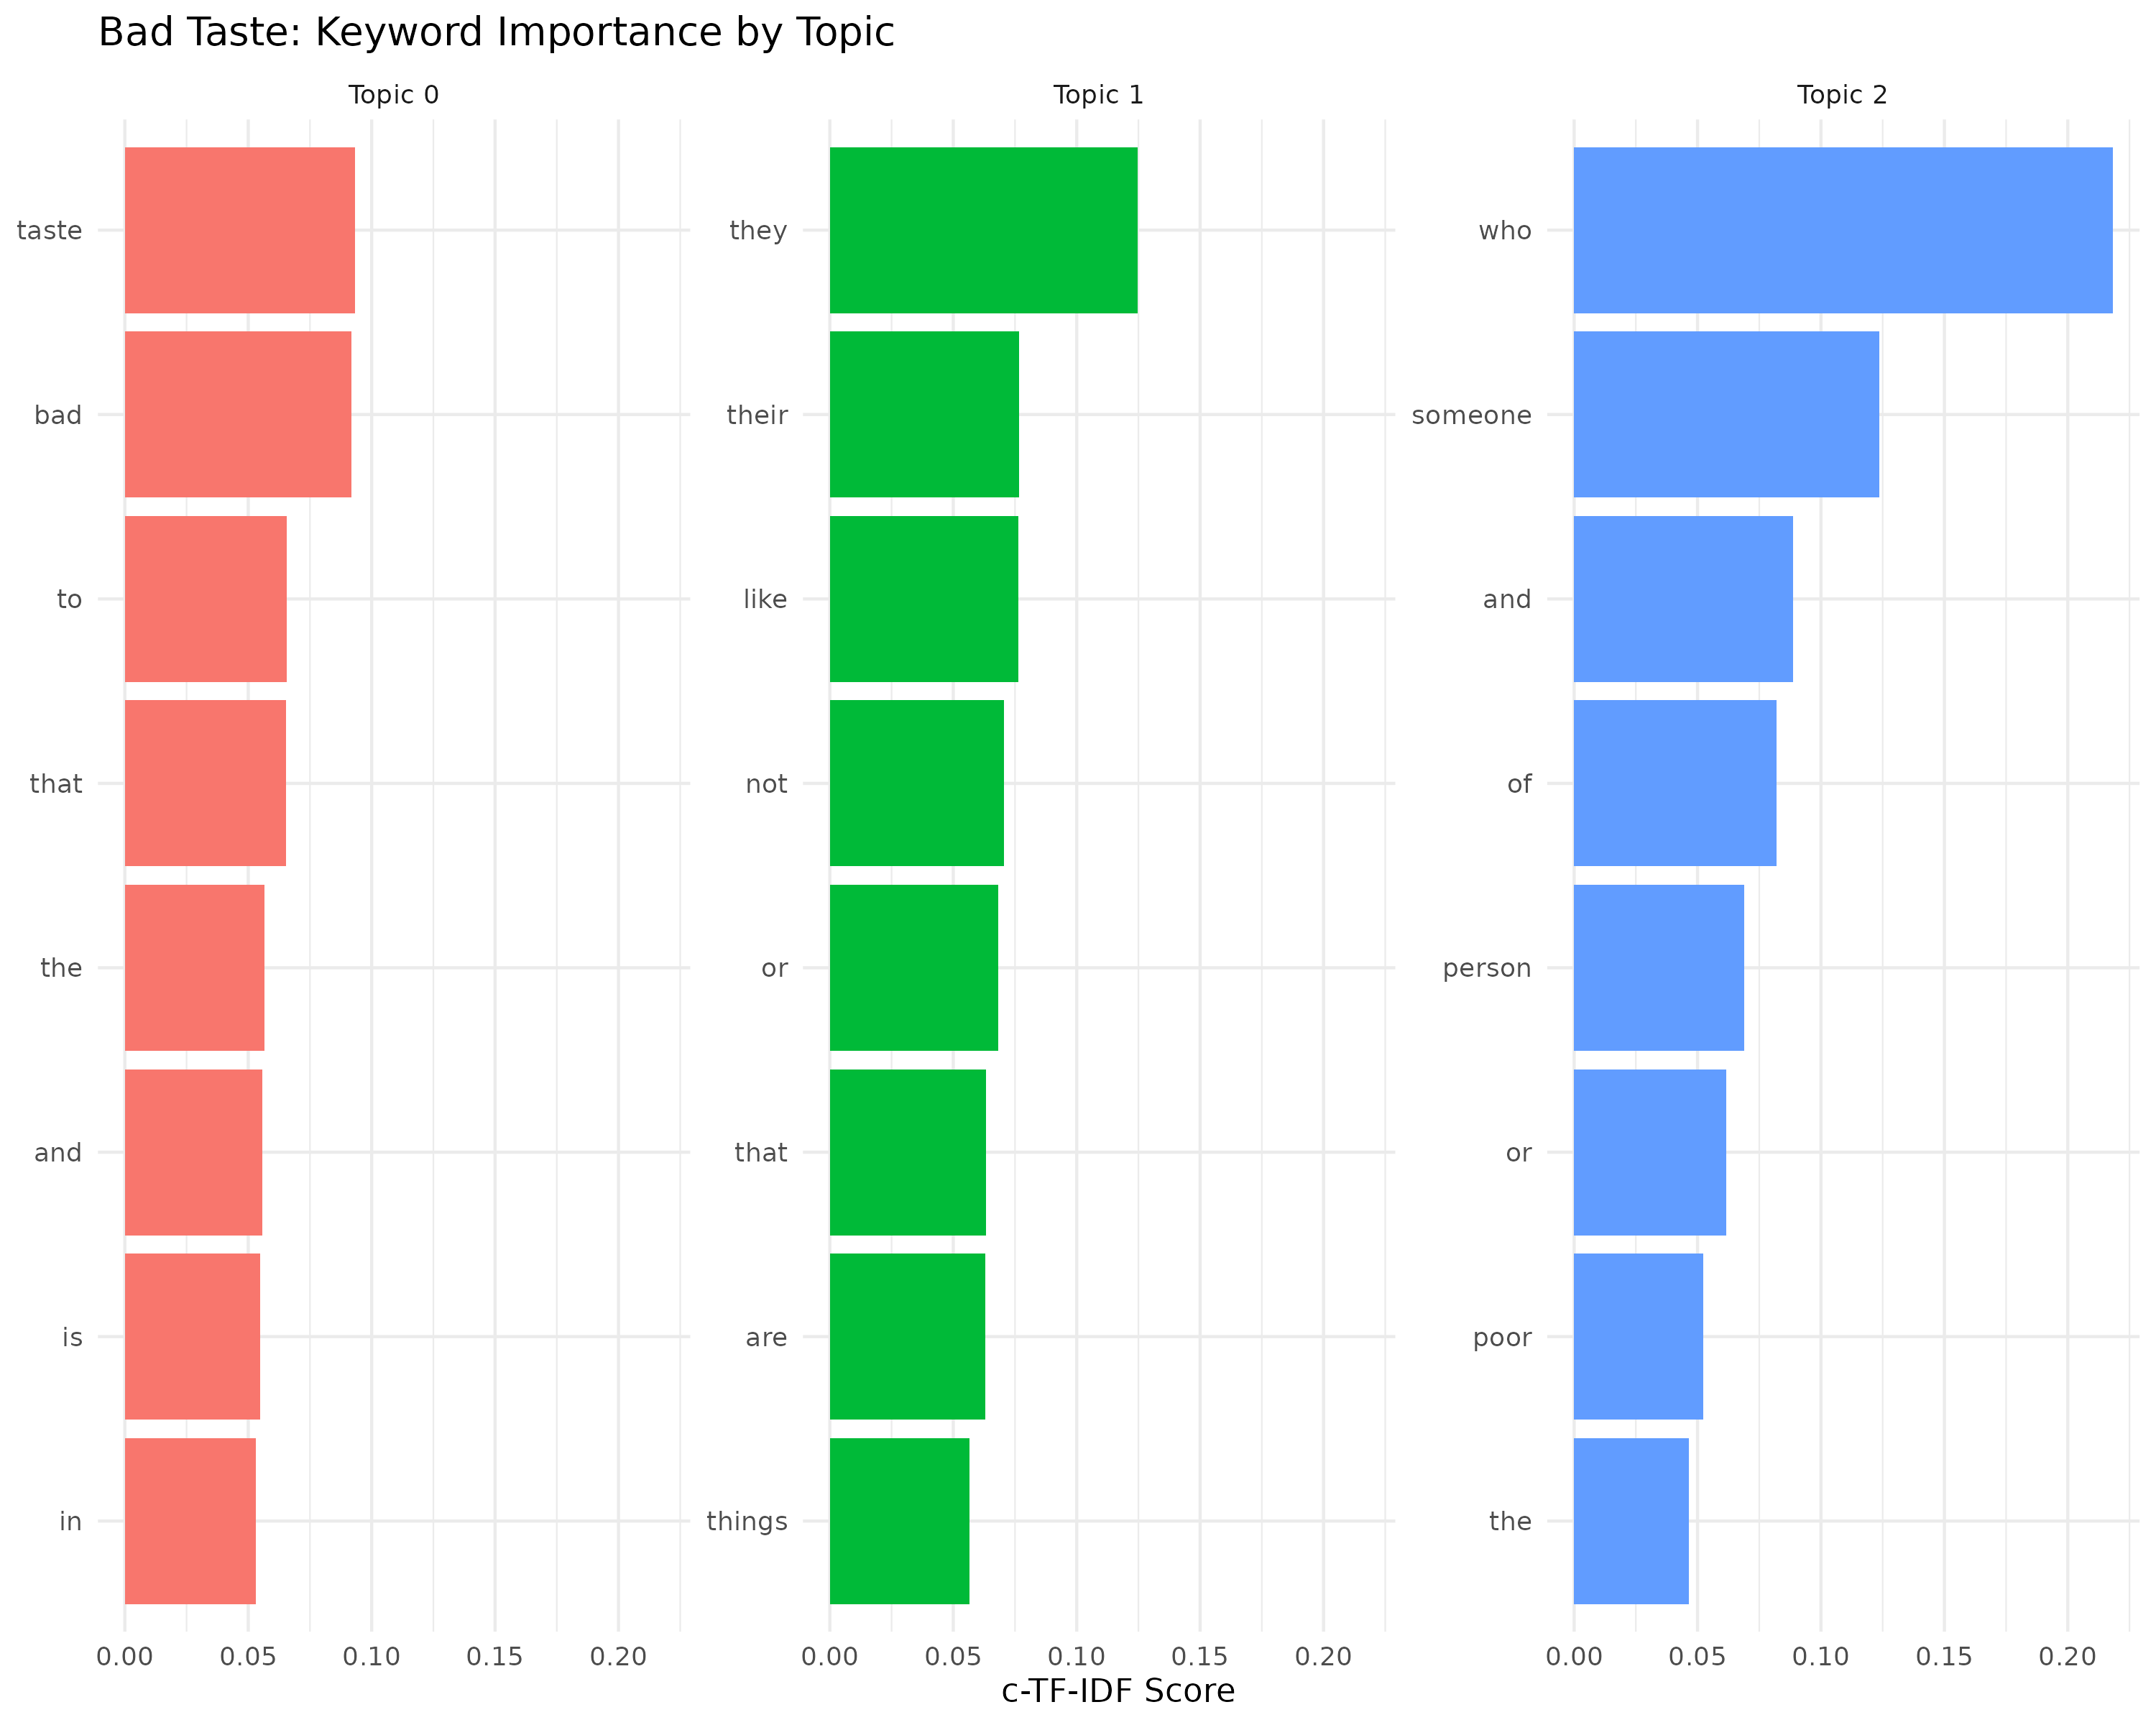
\includegraphics[width=\textwidth]{report/Plots/bad_taste_keywords.png}
    \caption{Keyword Importance (c-TF-IDF) for Bad Taste Topics (Definitions)}
    \label{fig:bad_keywords_def}
\end{figure}

\begin{figure}[htpb]
    \centering
    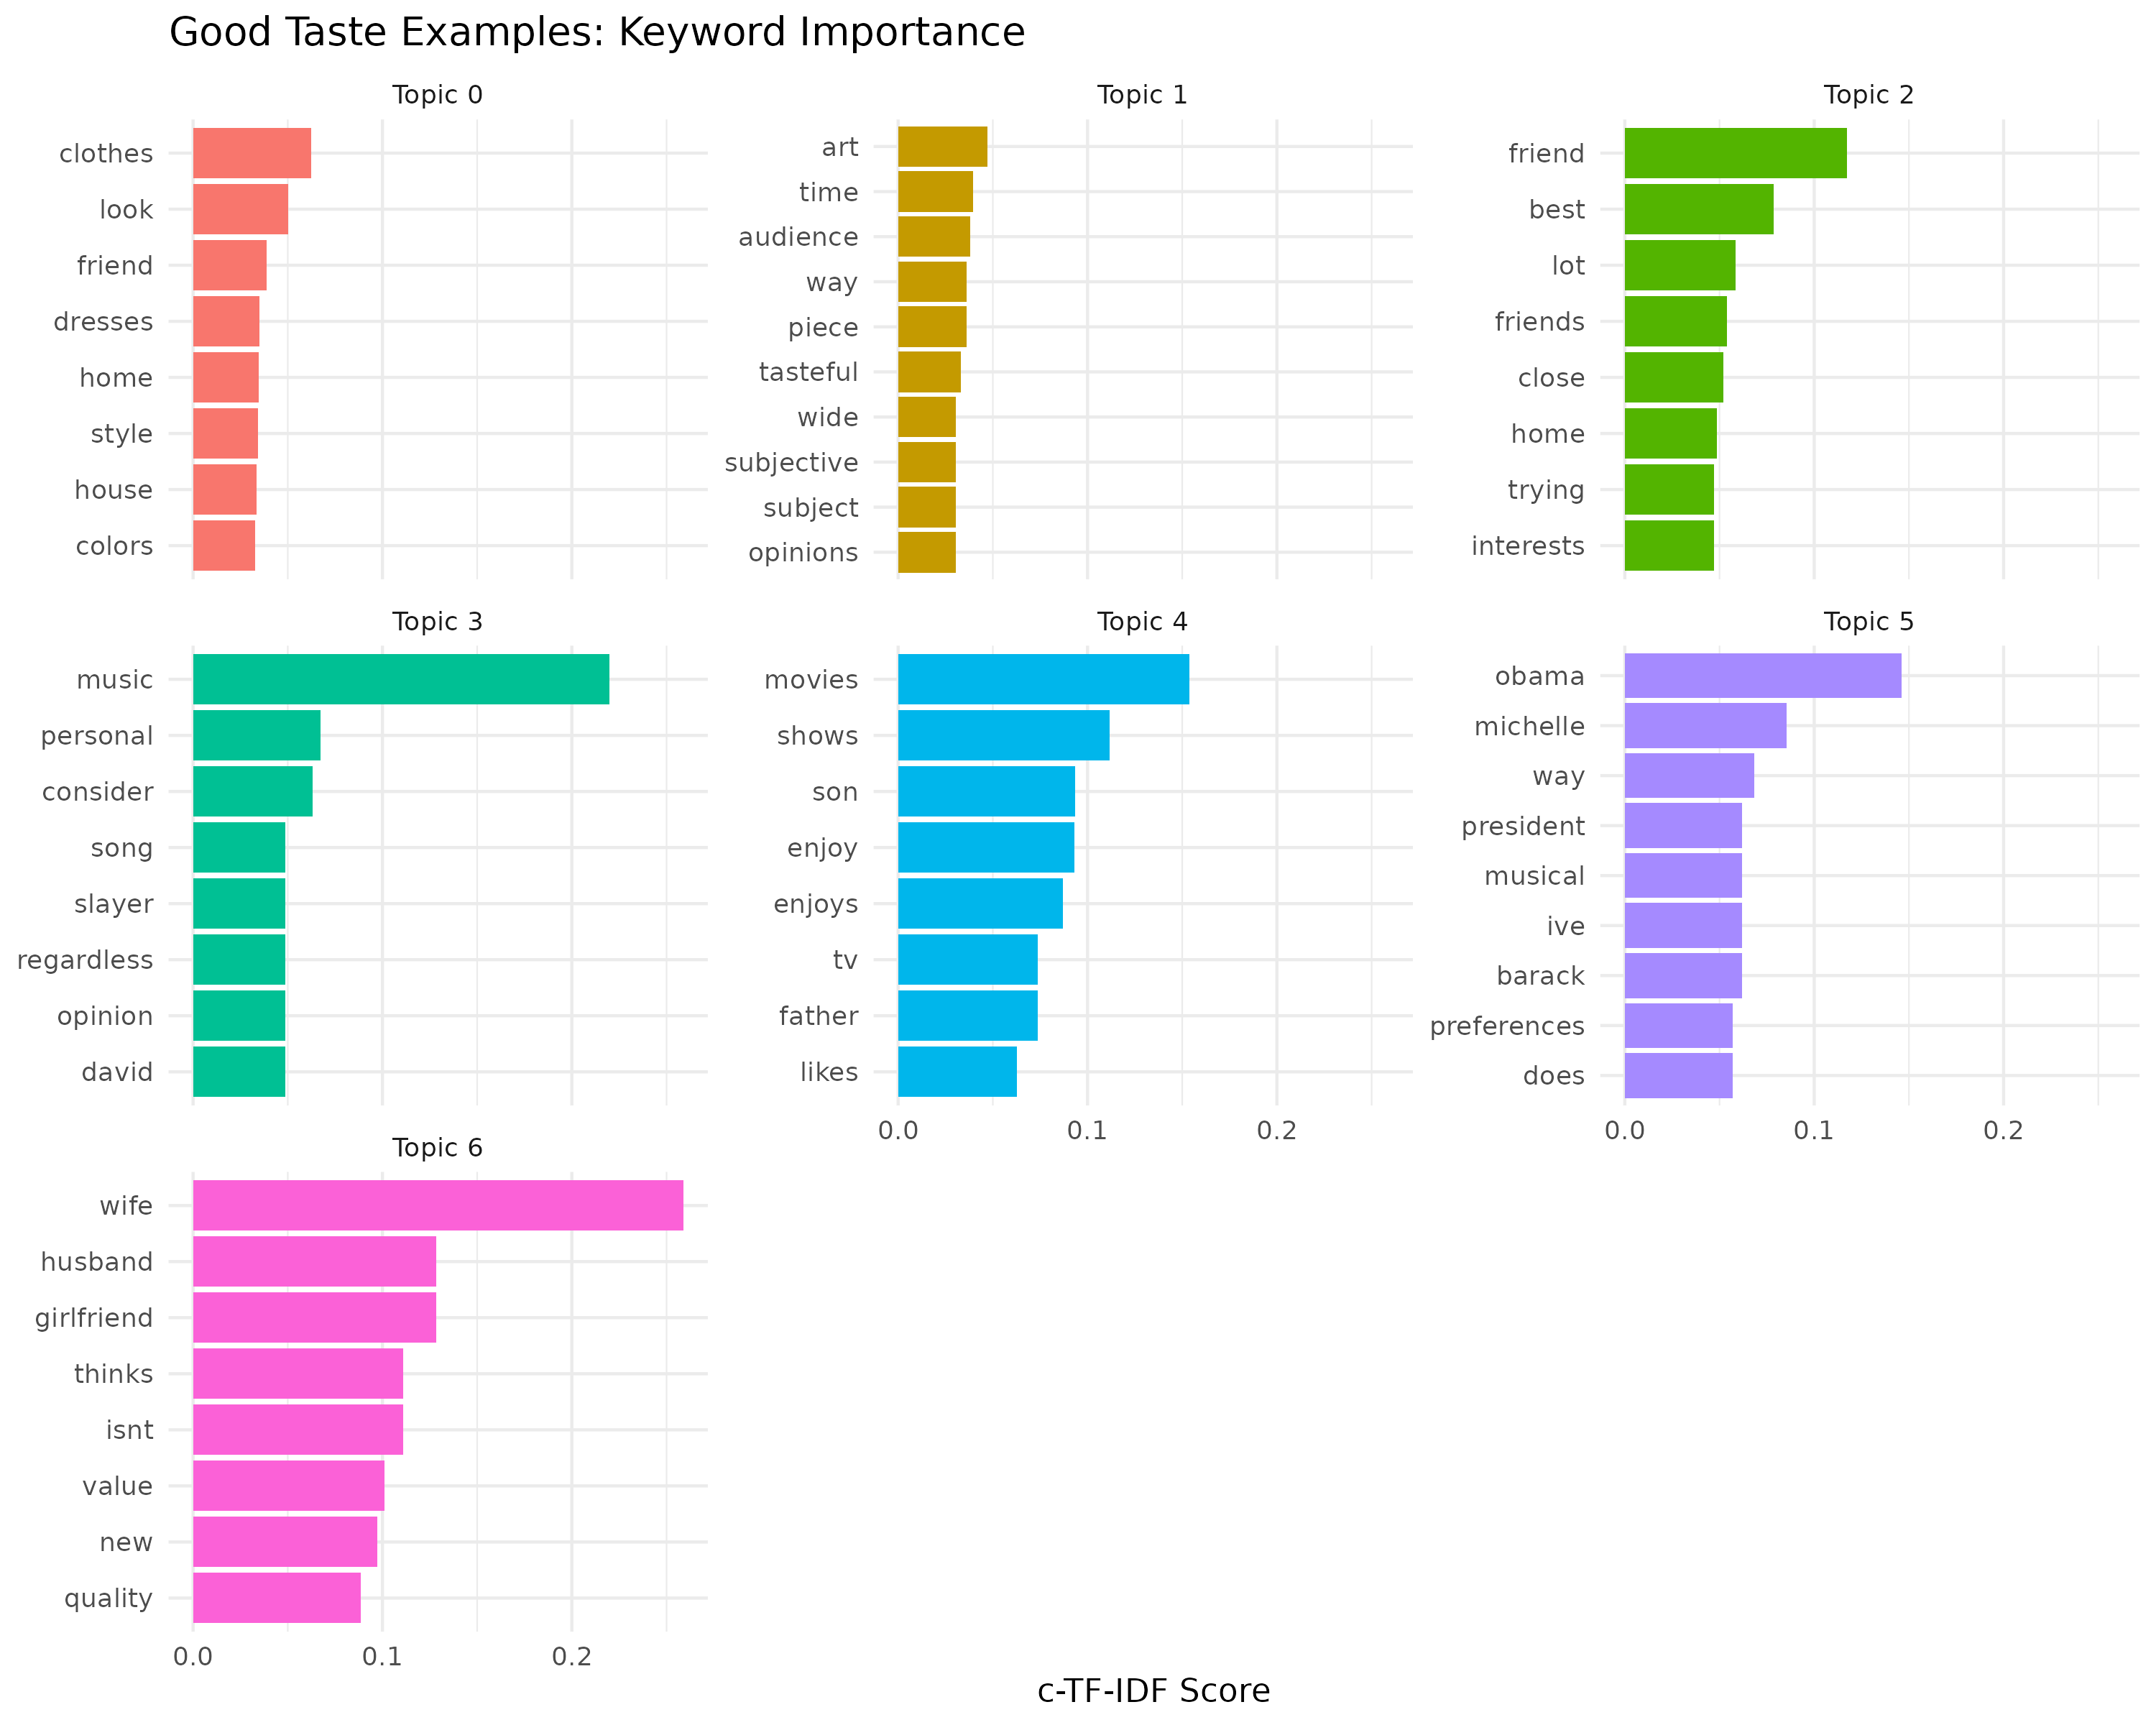
\includegraphics[width=\textwidth]{report/Plots/good_taste_example_keywords.png}
    \caption{Keyword Importance (c-TF-IDF) for Good Taste Topics (Examples)}
    \label{fig:good_keywords_ex}
\end{figure}

\begin{figure}[htpb]
    \centering
    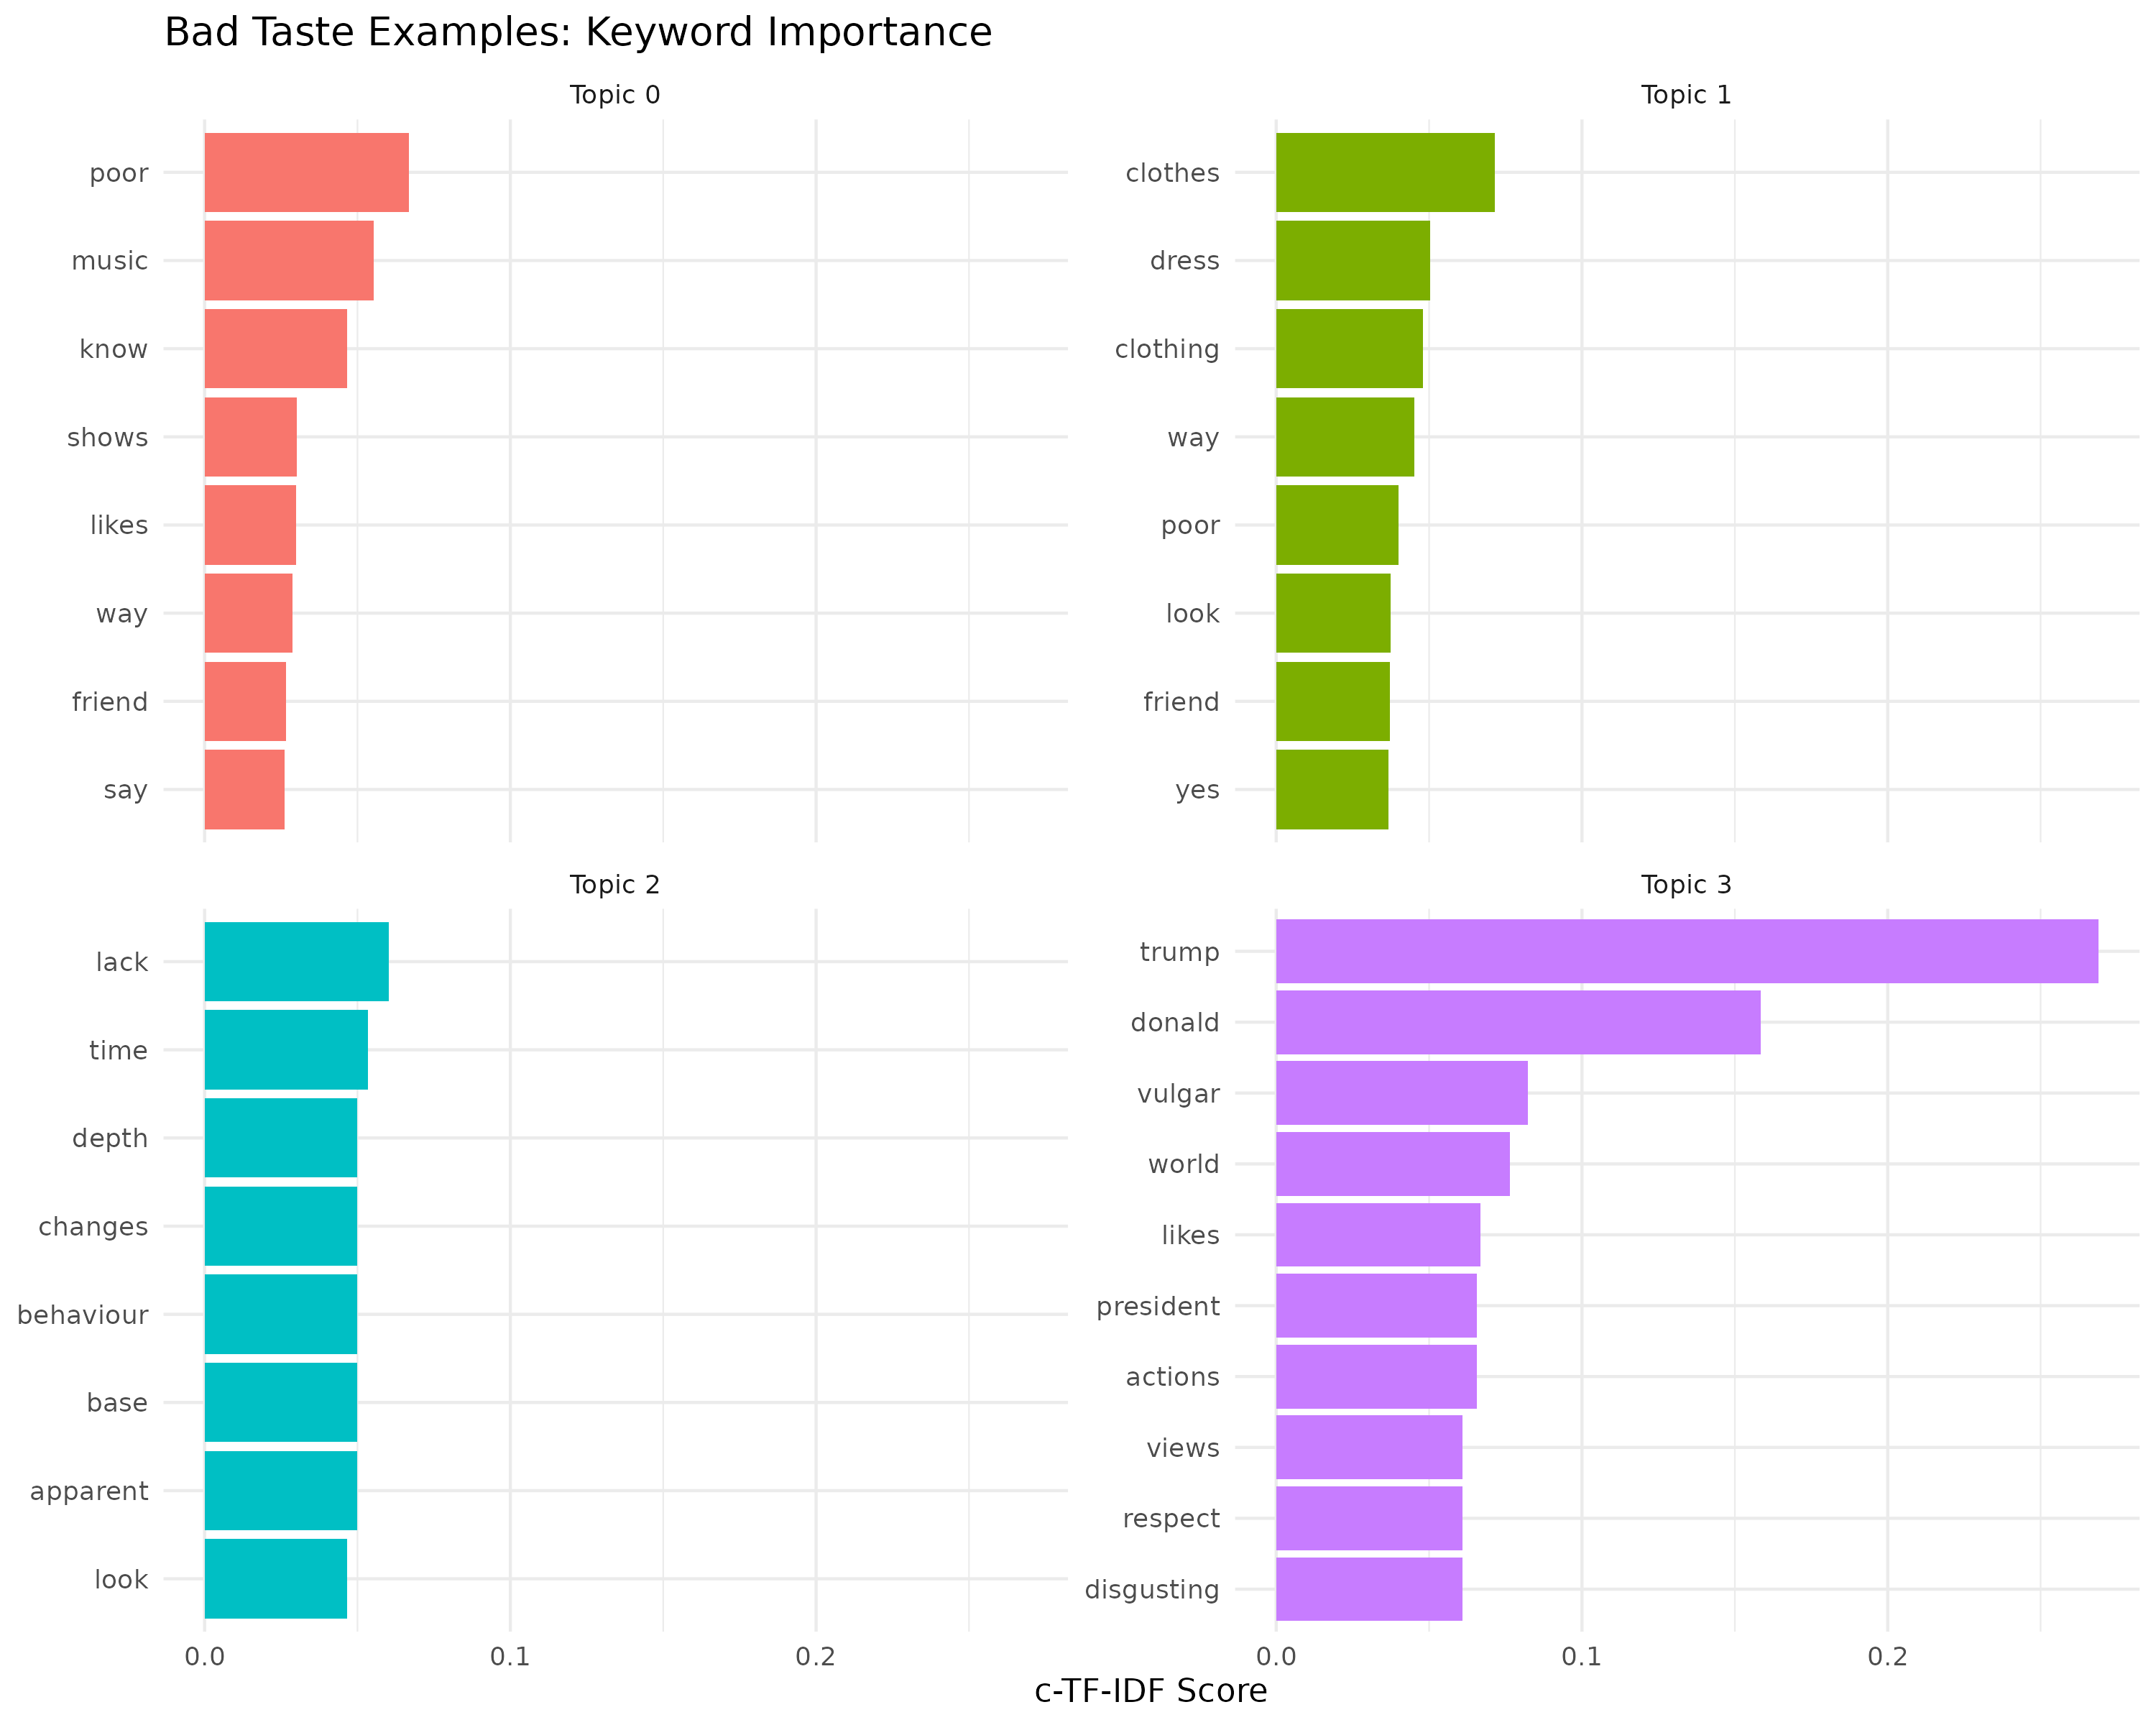
\includegraphics[width=\textwidth]{report/Plots/bad_taste_example_keywords.png}
    \caption{Keyword Importance (c-TF-IDF) for Bad Taste Topics (Examples)}
    \label{fig:bad_keywords_ex}
\end{figure}

\subsection{Cross-Schema Cultural Logics}

To test whether these cultural models are isolated or form coherent ``logics,'' I cross-tabulated respondents' primary cultural models across the four questions. The associations are highly significant. For instance, a respondent's definition of Good Taste strongly predicts their definition of Bad Taste ($\chi^2 = 111.60, p < 0.001$). Individuals who define good taste as subjective similarity overwhelmingly define bad taste simply as subjective dislike. 

Similarly, the examples respondents choose are highly correlated ($\chi^2 = 99.01, p < 0.001$). Respondents who cite a friend's ``Fashion/Decor'' as an example of good taste are highly likely to cite ``Poor Fashion'' as an example of bad taste. Respondents who point to ``Refinement/Art'' for good taste are much more likely to point to ``Derivative Media'' for bad taste. This symmetry indicates that people deploy consistent criteria---whether aesthetic, material, or subjective---across moral valences.

\begin{figure}[htpb]
    \centering
    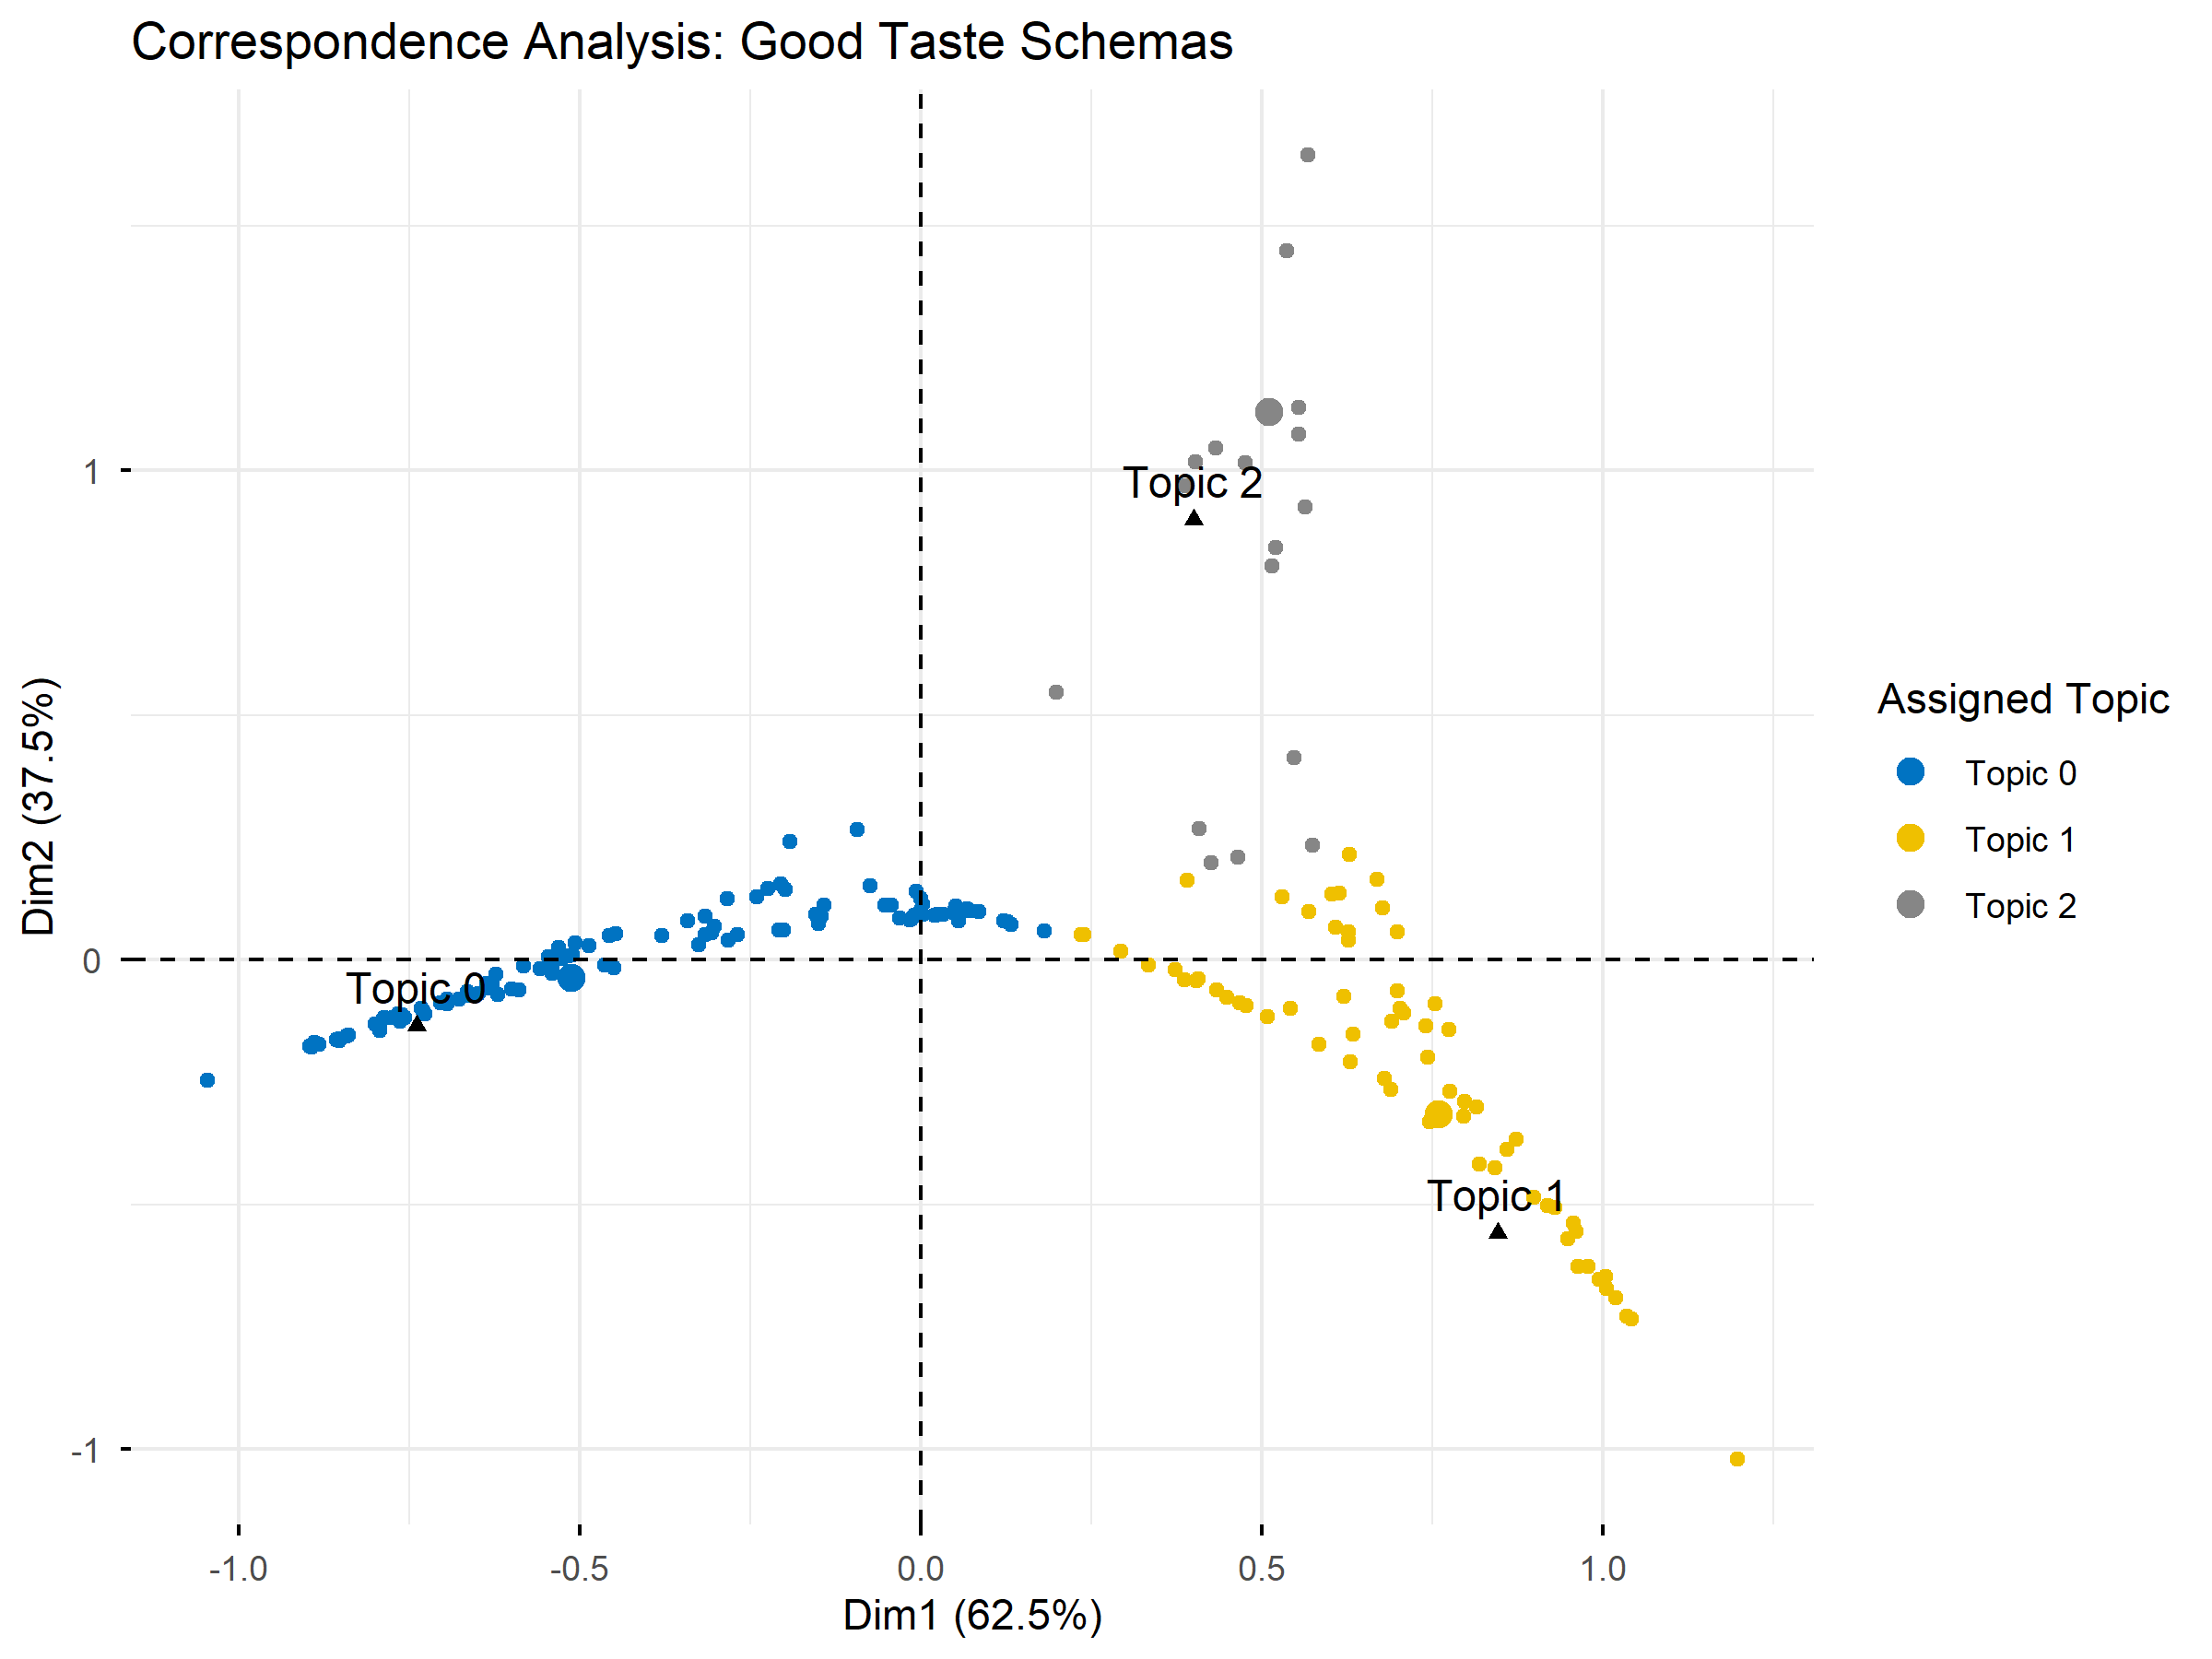
\includegraphics[width=0.48\textwidth]{report/Plots/ca_good_taste.png}
    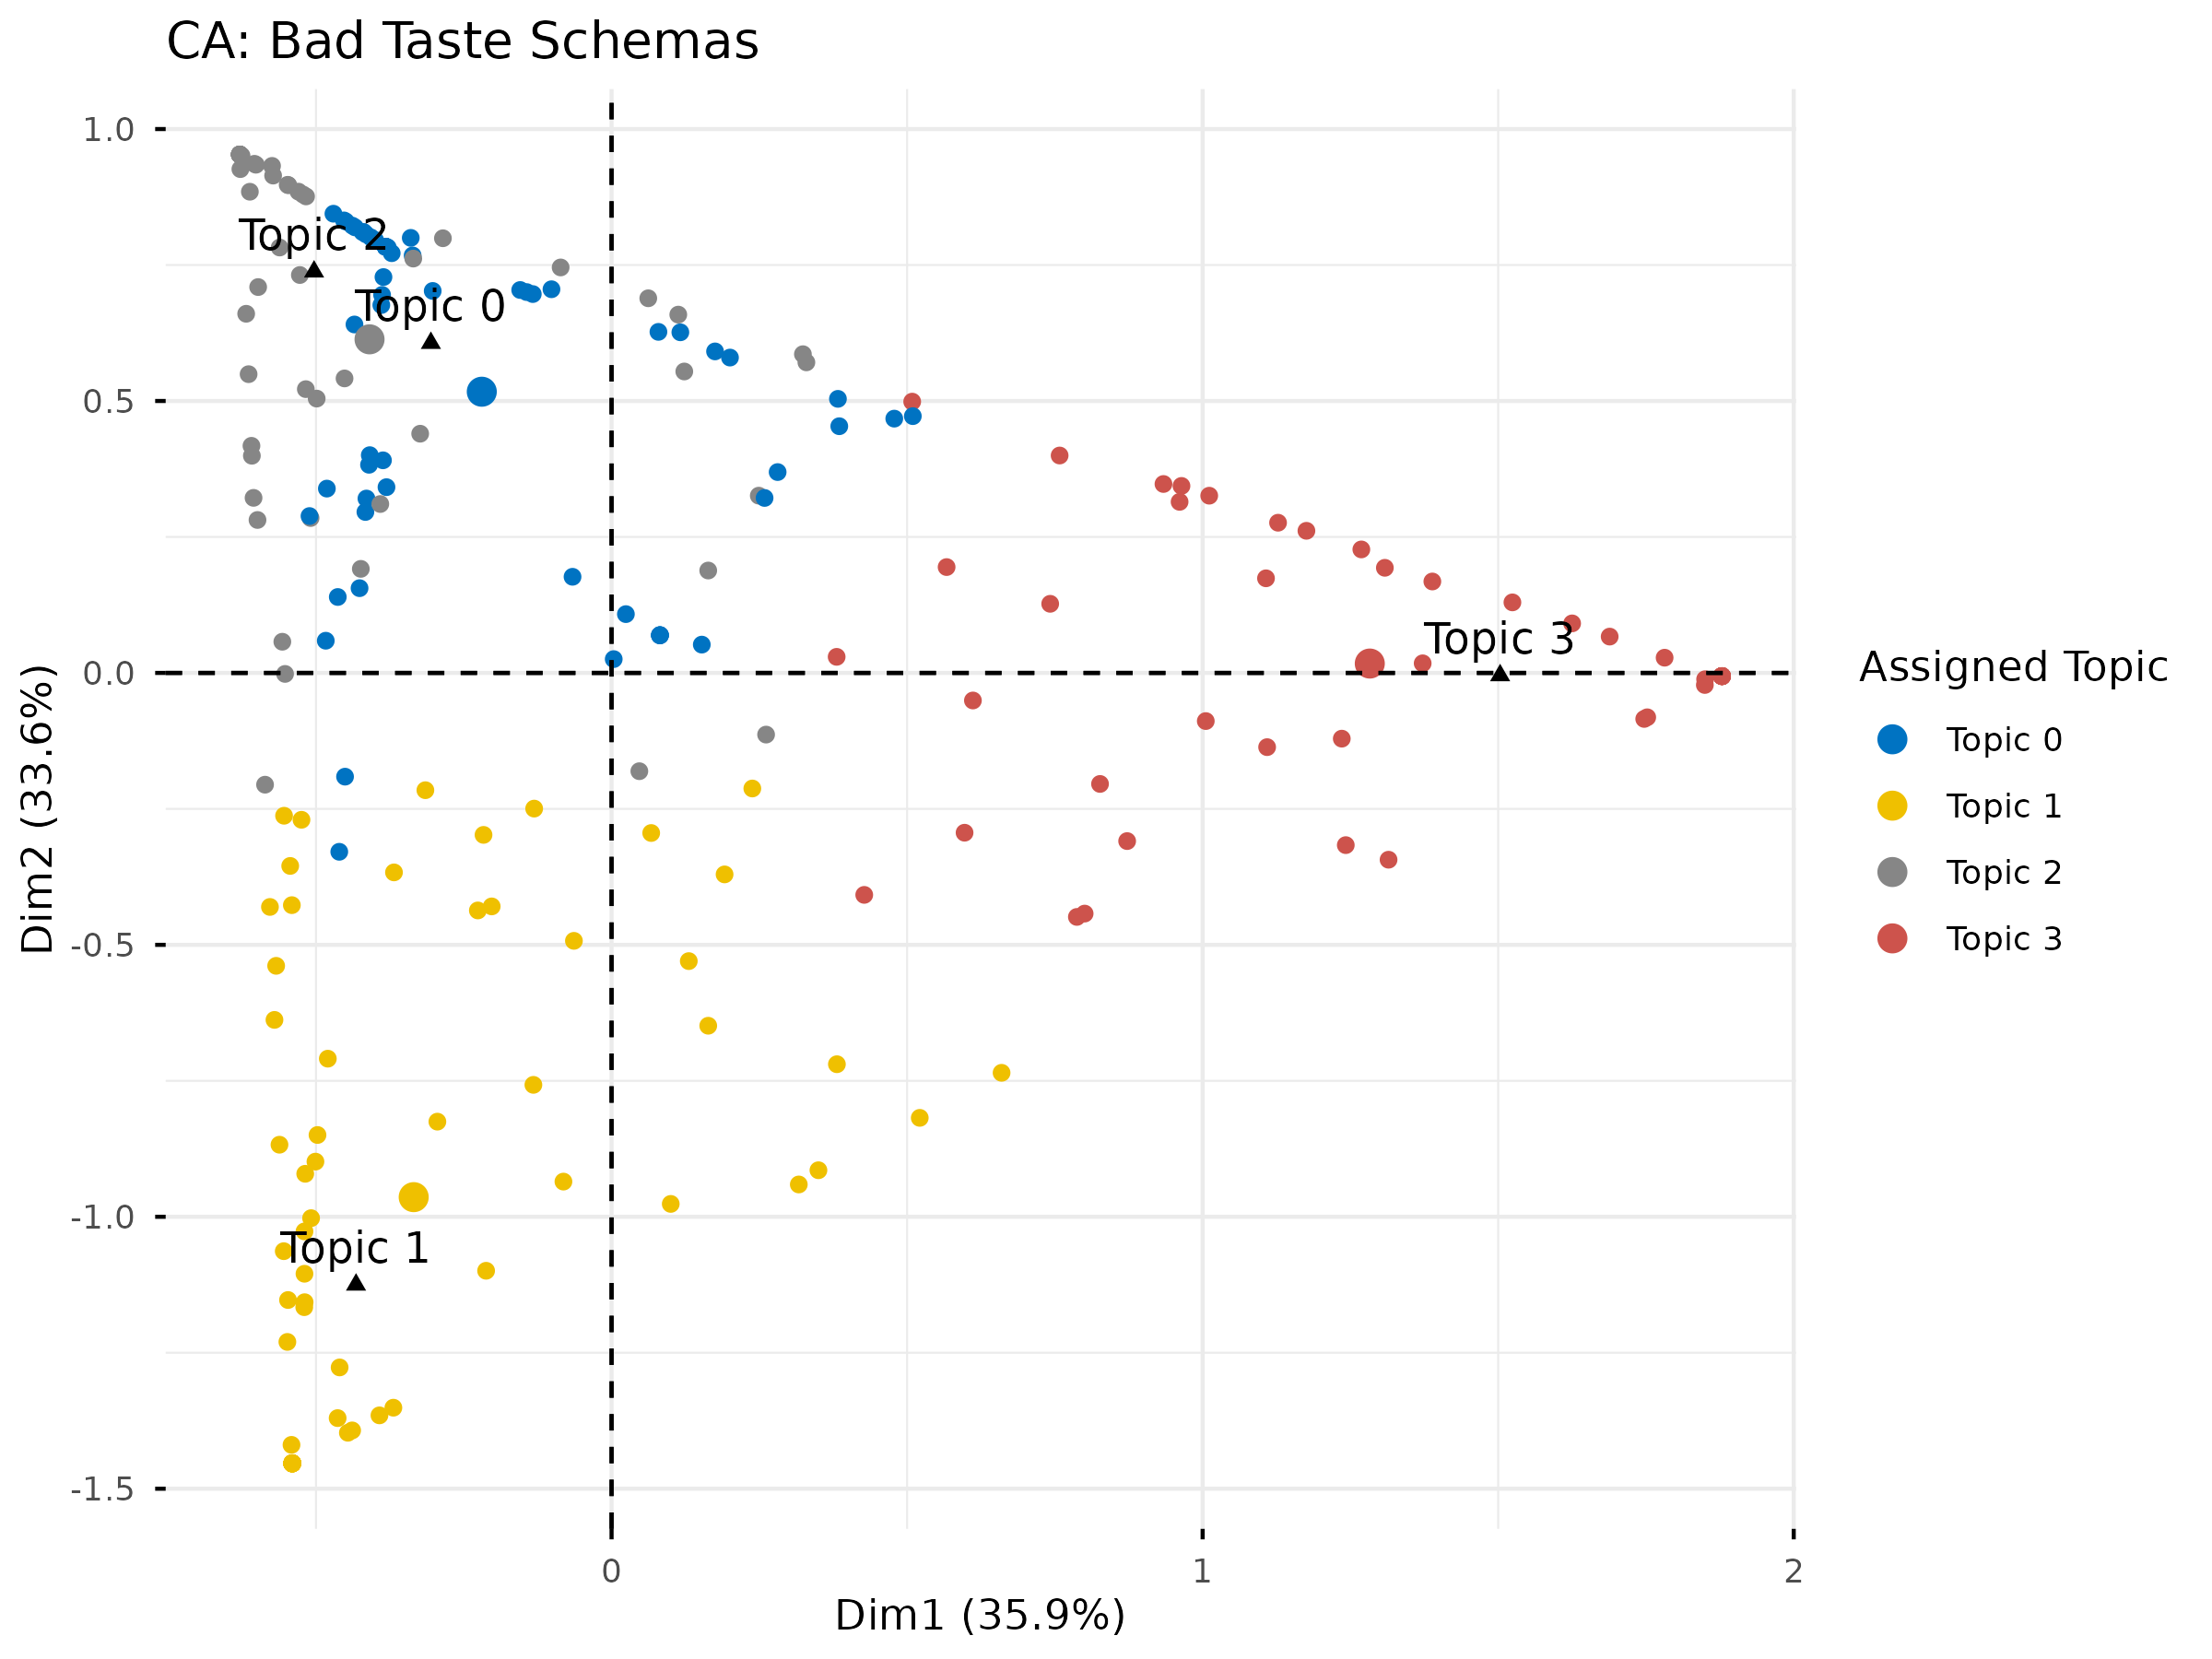
\includegraphics[width=0.48\textwidth]{report/Plots/ca_bad_taste.png}
    \caption{Correspondence Analysis of Taste Schemas (Definitions)}
    \label{fig:ca_schemas_def}
\end{figure}

\begin{figure}[htpb]
    \centering
    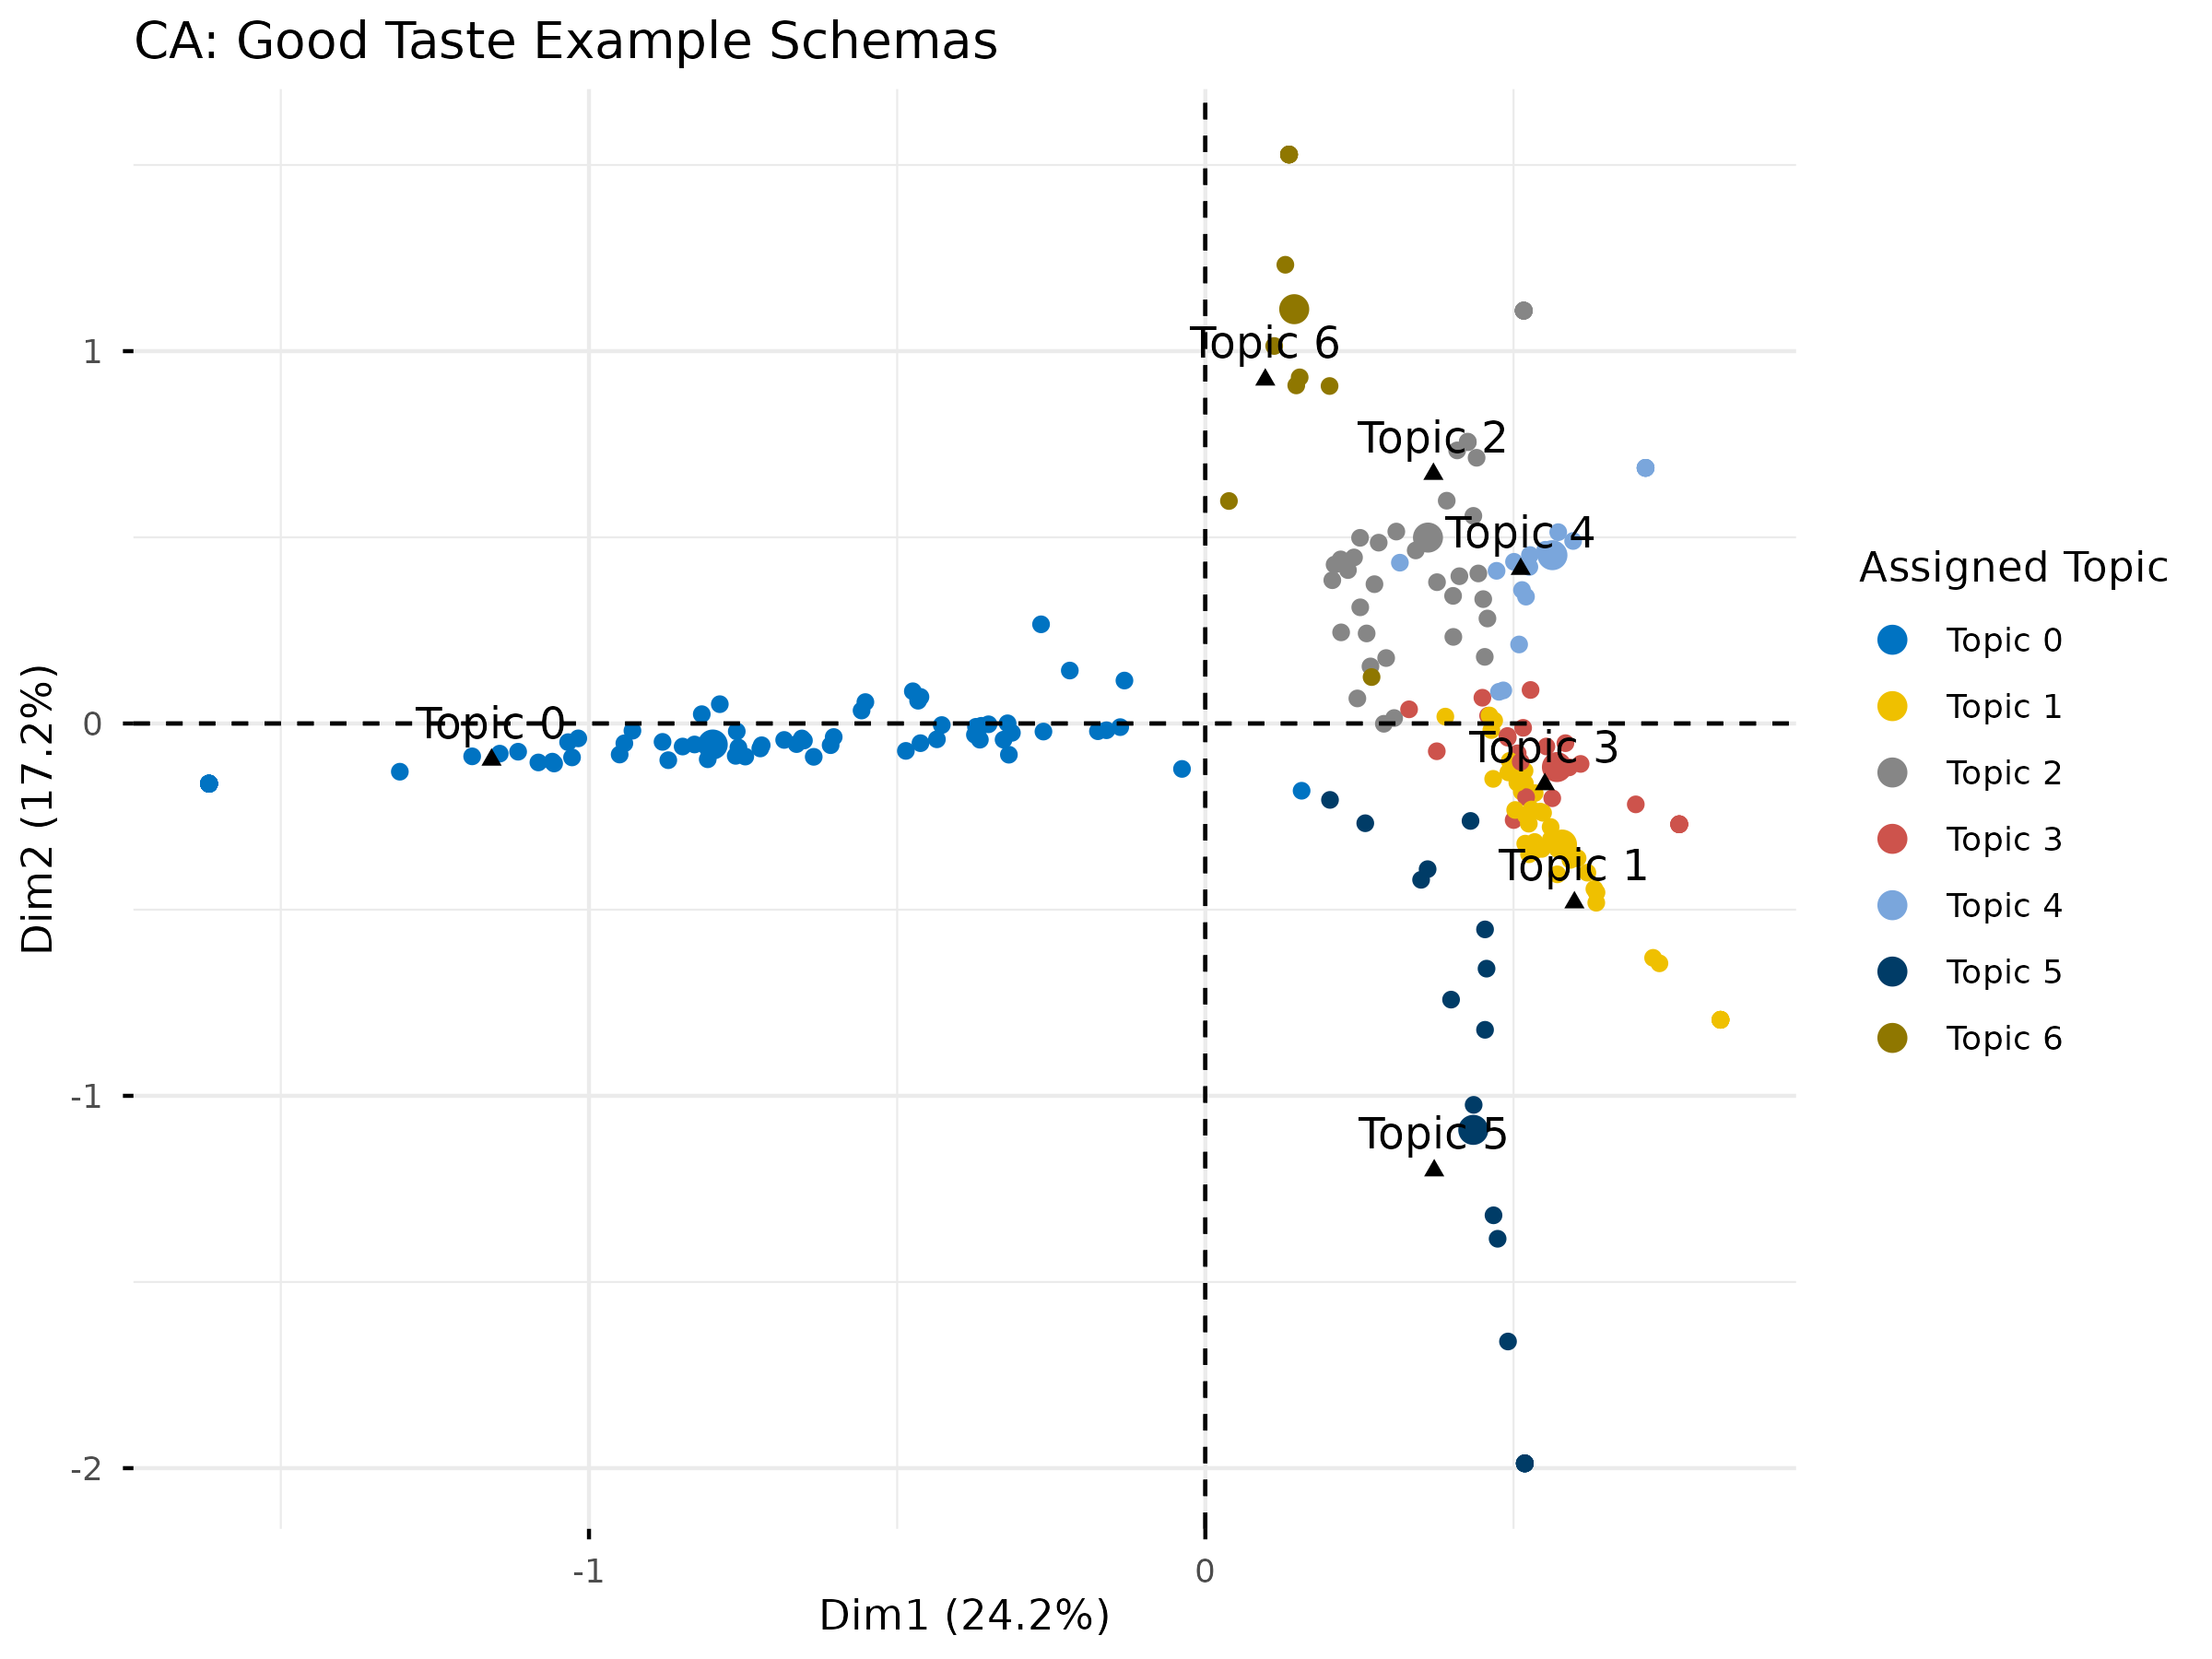
\includegraphics[width=0.48\textwidth]{report/Plots/ca_good_taste_example.png}
    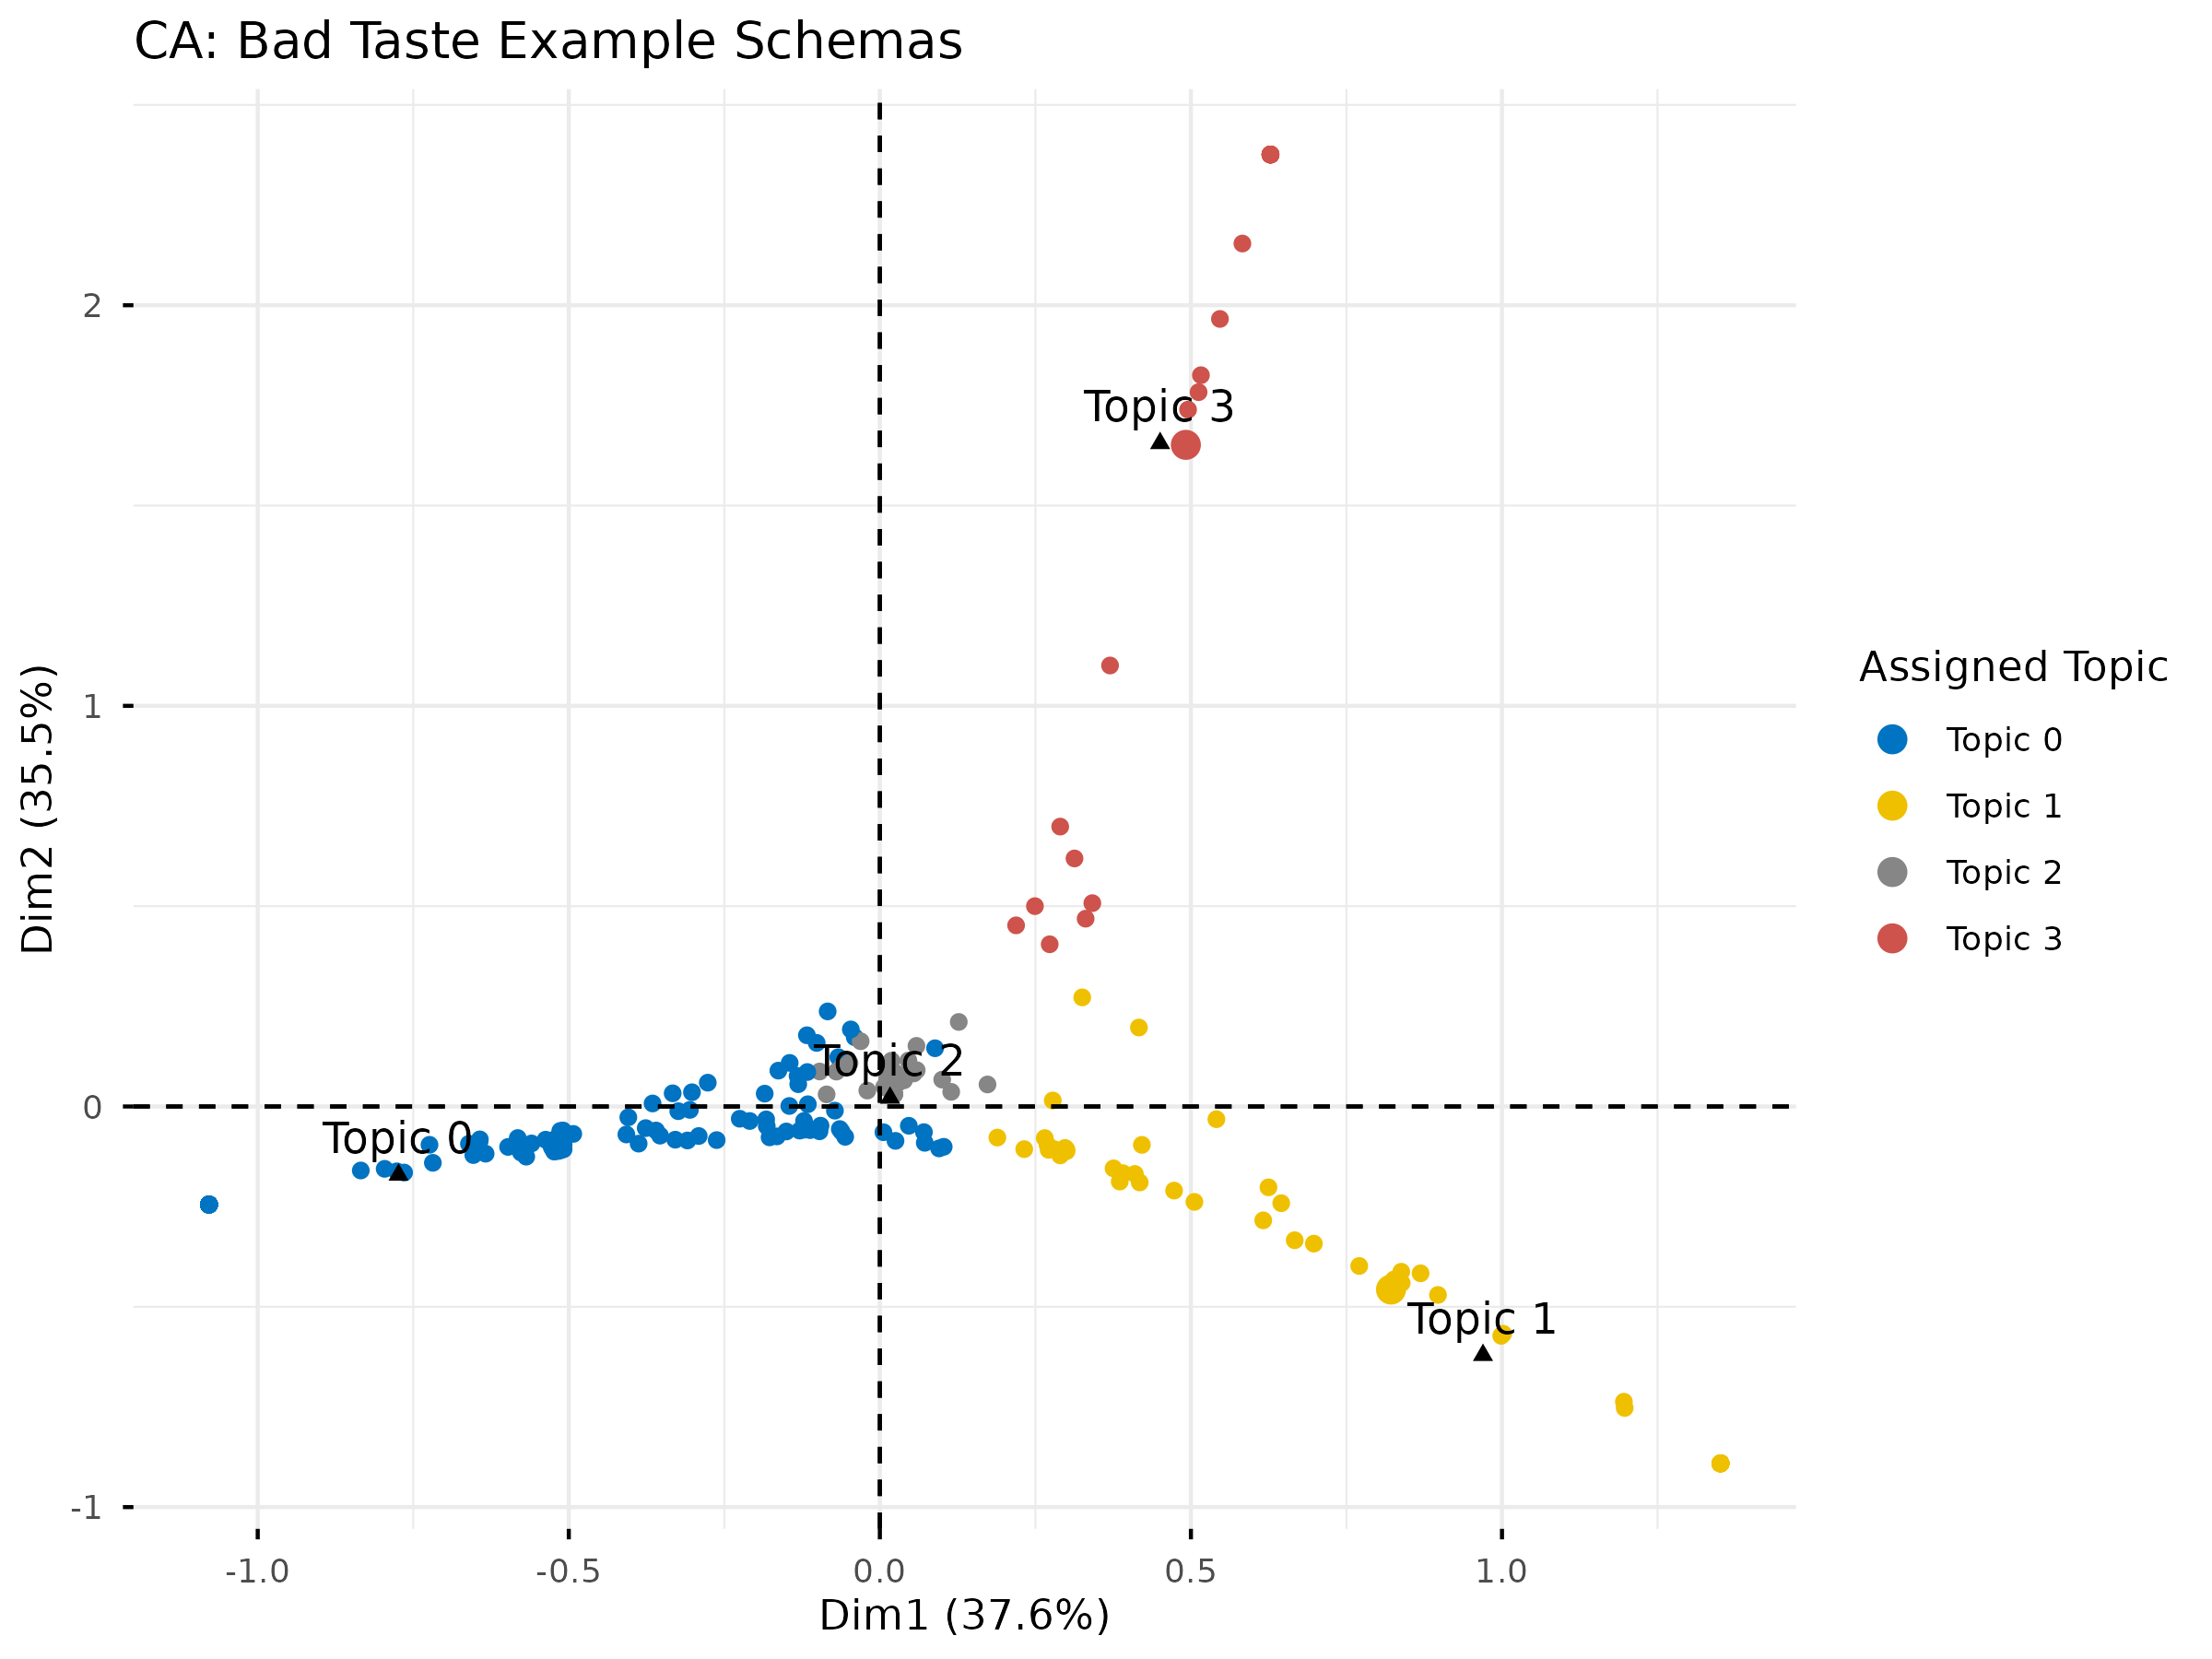
\includegraphics[width=0.48\textwidth]{report/Plots/ca_bad_taste_example.png}
    \caption{Correspondence Analysis of Taste Schemas (Examples)}
    \label{fig:ca_schemas_ex}
\end{figure}

\begin{figure}[htpb]
    \centering
    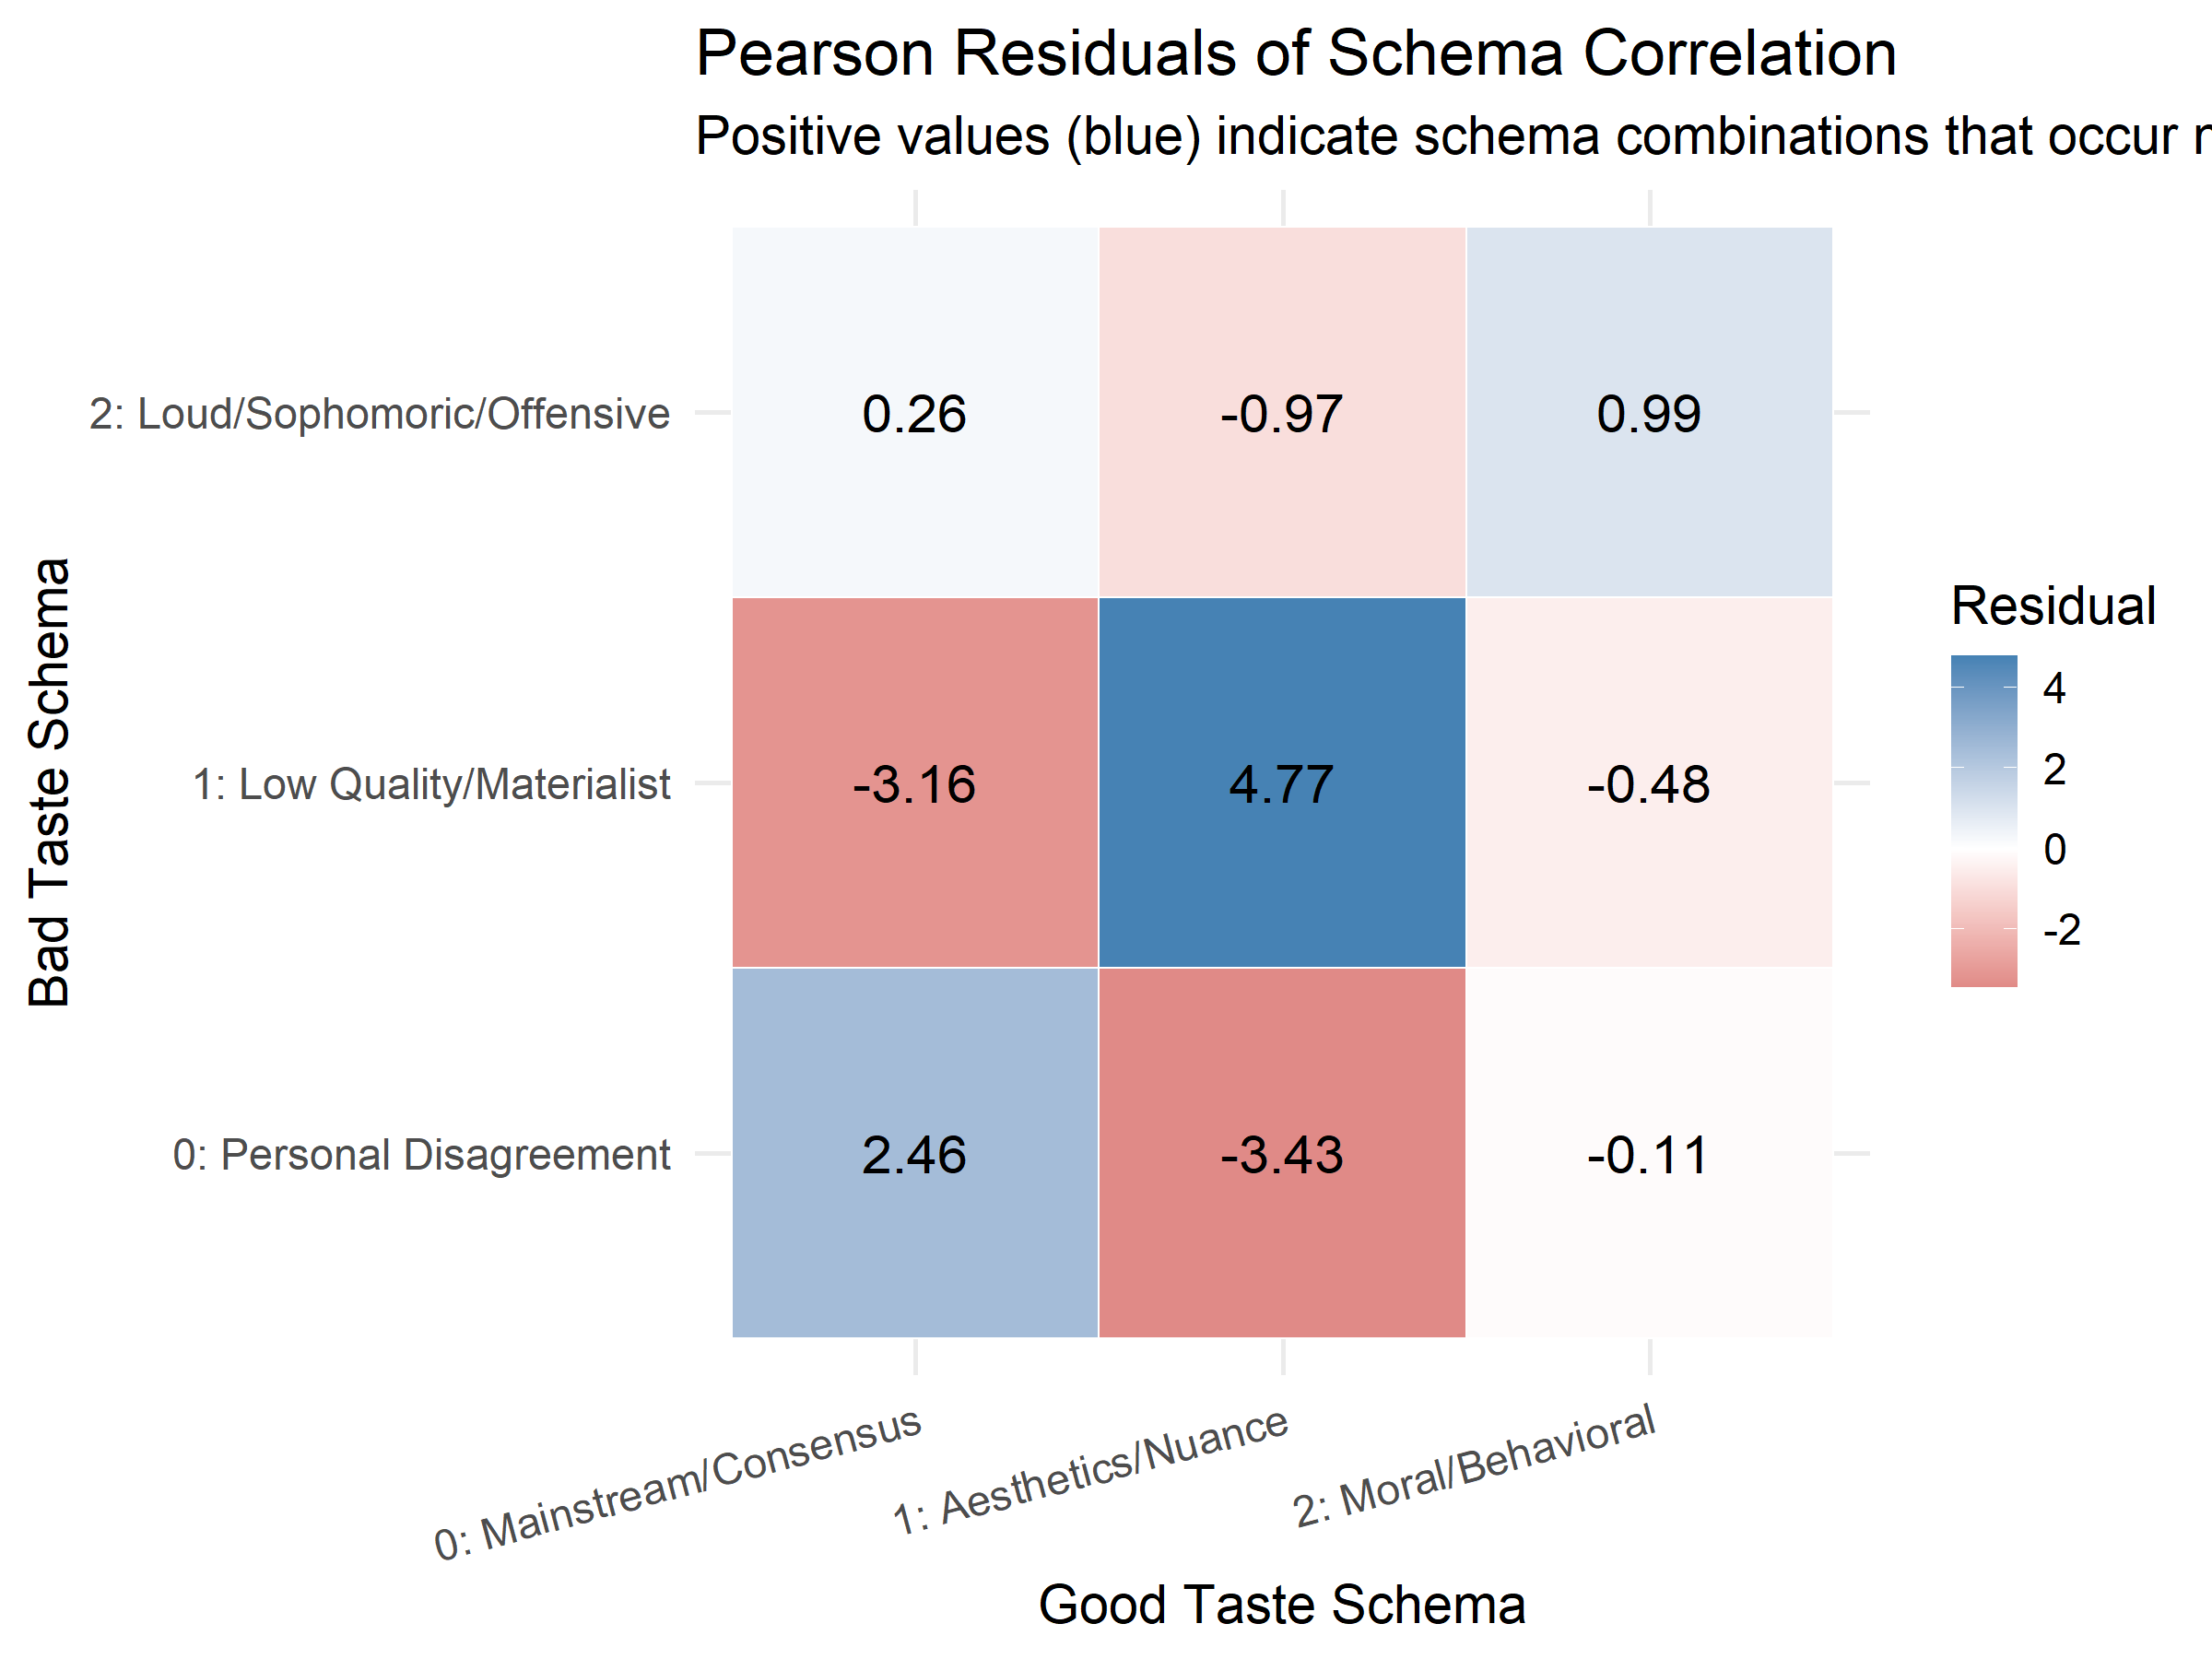
\includegraphics[width=0.8\textwidth]{report/Plots/schema_correlation.png}
    \caption{Pearson Residuals of Schema Correlation}
    \label{fig:schema_corr}
\end{figure}

\subsection{Demographics}

\begin{table}[htpb]
\centering
\resizebox{\textwidth}{!}{
\begin{tabular}{llrrr}
\toprule
Model & Predictor & Wald $\chi^2$ & Df & $p$-value \\
\midrule
Good Taste Def & Age & 8.16 & 5 & 0.1479 \\
Good Taste Def & Gender & 3.40 & 5 & 0.6380 \\
Good Taste Def & EducationLevel\_Coded & 5.71 & 5 & 0.3351 \\
Good Taste Def & Political & 3.33 & 5 & 0.6493 \\
Bad Taste Def & Age & 4.02 & 2 & 0.1337 \\
Bad Taste Def & Gender & 0.53 & 2 & 0.7676 \\
Bad Taste Def & EducationLevel\_Coded & 0.56 & 2 & 0.7575 \\
Bad Taste Def & Political & 2.04 & 2 & 0.3614 \\
Good Taste Example & Age & 9.08 & 4 & 0.0590 \\
Good Taste Example & Gender & 5.02 & 4 & 0.2857 \\
Good Taste Example & EducationLevel\_Coded & 6.10 & 4 & 0.1916 \\
Good Taste Example & Political & 5.54 & 4 & 0.2364 \\
Bad Taste Example & Age & 6.43 & 3 & 0.0925 \\
Bad Taste Example & Gender & 0.74 & 3 & 0.8642 \\
Bad Taste Example & EducationLevel\_Coded & 2.22 & 3 & 0.5283 \\
Bad Taste Example & Political & 3.29 & 3 & 0.3491 \\
\bottomrule
\end{tabular}
}
\caption{Multinomial Logistic Regression Wald Tests for Topic Predictors}
\label{tab:wald_four_models}
\end{table}



\begin{figure}[htpb]
    \centering
    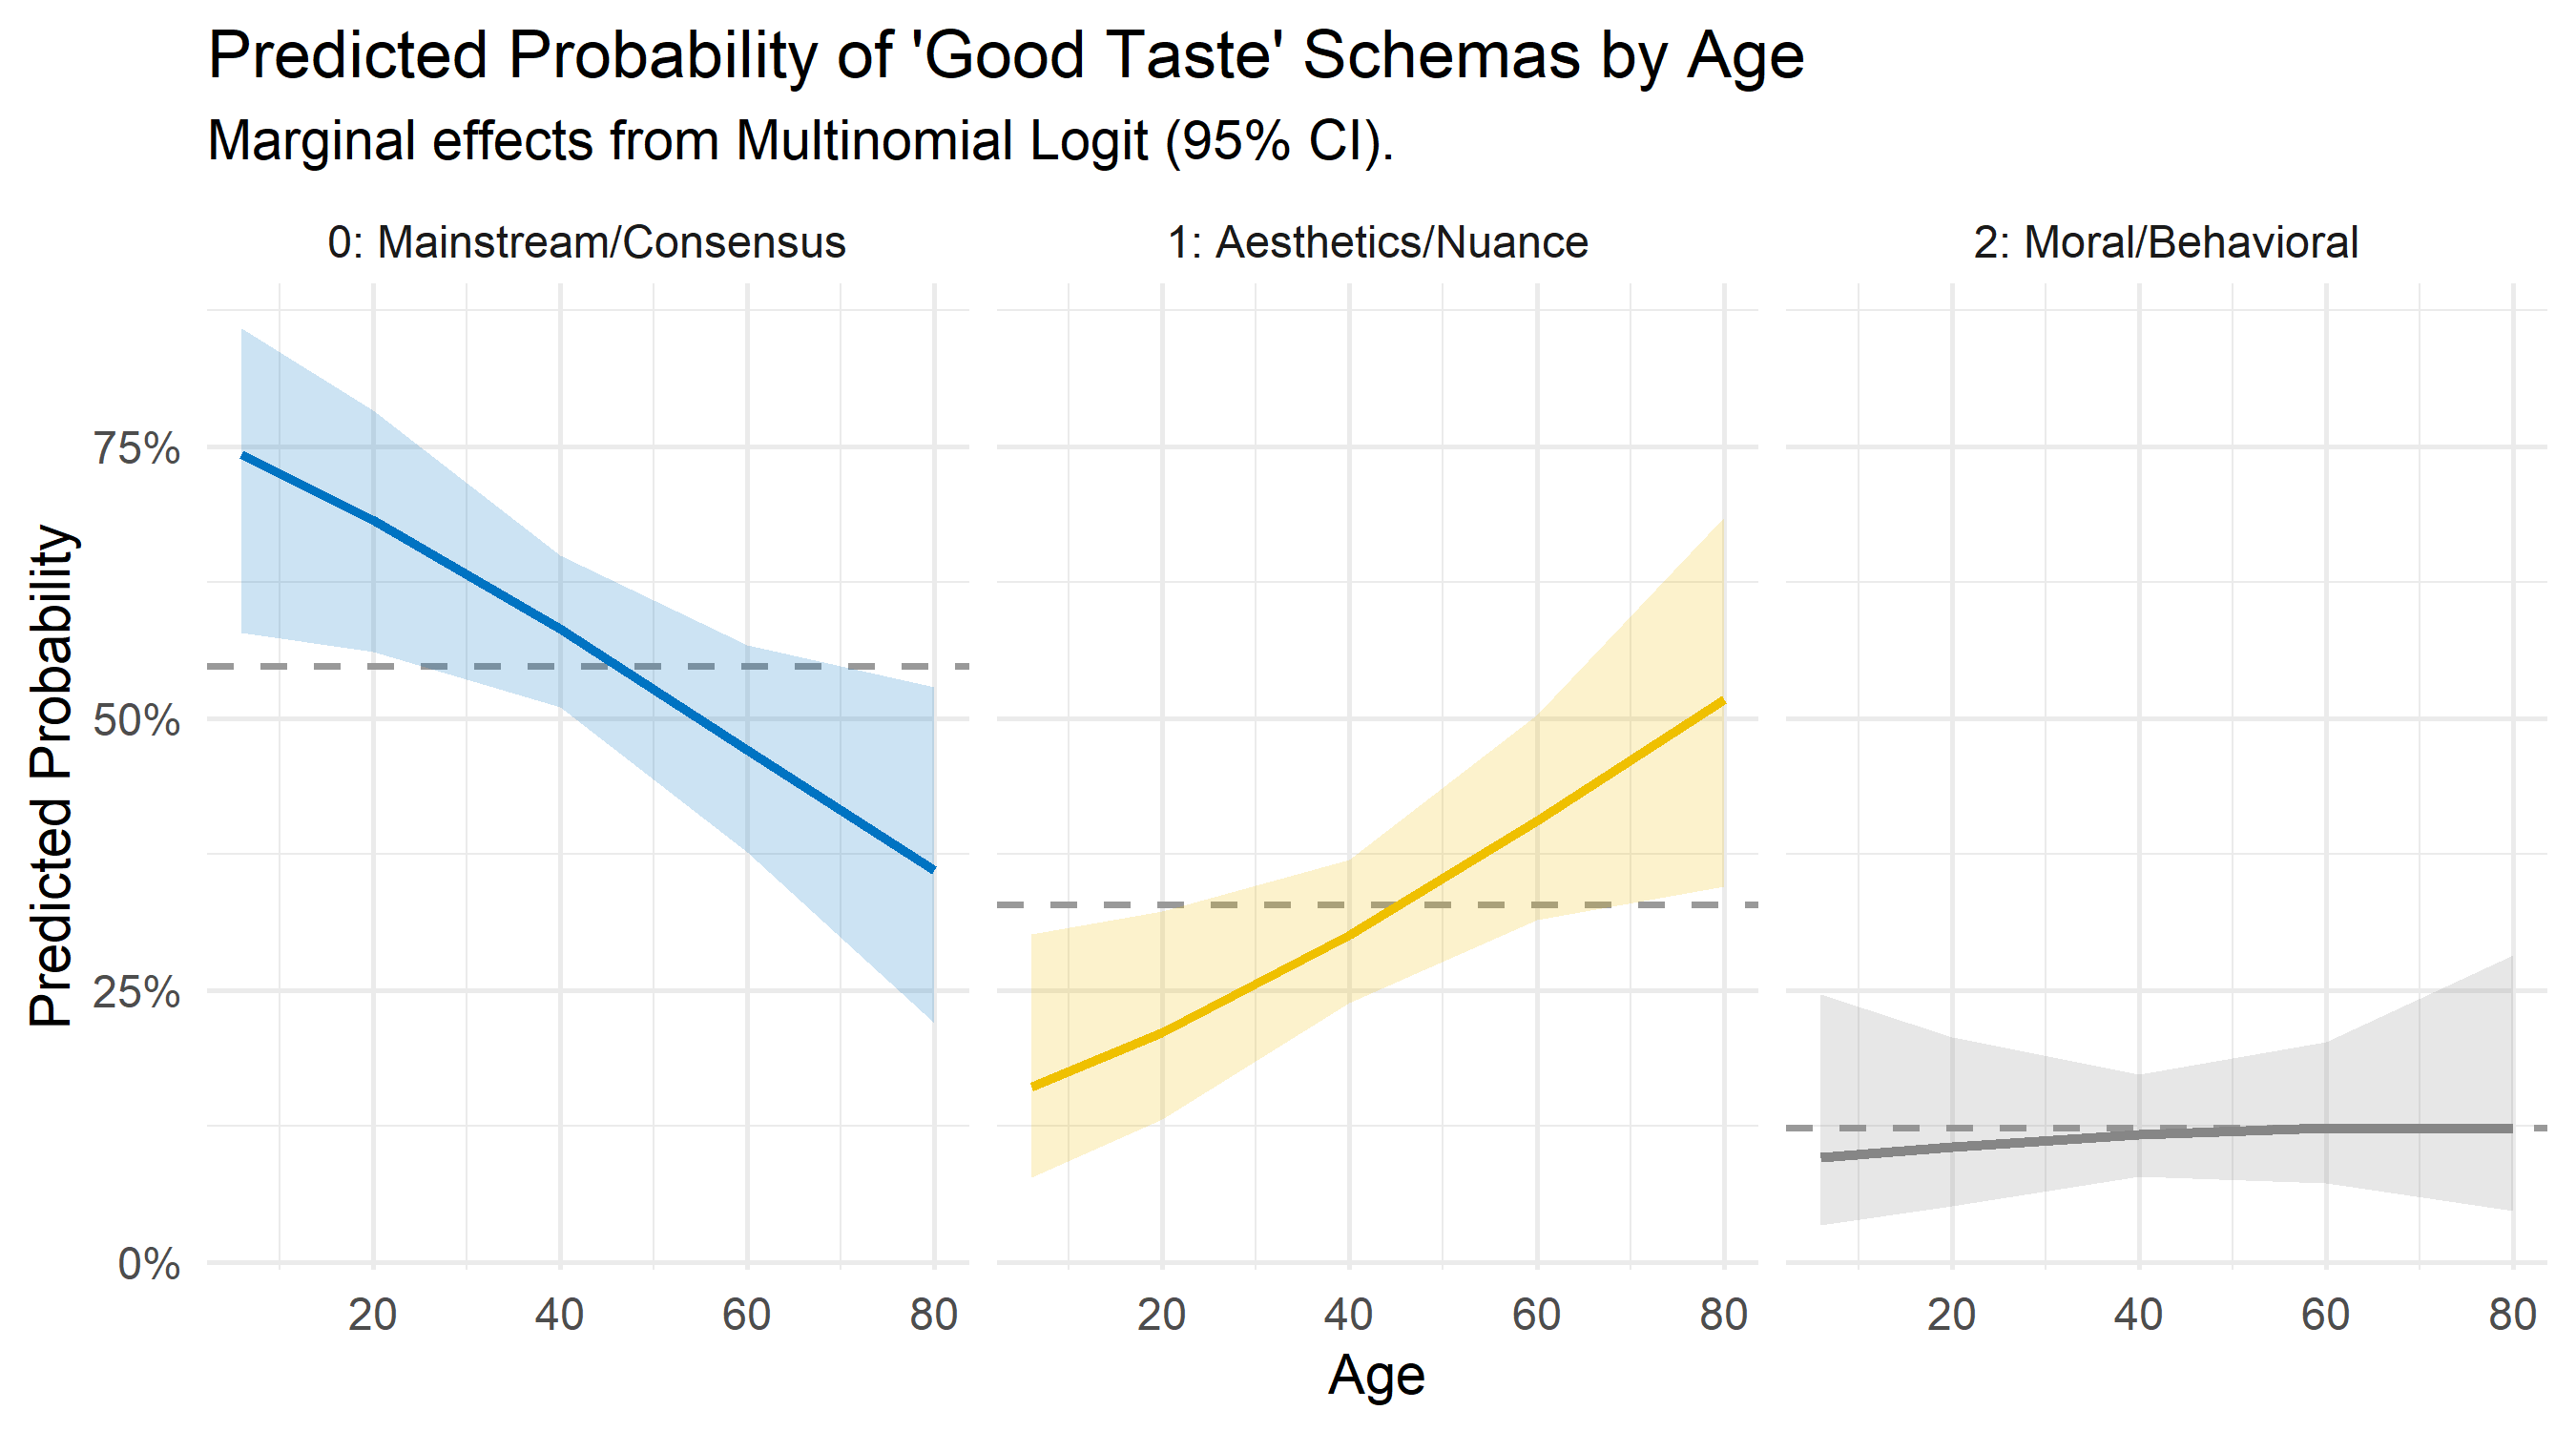
\includegraphics[width=0.48\textwidth]{report/Plots/demographics_good_taste_age.png}
    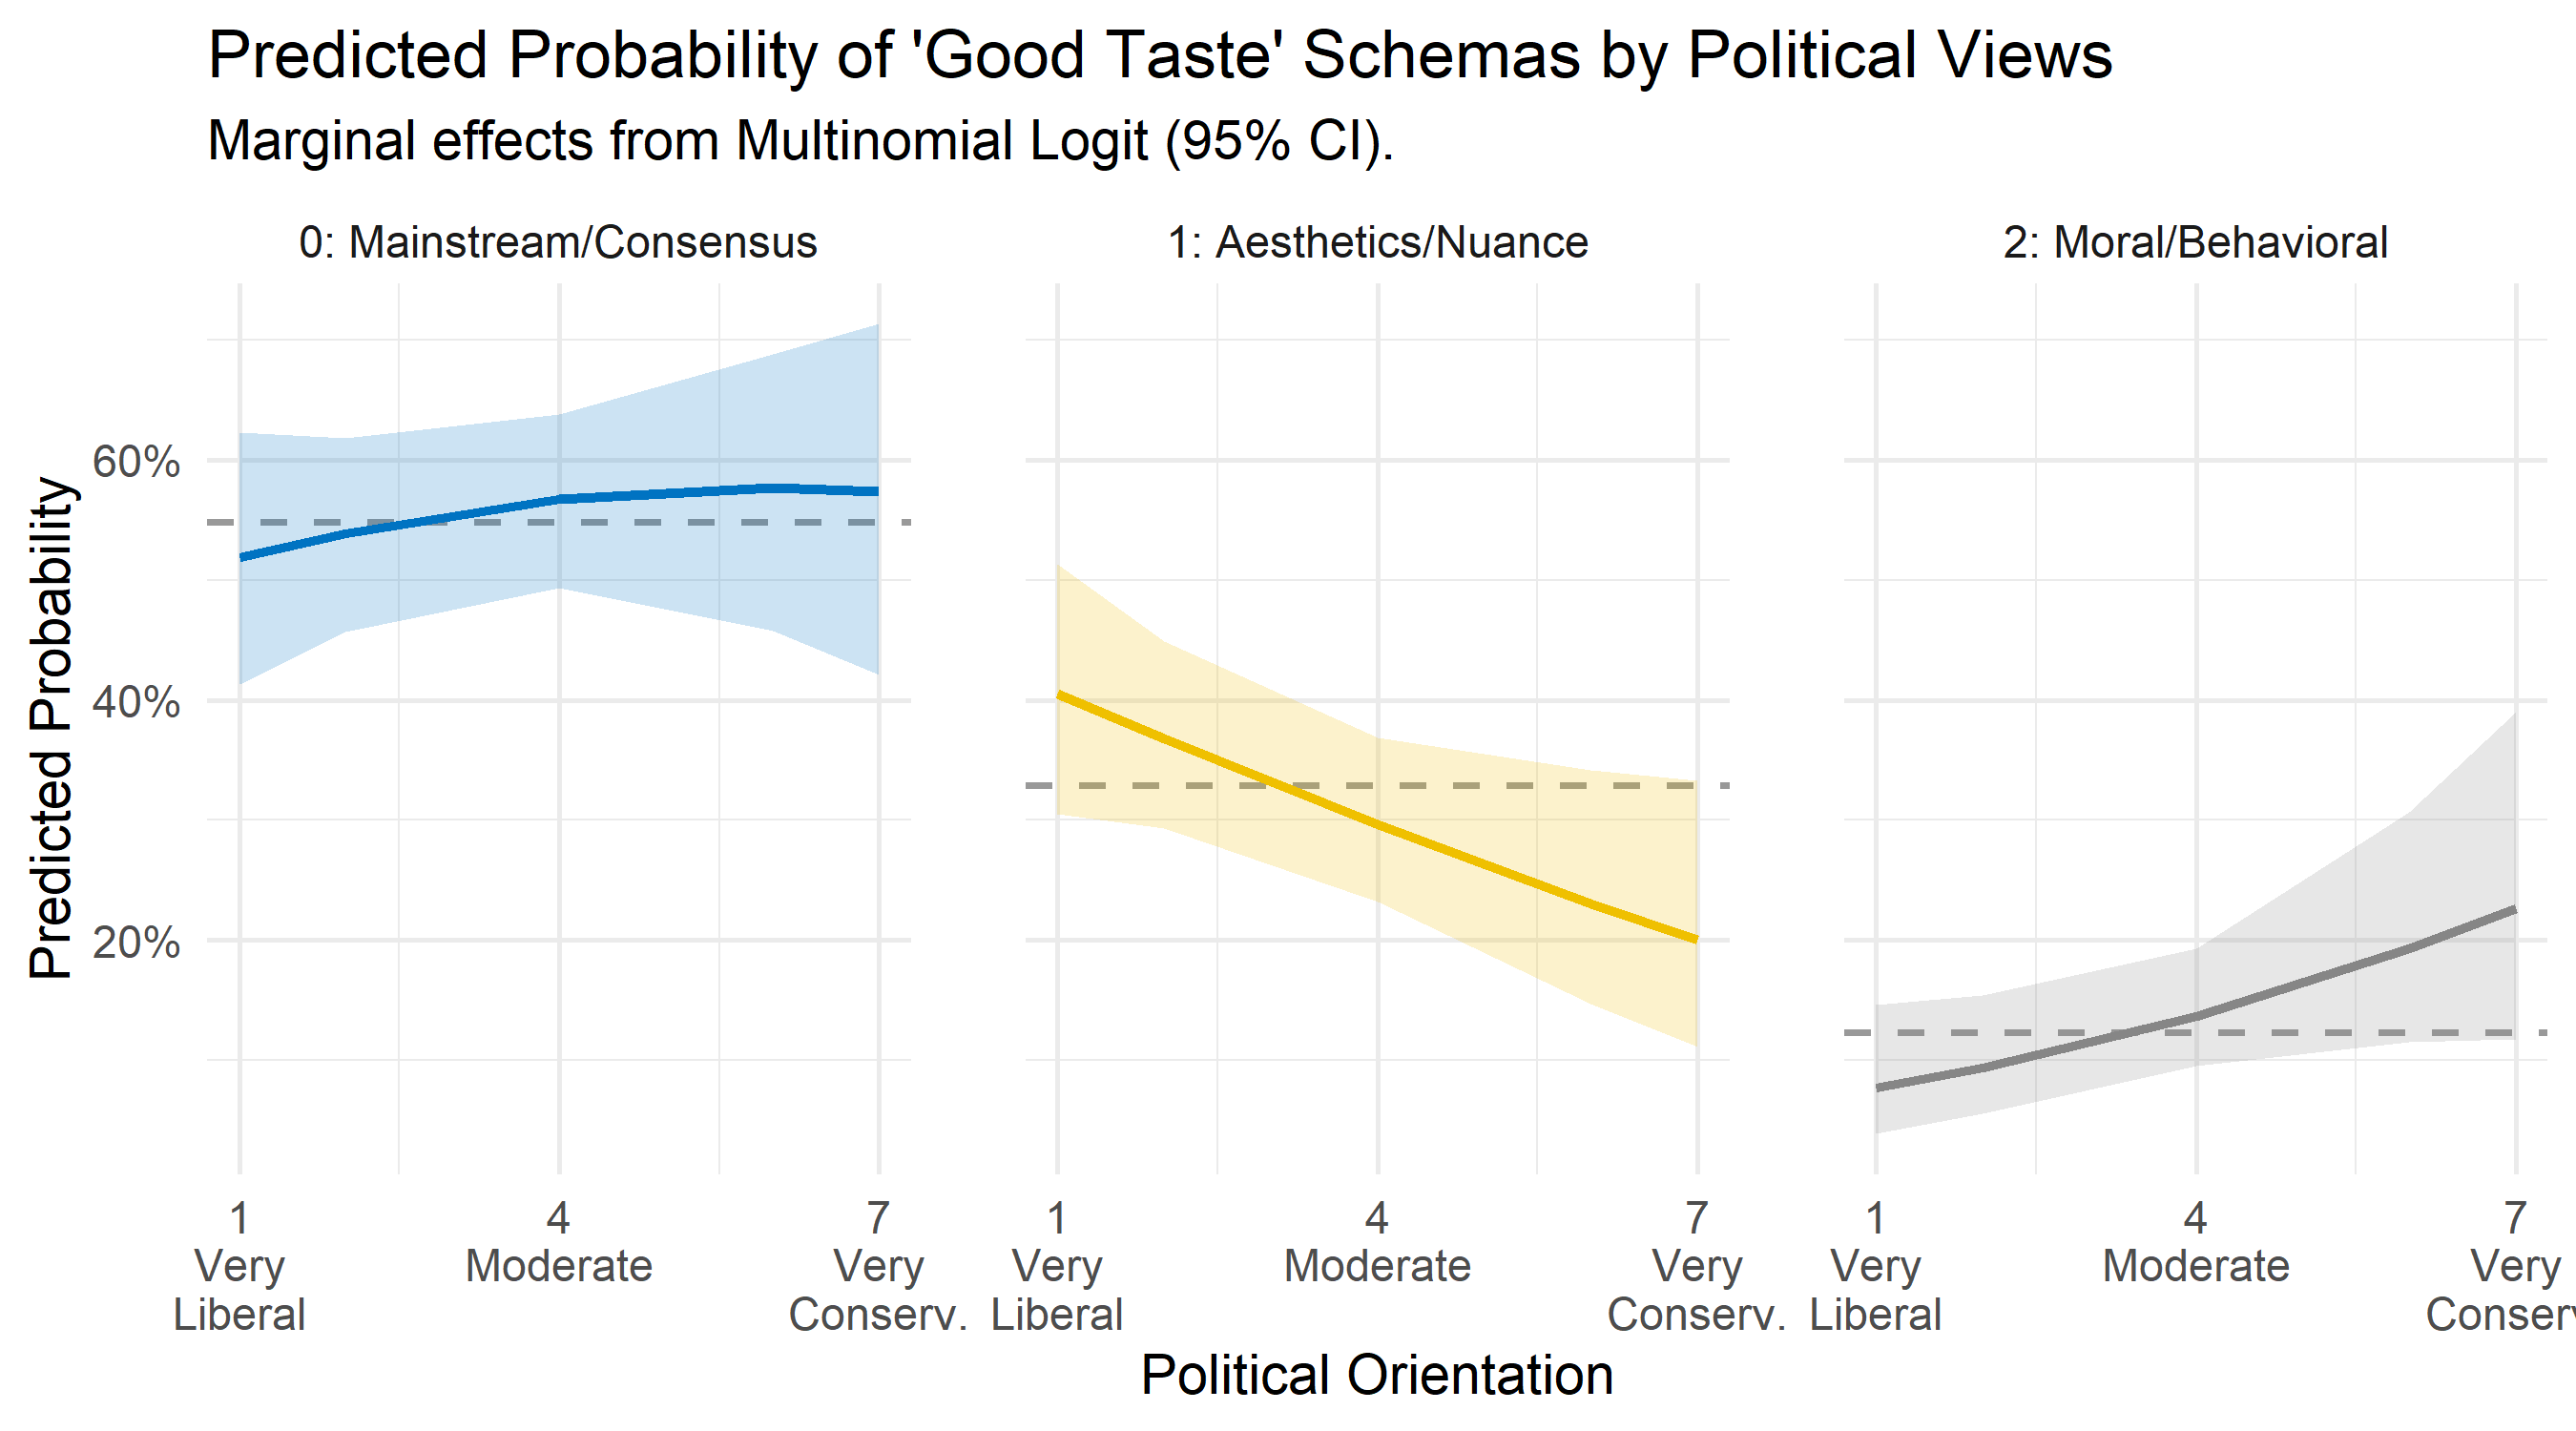
\includegraphics[width=0.48\textwidth]{report/Plots/demographics_good_taste_political.png}
    \caption{Predicted Probability of Good Taste Schemas by Age and Political Views}
    \label{fig:demographics_good}
\end{figure}

\begin{figure}[htpb]
    \centering
    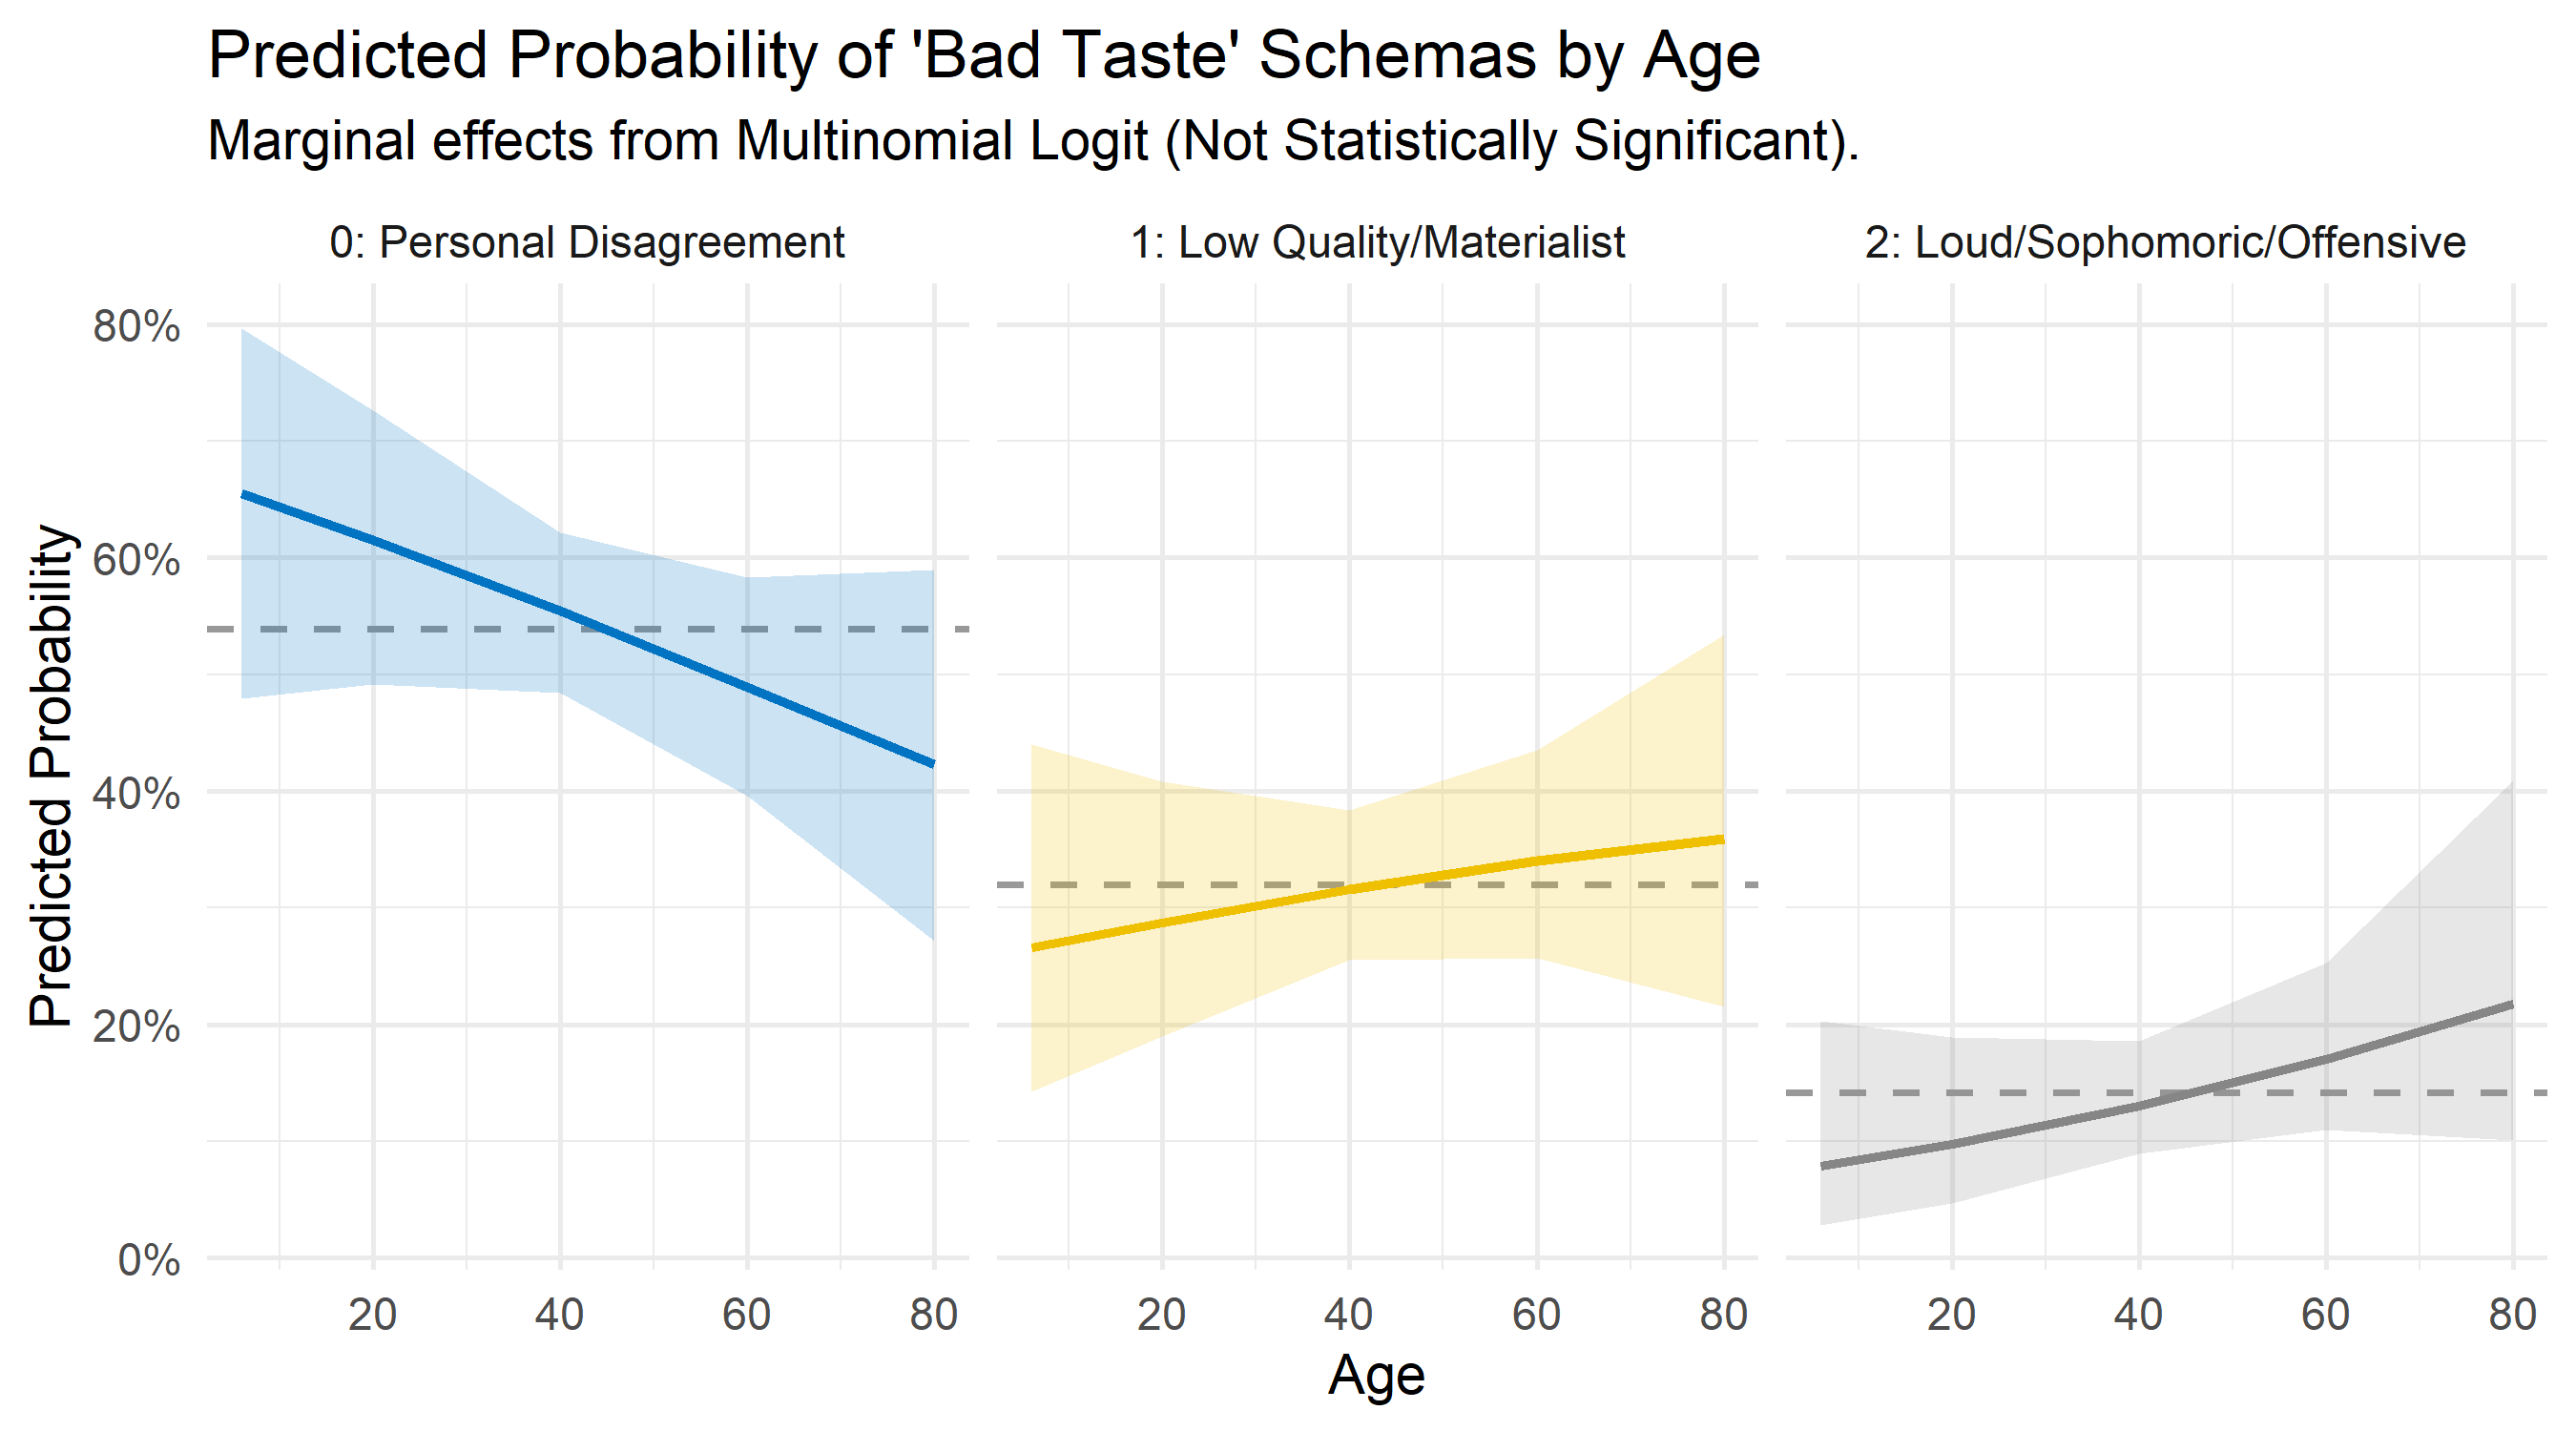
\includegraphics[width=0.5\textwidth]{report/Plots/demographics_bad_taste_age.png}
    \caption{Predicted Probability of Bad Taste Schemas by Age}
    \label{fig:demographics_bad}
\end{figure}

\subsection{Domain Distinction Heatmaps}

Respondents were also asked to rate whether it ``makes sense'' to distinguish good and bad taste across 19 different domains (from -3 = Strongly Disagree to +3 = Strongly Agree). 

Visualizing these scores as heatmaps across our topic clusters reveals several structural universals: regardless of the schema, respondents highly agree that taste distinctions make sense for \textbf{Clothing, Interior Design, Movies, Music, and Paintings}, while rejecting taste distinctions for \textbf{Car Races and Wrestling}.

\begin{figure}[htpb]
    \centering
    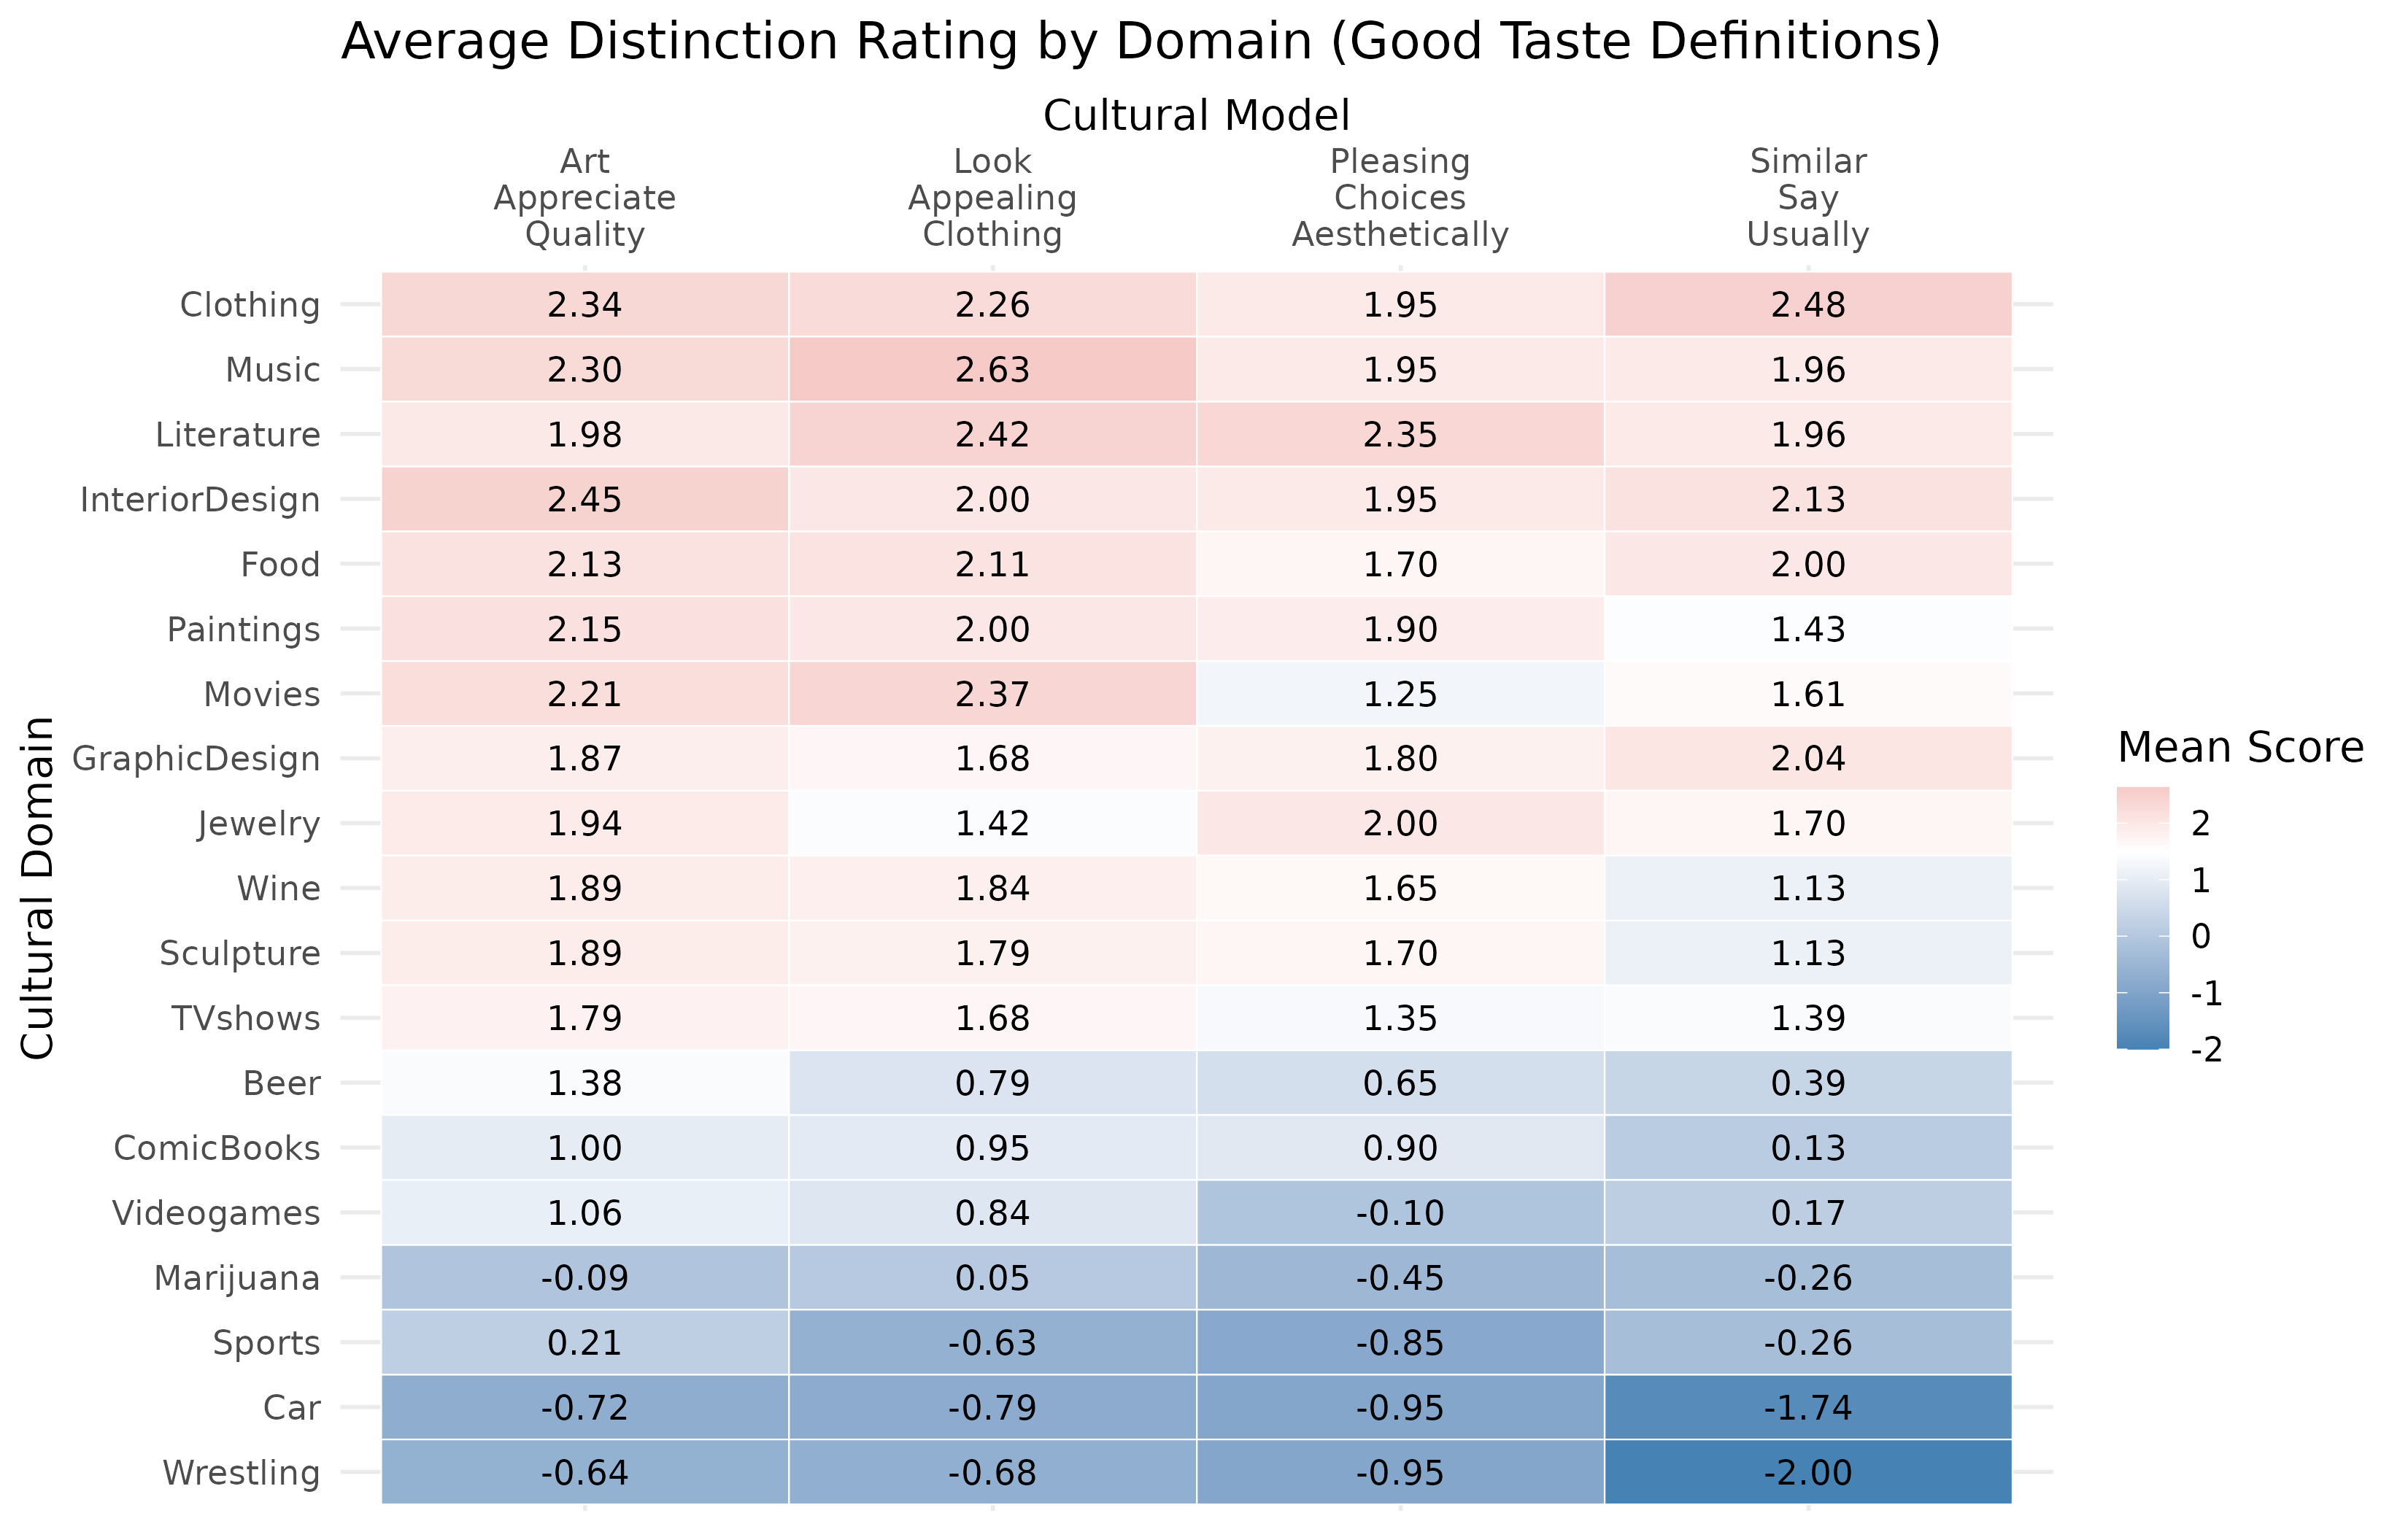
\includegraphics[width=0.8\textwidth]{report/Plots/distinction_domains.png}
    \caption{Average Distinction Rating by Domain and Good Taste Schema}
    \label{fig:distinction_good}
\end{figure}

\begin{figure}[htpb]
    \centering
    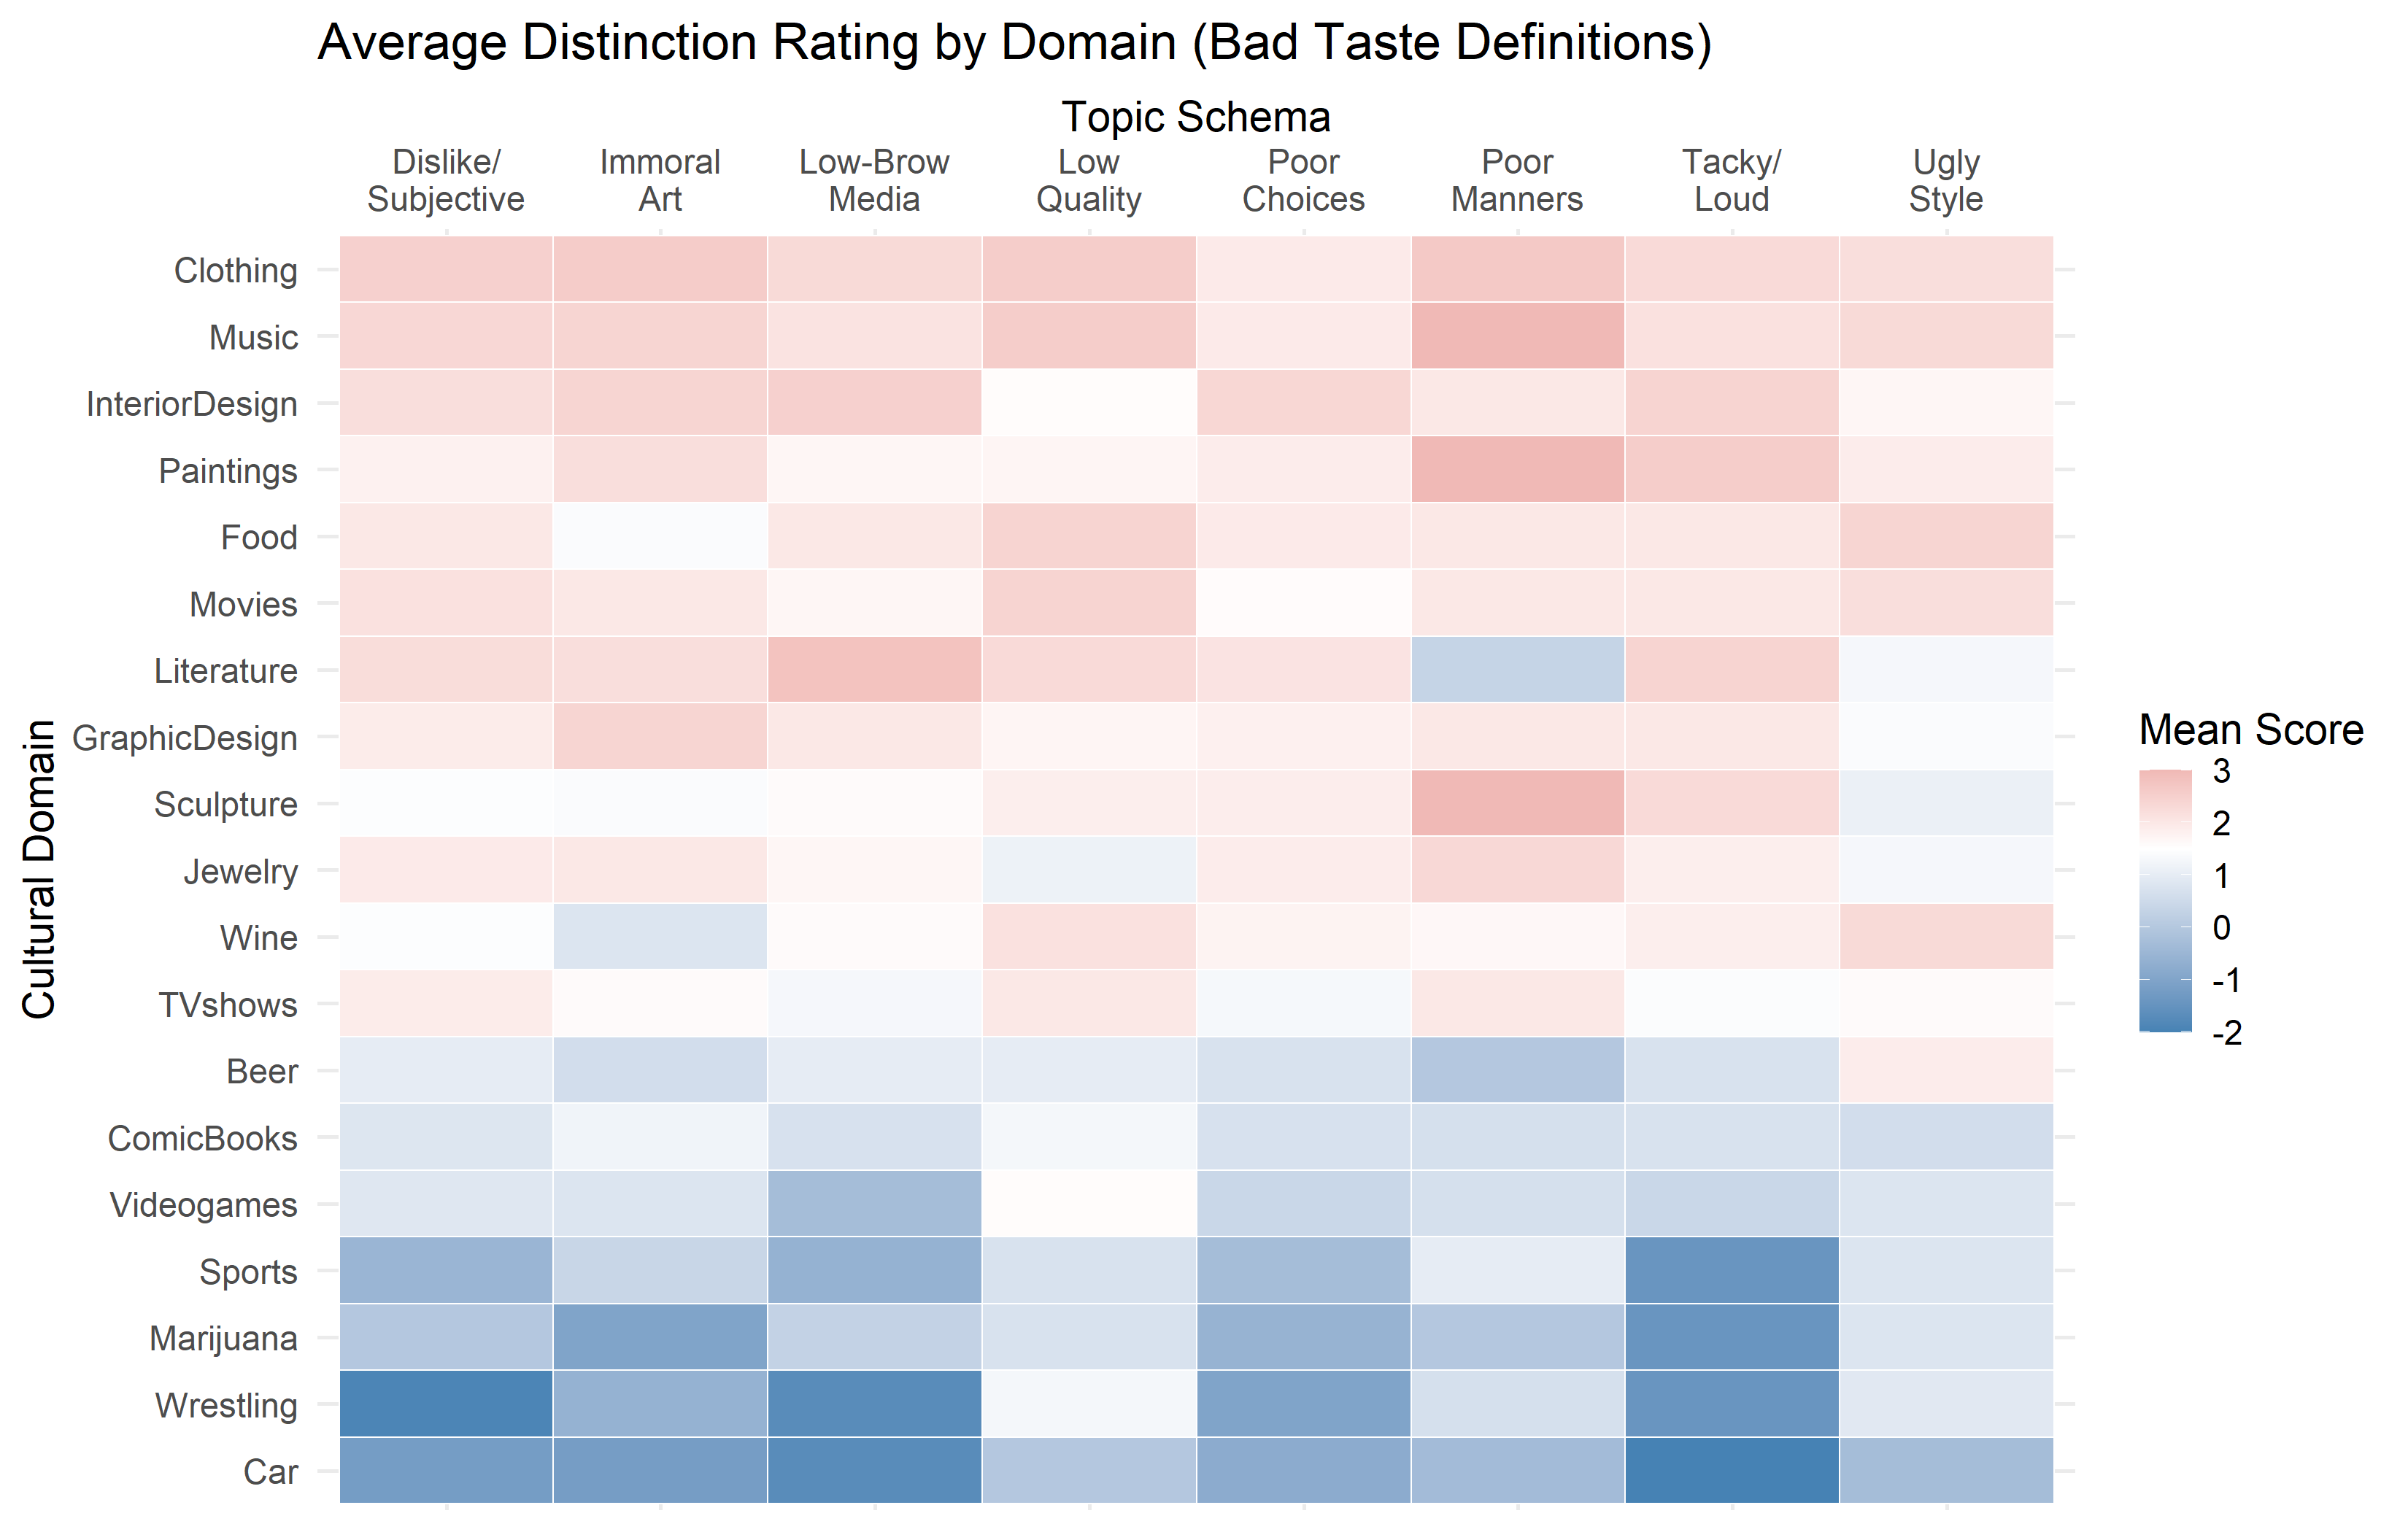
\includegraphics[width=0.8\textwidth]{report/Plots/distinction_domains_bad.png}
    \caption{Average Distinction Rating by Domain and Bad Taste Schema}
    \label{fig:distinction_bad}
\end{figure}

However, there is critical variance in boundary intensity. Respondents whose examples of good taste clustered around \emph{The Obamas/Class}, and whose bad taste clustered around \emph{Trump/Vulgarity}, reported much higher propensity to draw taste distinctions across almost \emph{all} domains, including peripheral ones like Food and Literature. This suggests that when folk models of taste become moralized or politicized, the boundaries of cultural distinction harden and expand across everyday life.

\section{Discussion}

This text-analytic exploration demonstrates that lay definitions of taste are not monolithic; they are multi-dimensional, spanning aesthetic, homophilous, and moral dimensions. Crucially, these dimensions are symmetrical. If an individual views good taste through the lens of objective aesthetic criteria, they evaluate bad taste using the exact same yardstick. 

Furthermore, by mapping these inductively derived cultural models back onto structured survey variables, we observe that the specific folk model an individual uses dictates the breadth of their cultural boundary-drawing. Future research should expand on these findings by examining how these deeply held, qualitative cultural models of taste interact with actual patterns of structural inequality.

\newpage
\bibliographystyle{apalike}
\bibliography{references}

\end{document}